\clearpage

\section{Topic 00}

\begin{figure}[htbp!]
    \centering
    \begin{subfigure}[b]{0.49\textwidth}
        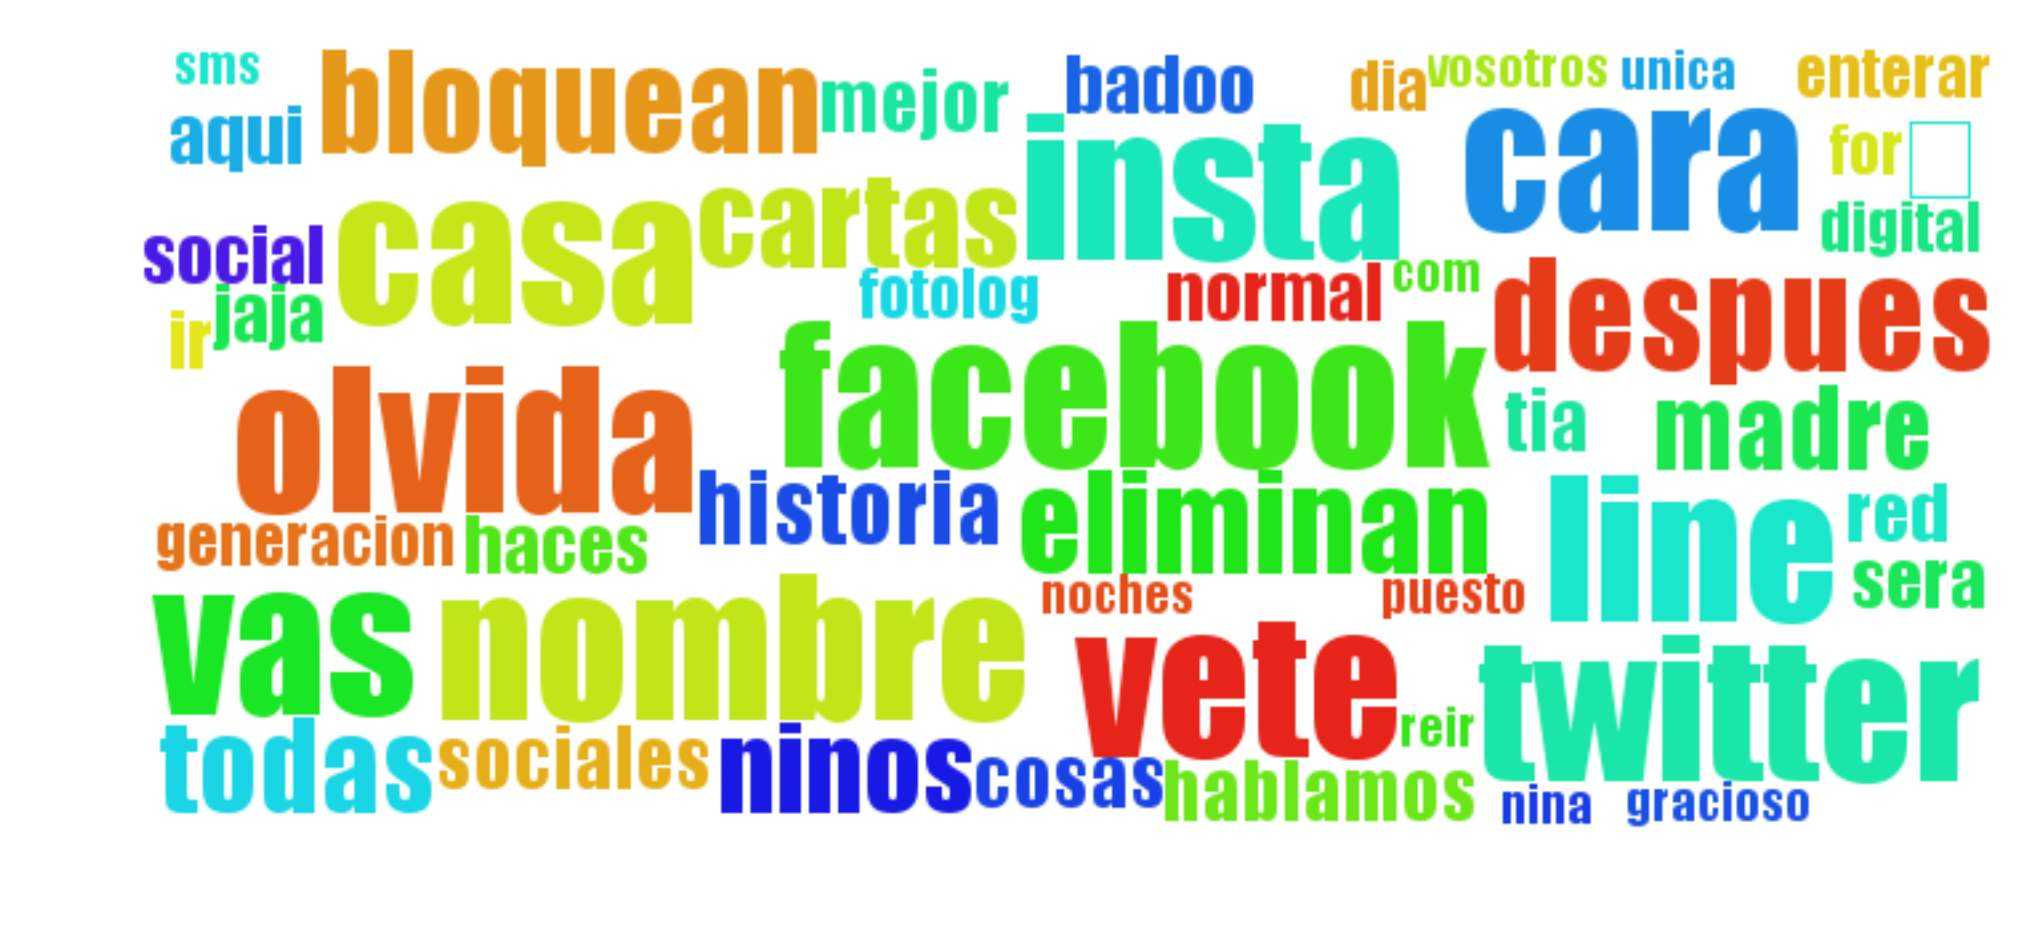
\includegraphics[width=\textwidth]{twitter_murcia/report_images/topic-00-wordcloud.jpg}
    \end{subfigure}
    \begin{subfigure}[b]{0.49\textwidth}
        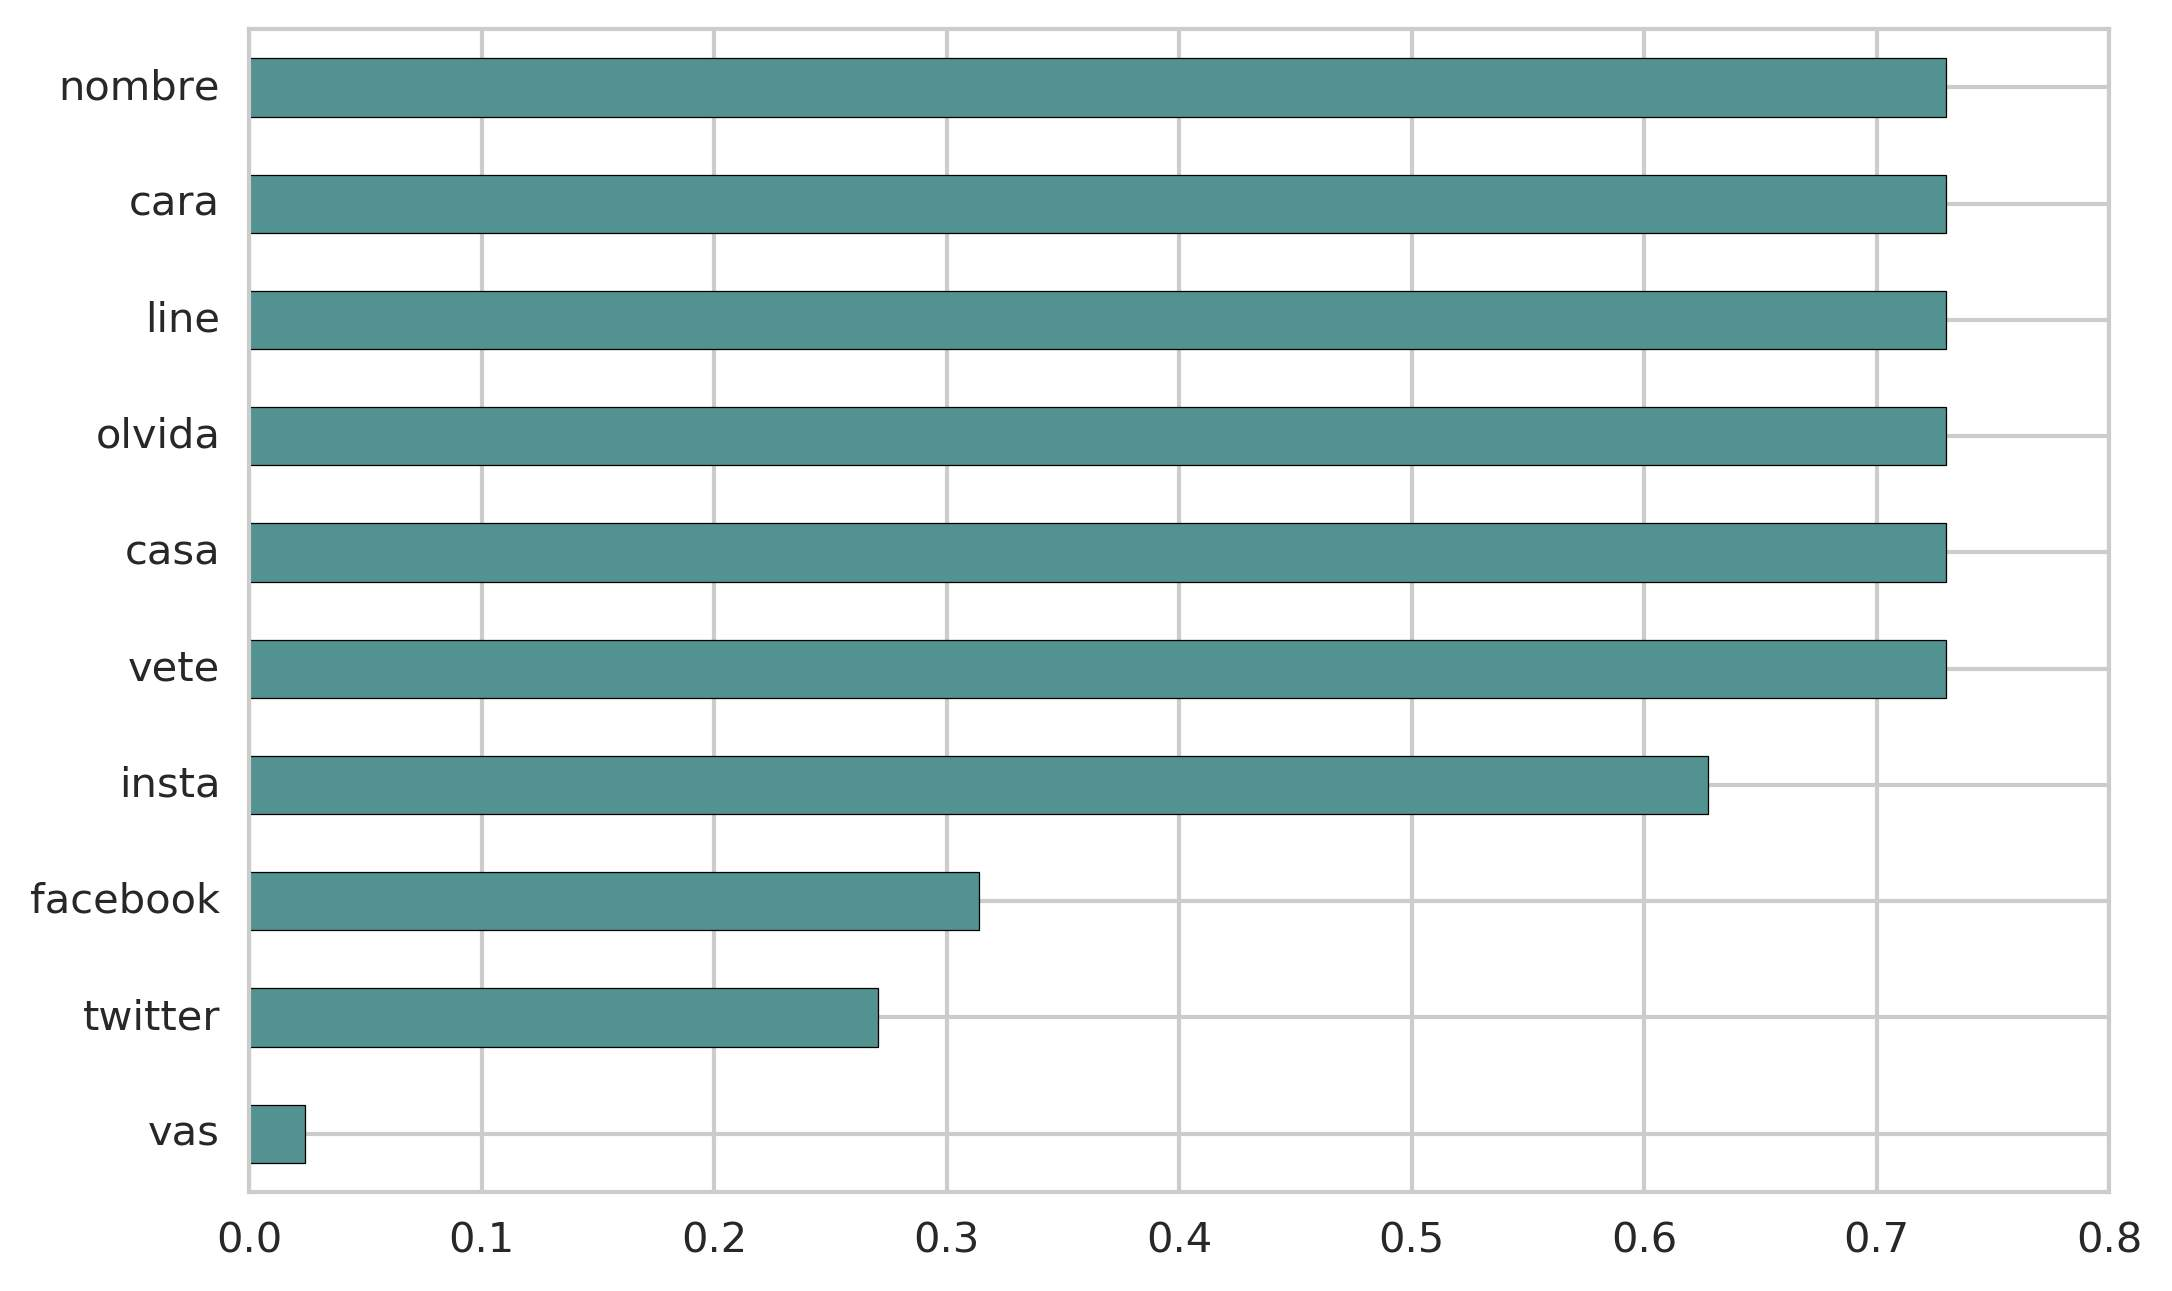
\includegraphics[width=\textwidth]{twitter_murcia/report_images/topic-00-terms.jpg}
    \end{subfigure}
\end{figure}

\begin{figure}[htbp!]
    \centering
    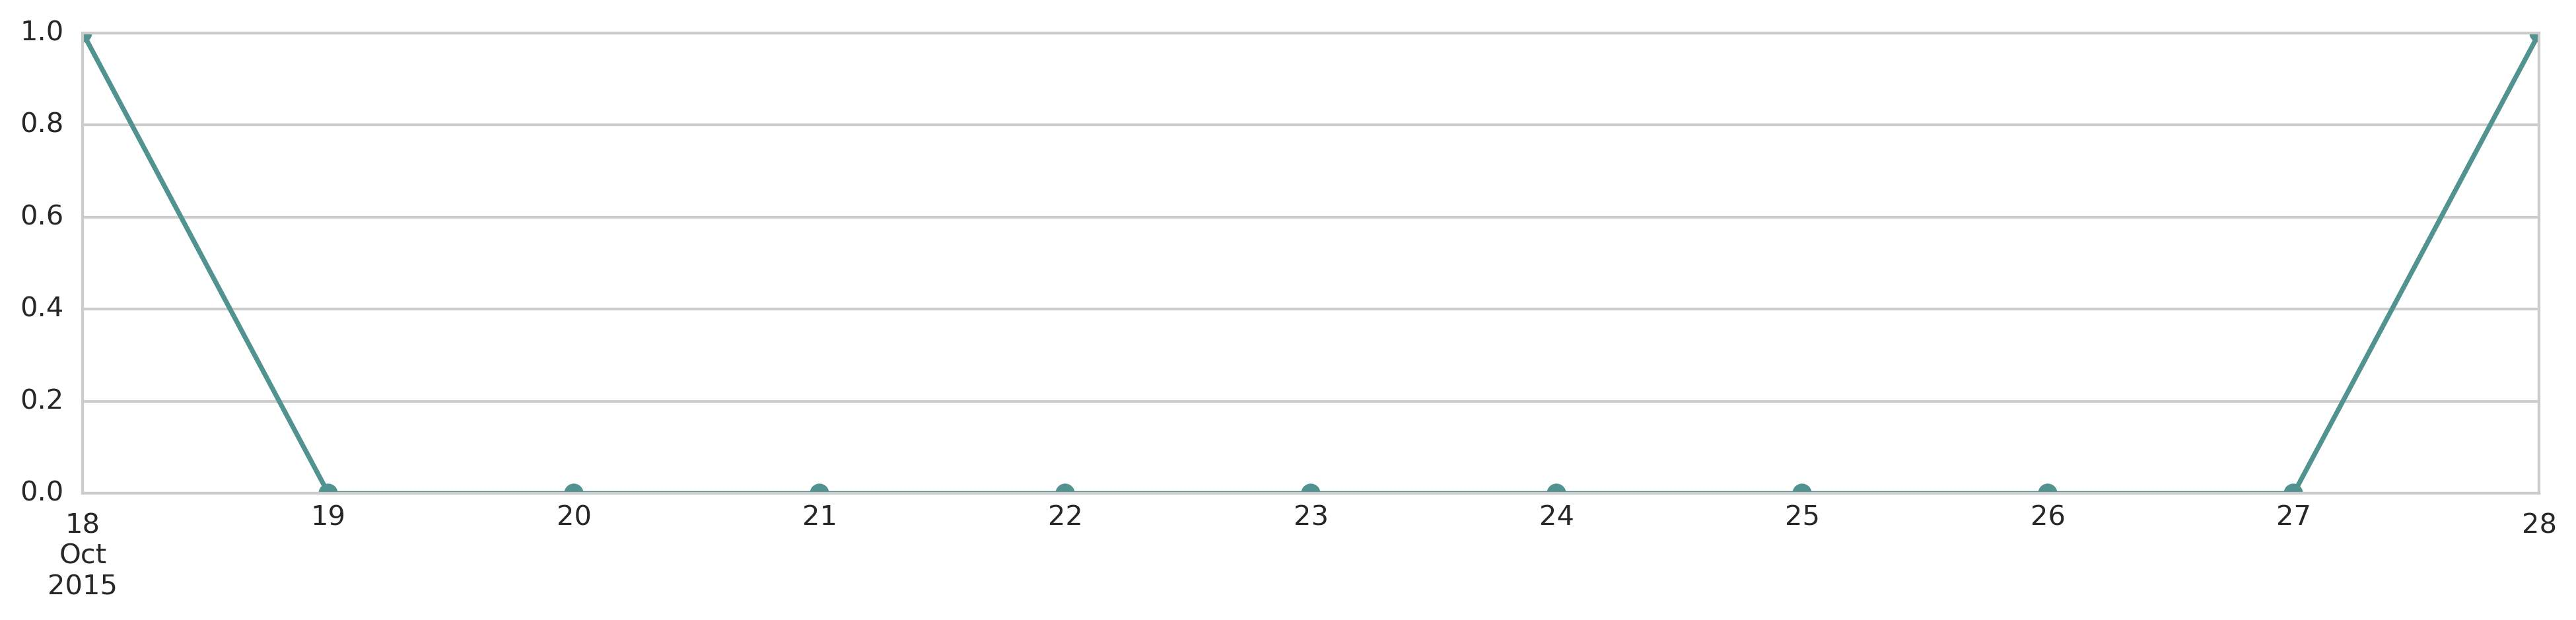
\includegraphics[width=\textwidth]{twitter_murcia/report_images/topic-00-timeseries.jpg}
\end{figure}

\rowcolors{2}{gray!25}{white}
\begin{longtable}{p{12.5cm}rr}
\toprule
Text & Count & Rel \\
\midrule
\endhead
\midrule
\multicolumn{3}{r}{{Continued on next page}} \\
\midrule
\endfoot

\bottomrule
\endlastfoot
\begin{tabular}[c]{@{}l@{}}RT @baterianakama: Por eso, vete, olvida mi nombre, mi cara, mi casa: \\ Mi Twitter \\ Mi Facebook \\ Mi Tuenti \\ Mi Insta. \\ Mi Wassap \\ Mi Line \\ Mi Tumbl…\end{tabular} & 2 & 1.00 \\

\end{longtable}
\clearpage

\section{Topic 01}

\begin{figure}[htbp!]
    \centering
    \begin{subfigure}[b]{0.49\textwidth}
        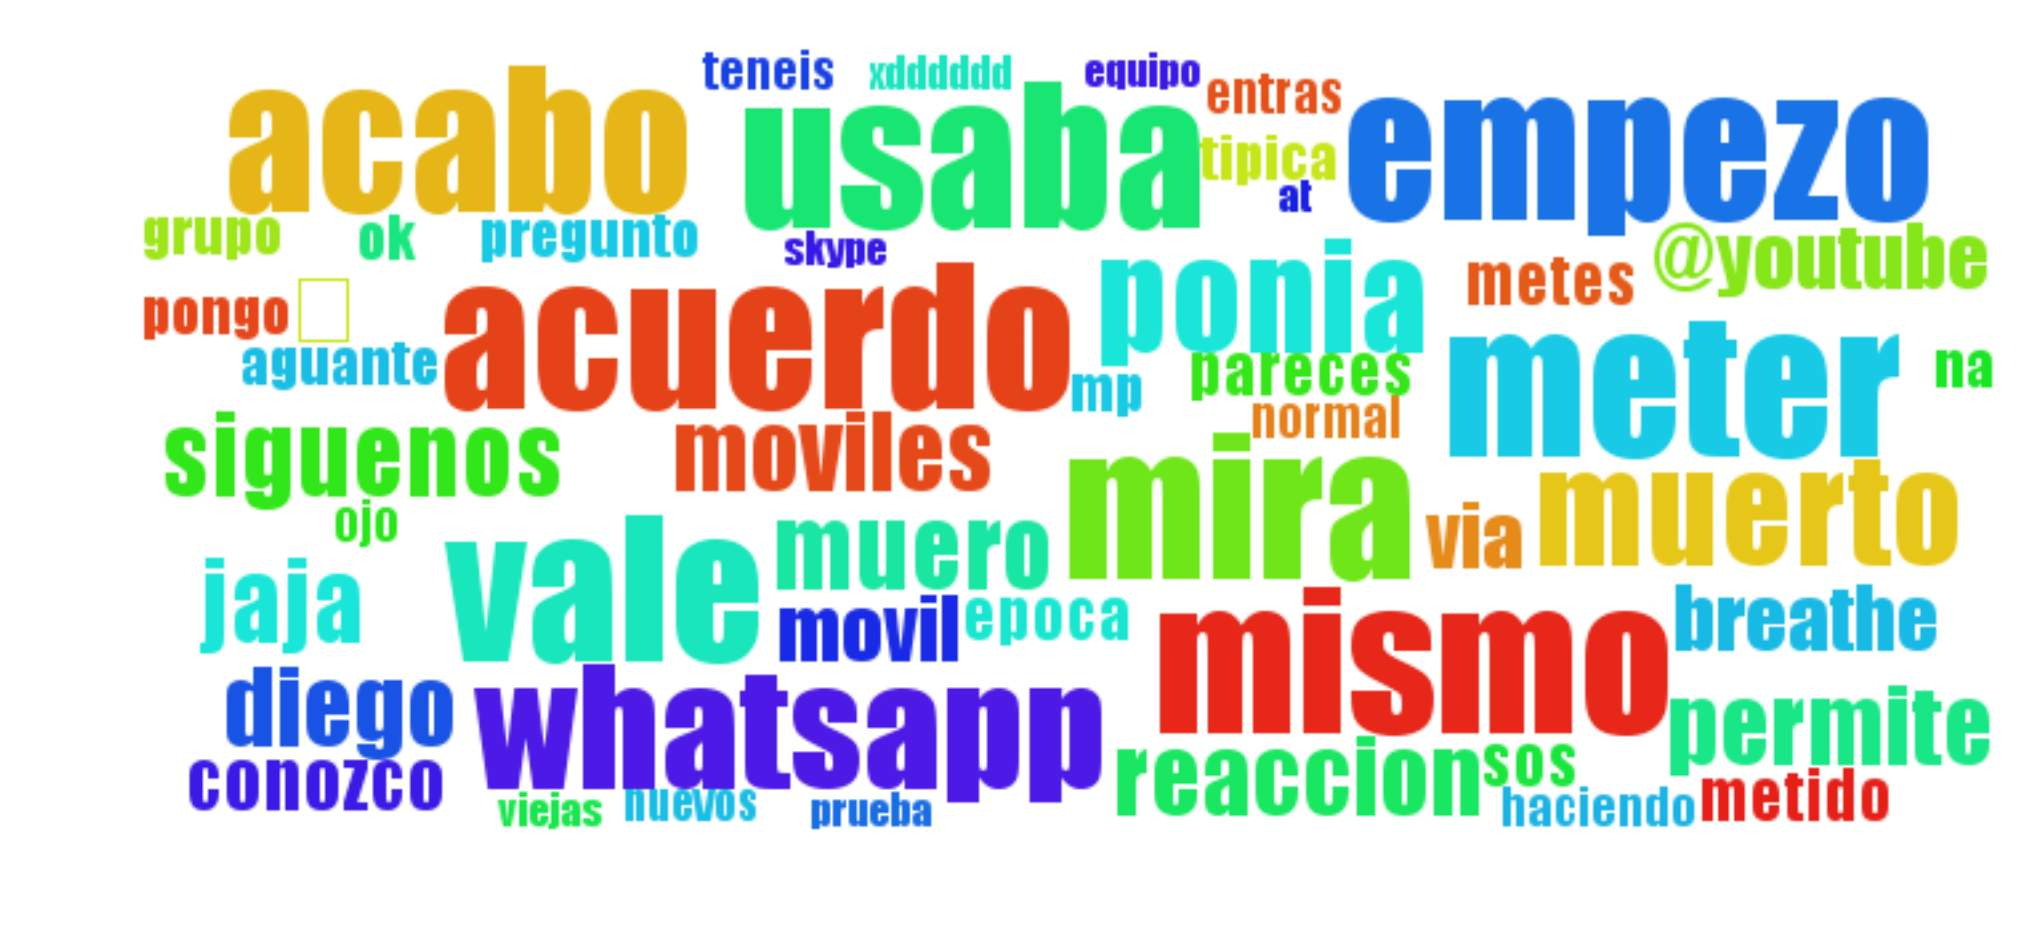
\includegraphics[width=\textwidth]{twitter_murcia/report_images/topic-01-wordcloud.jpg}
    \end{subfigure}
    \begin{subfigure}[b]{0.49\textwidth}
        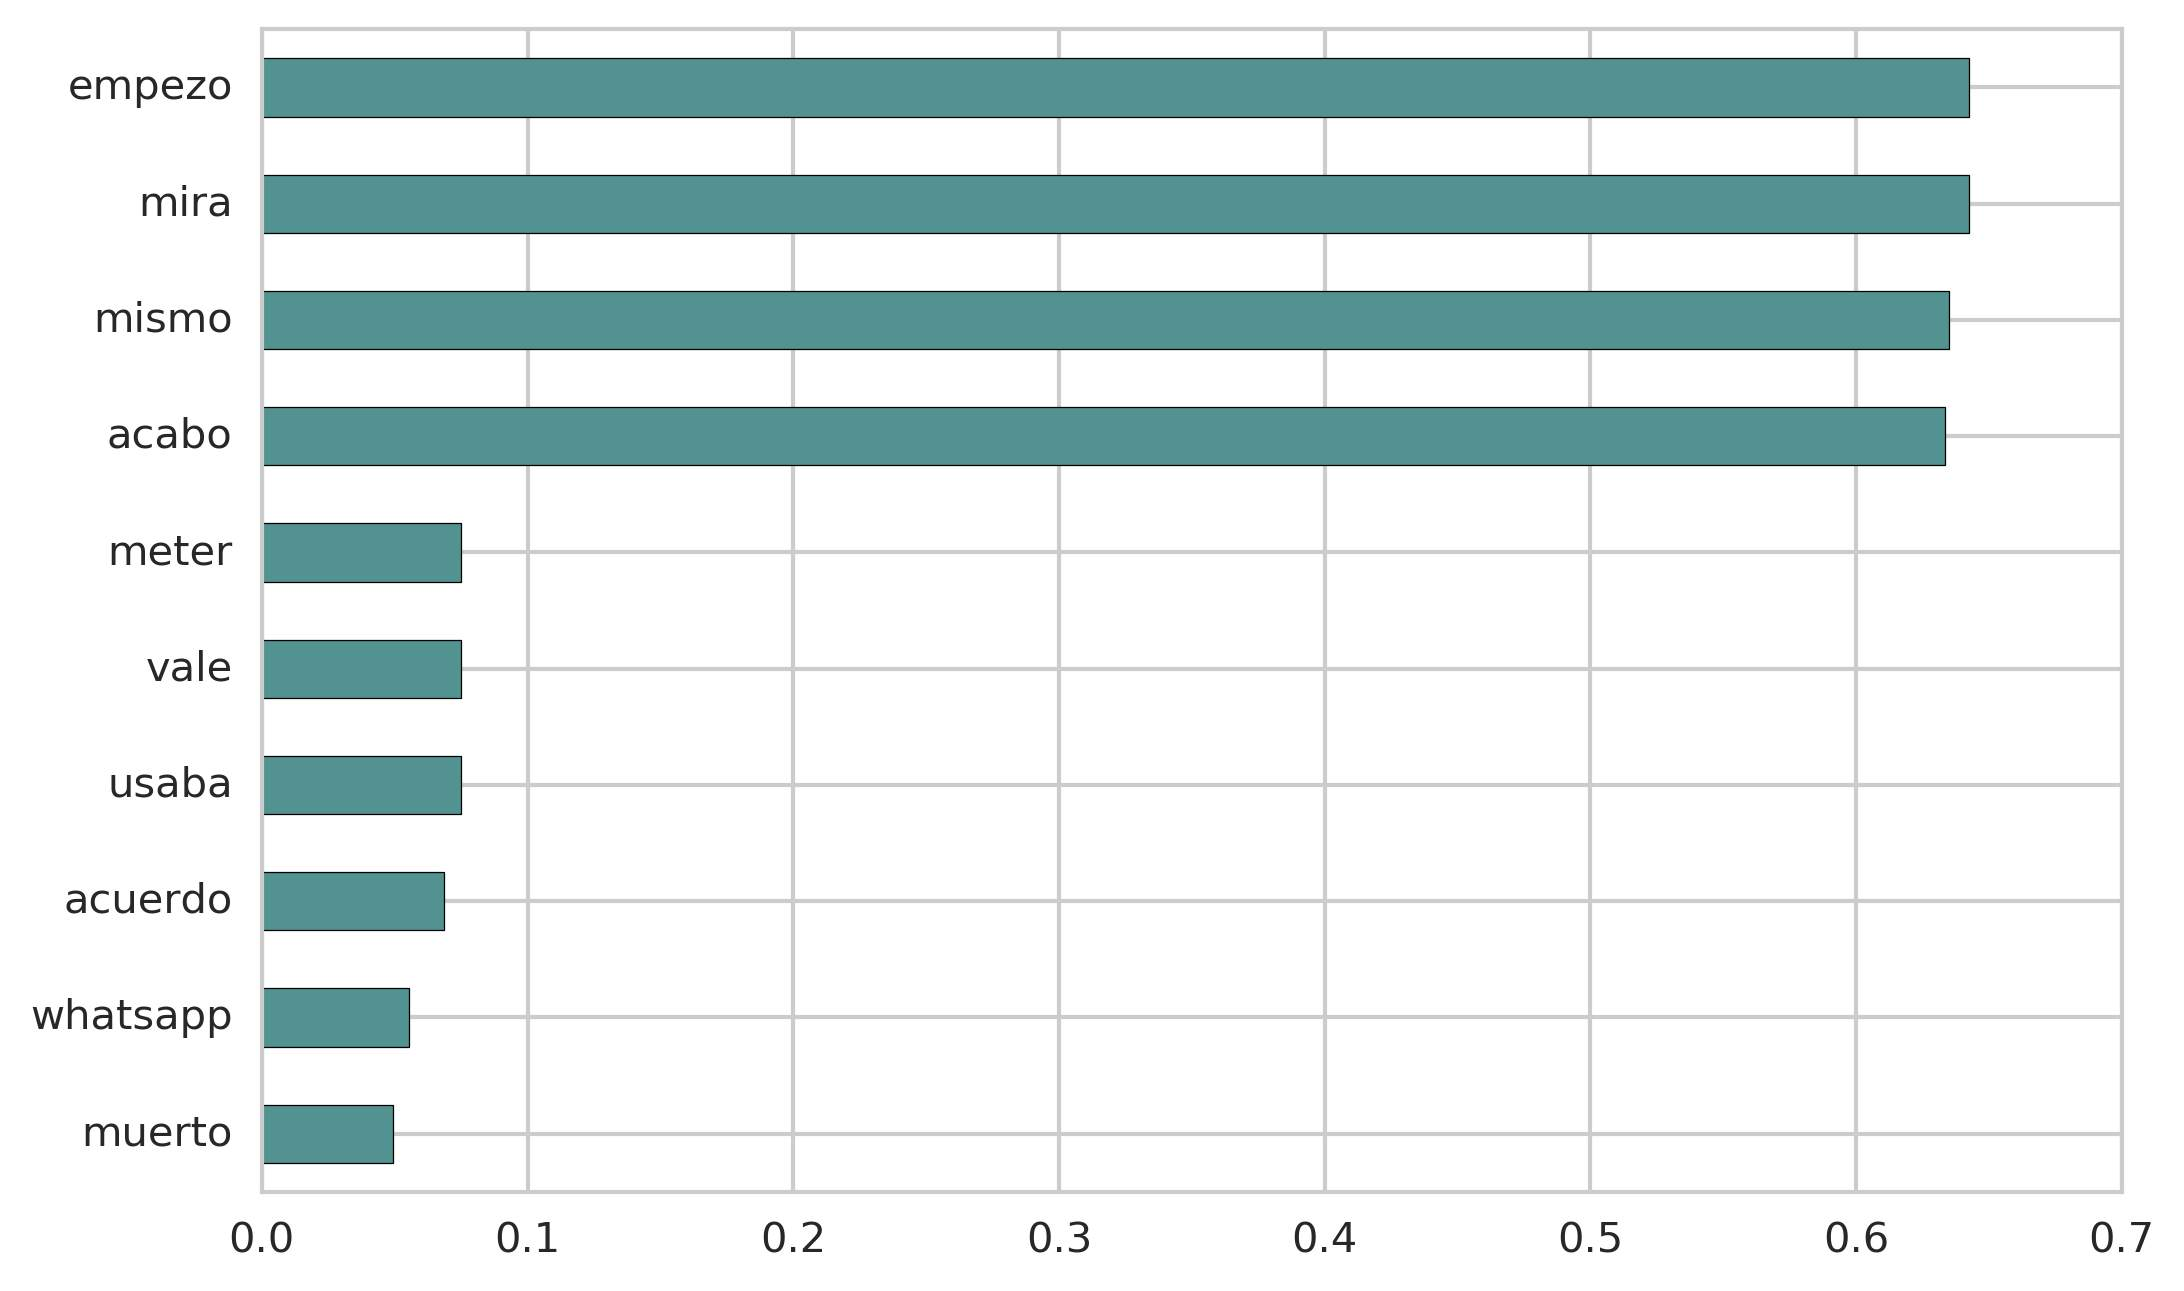
\includegraphics[width=\textwidth]{twitter_murcia/report_images/topic-01-terms.jpg}
    \end{subfigure}
\end{figure}

\begin{figure}[htbp!]
    \centering
    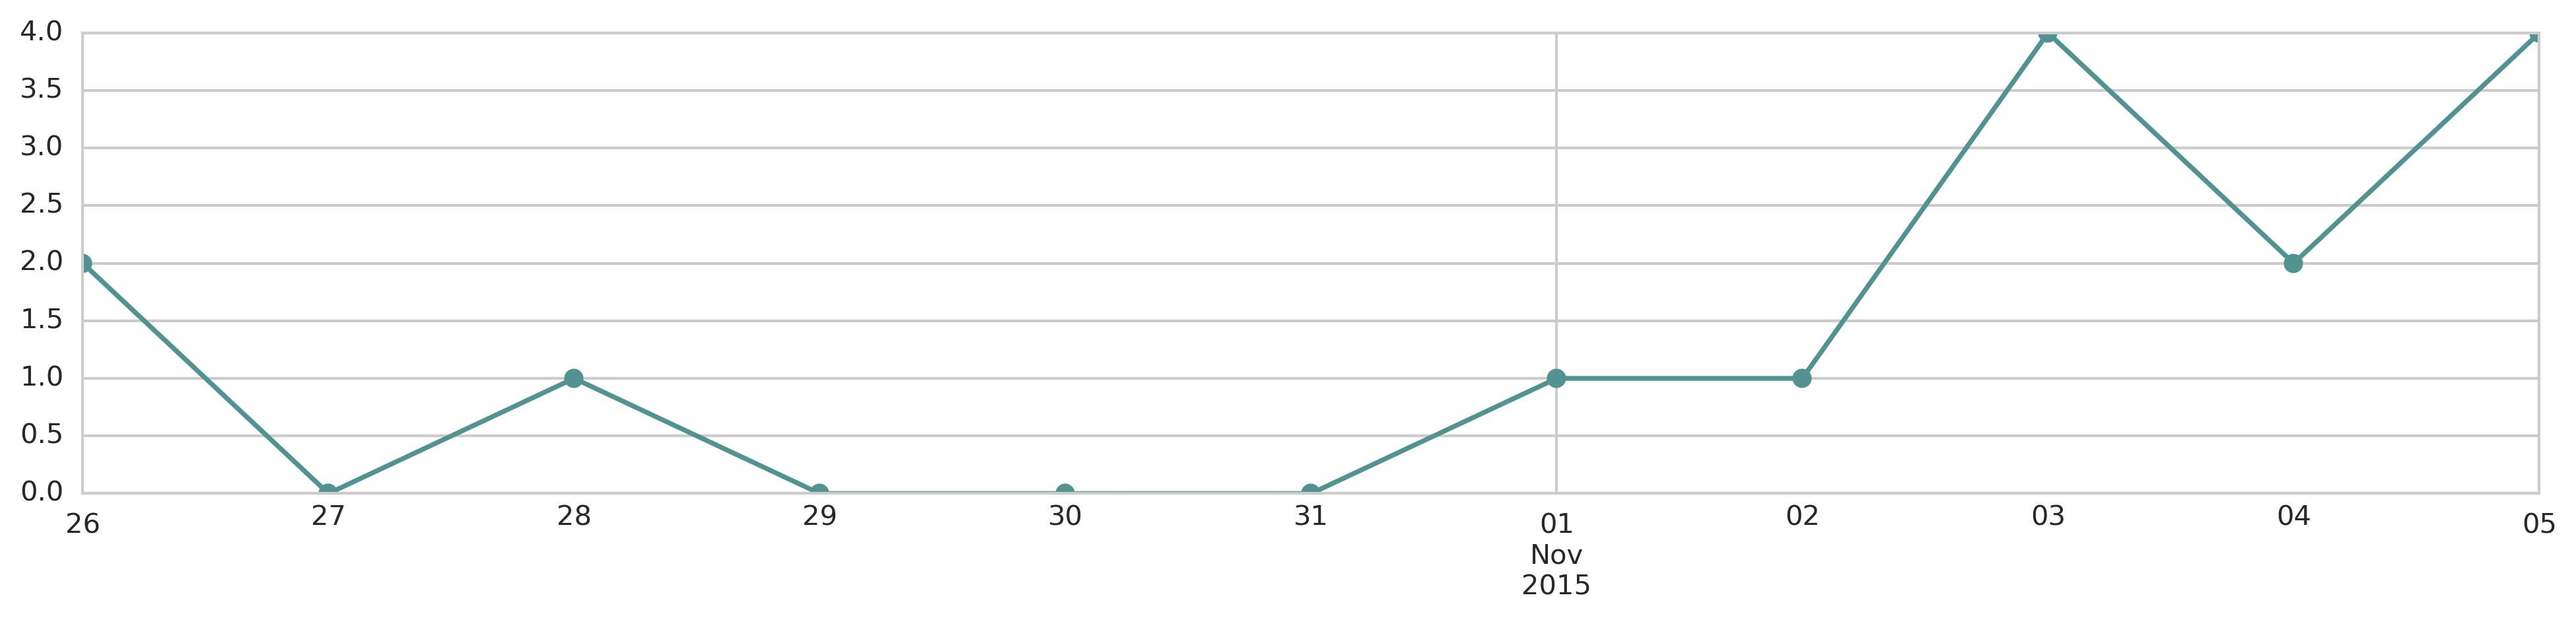
\includegraphics[width=\textwidth]{twitter_murcia/report_images/topic-01-timeseries.jpg}
\end{figure}

\rowcolors{2}{gray!25}{white}
\begin{longtable}{p{12.5cm}rr}
\toprule
Text & Count & Rel \\
\midrule
\endhead
\midrule
\multicolumn{3}{r}{{Continued on next page}} \\
\midrule
\endfoot

\bottomrule
\endlastfoot
RT @VictorEmeceh: Tuenti empezó cambiando un poco, y mira como acabo. @Twitter esperemos que no hayas contratado al mismo diseñador, os lo … & 9 & 0.99 \\
Me acabo de meter a Tuenti vale y no me acuerdo de como se usaba eso 😂😂 & 1 & 0.19 \\
RT @MrsPizzzza: Mi whatsapp ahora mismo está más muerto que el tuenti de todos nosotros & 1 & 0.18 \\
@jaime\_salinas92 Tuenti está muerto & 1 & 0.04 \\
Reacción a mi Tuenti | Diego Breathe https://t.co/zMmkogZ6WA vía @YouTube & 1 & 0.02 \\
RT @DeseoLiterario: Reacción a mi Tuenti | Diego Breathe https://t.co/zMmkogZ6WA vía @YouTube & 1 & 0.02 \\
Pepeenergy de Pepephone y Móvil sin Móvil de .Tuenti, innovaciones 2015 \#PremiosADSLZone https://t.co/TUSrOtMGK1 via @adslzone & 1 & 0.00 \\

\end{longtable}
\clearpage

\section{Topic 02}

\begin{figure}[htbp!]
    \centering
    \begin{subfigure}[b]{0.49\textwidth}
        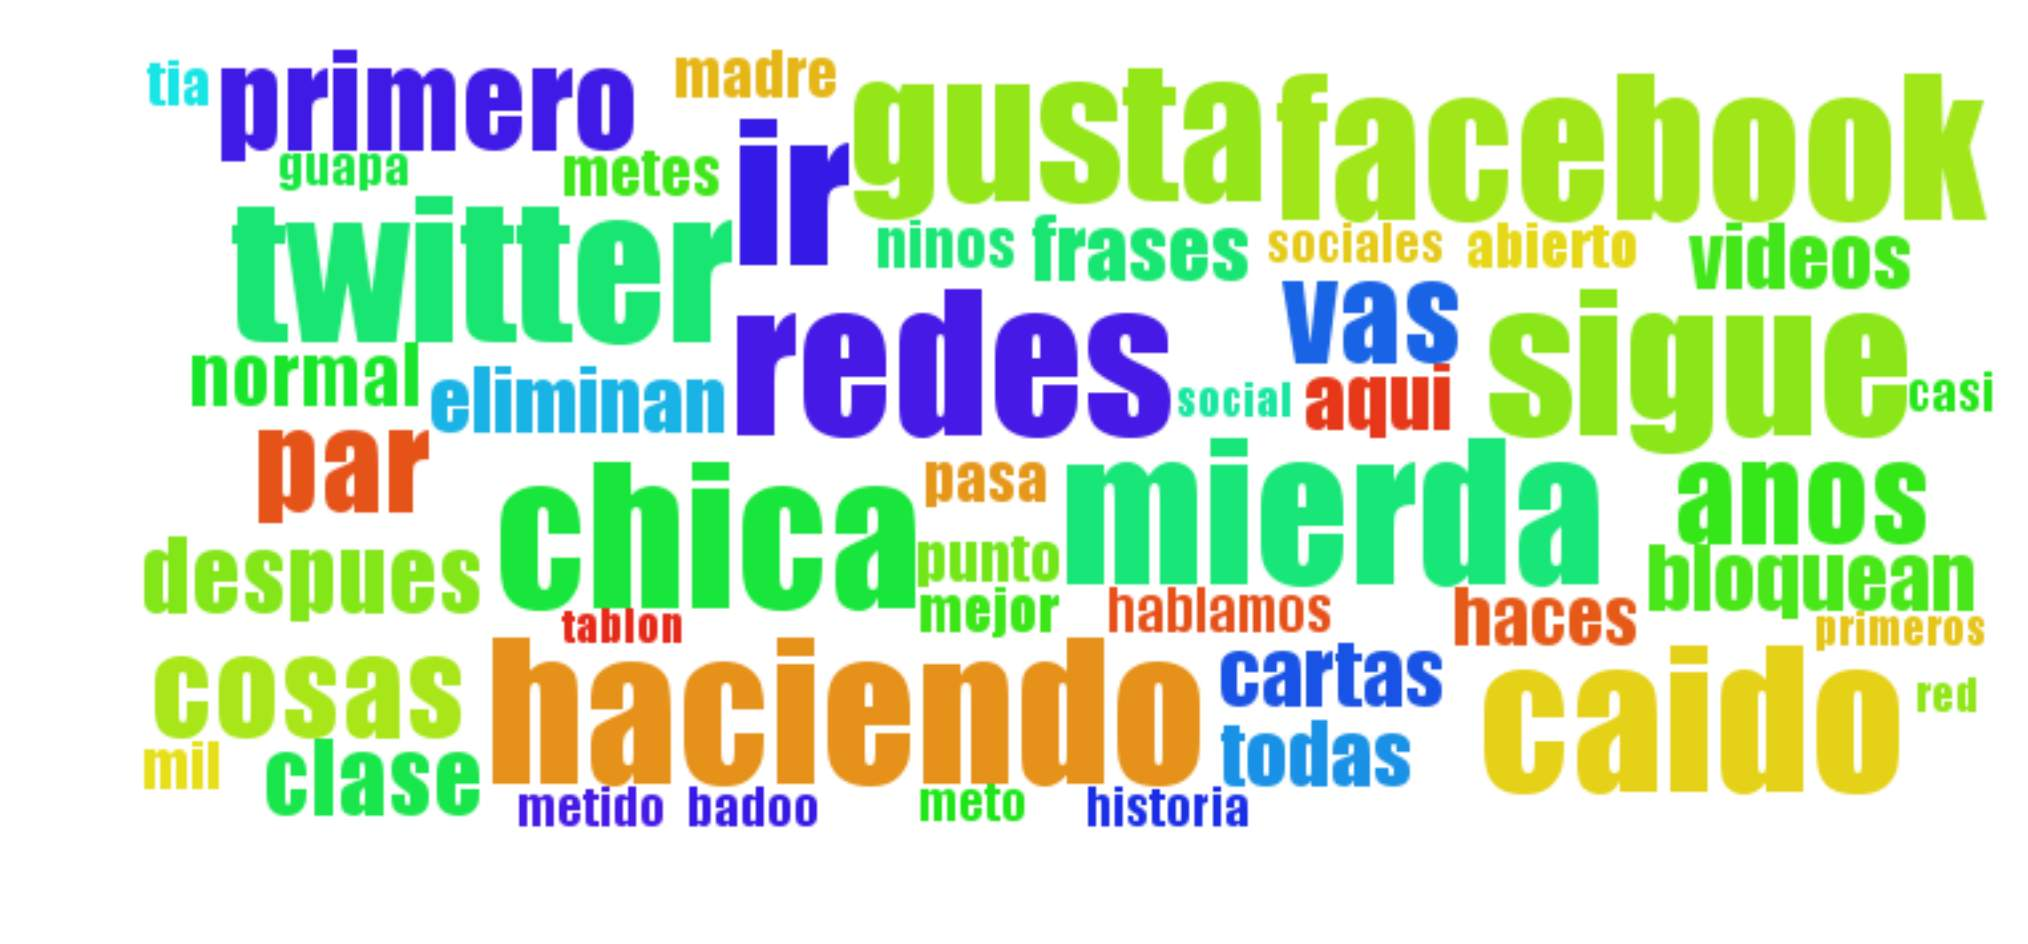
\includegraphics[width=\textwidth]{twitter_murcia/report_images/topic-02-wordcloud.jpg}
    \end{subfigure}
    \begin{subfigure}[b]{0.49\textwidth}
        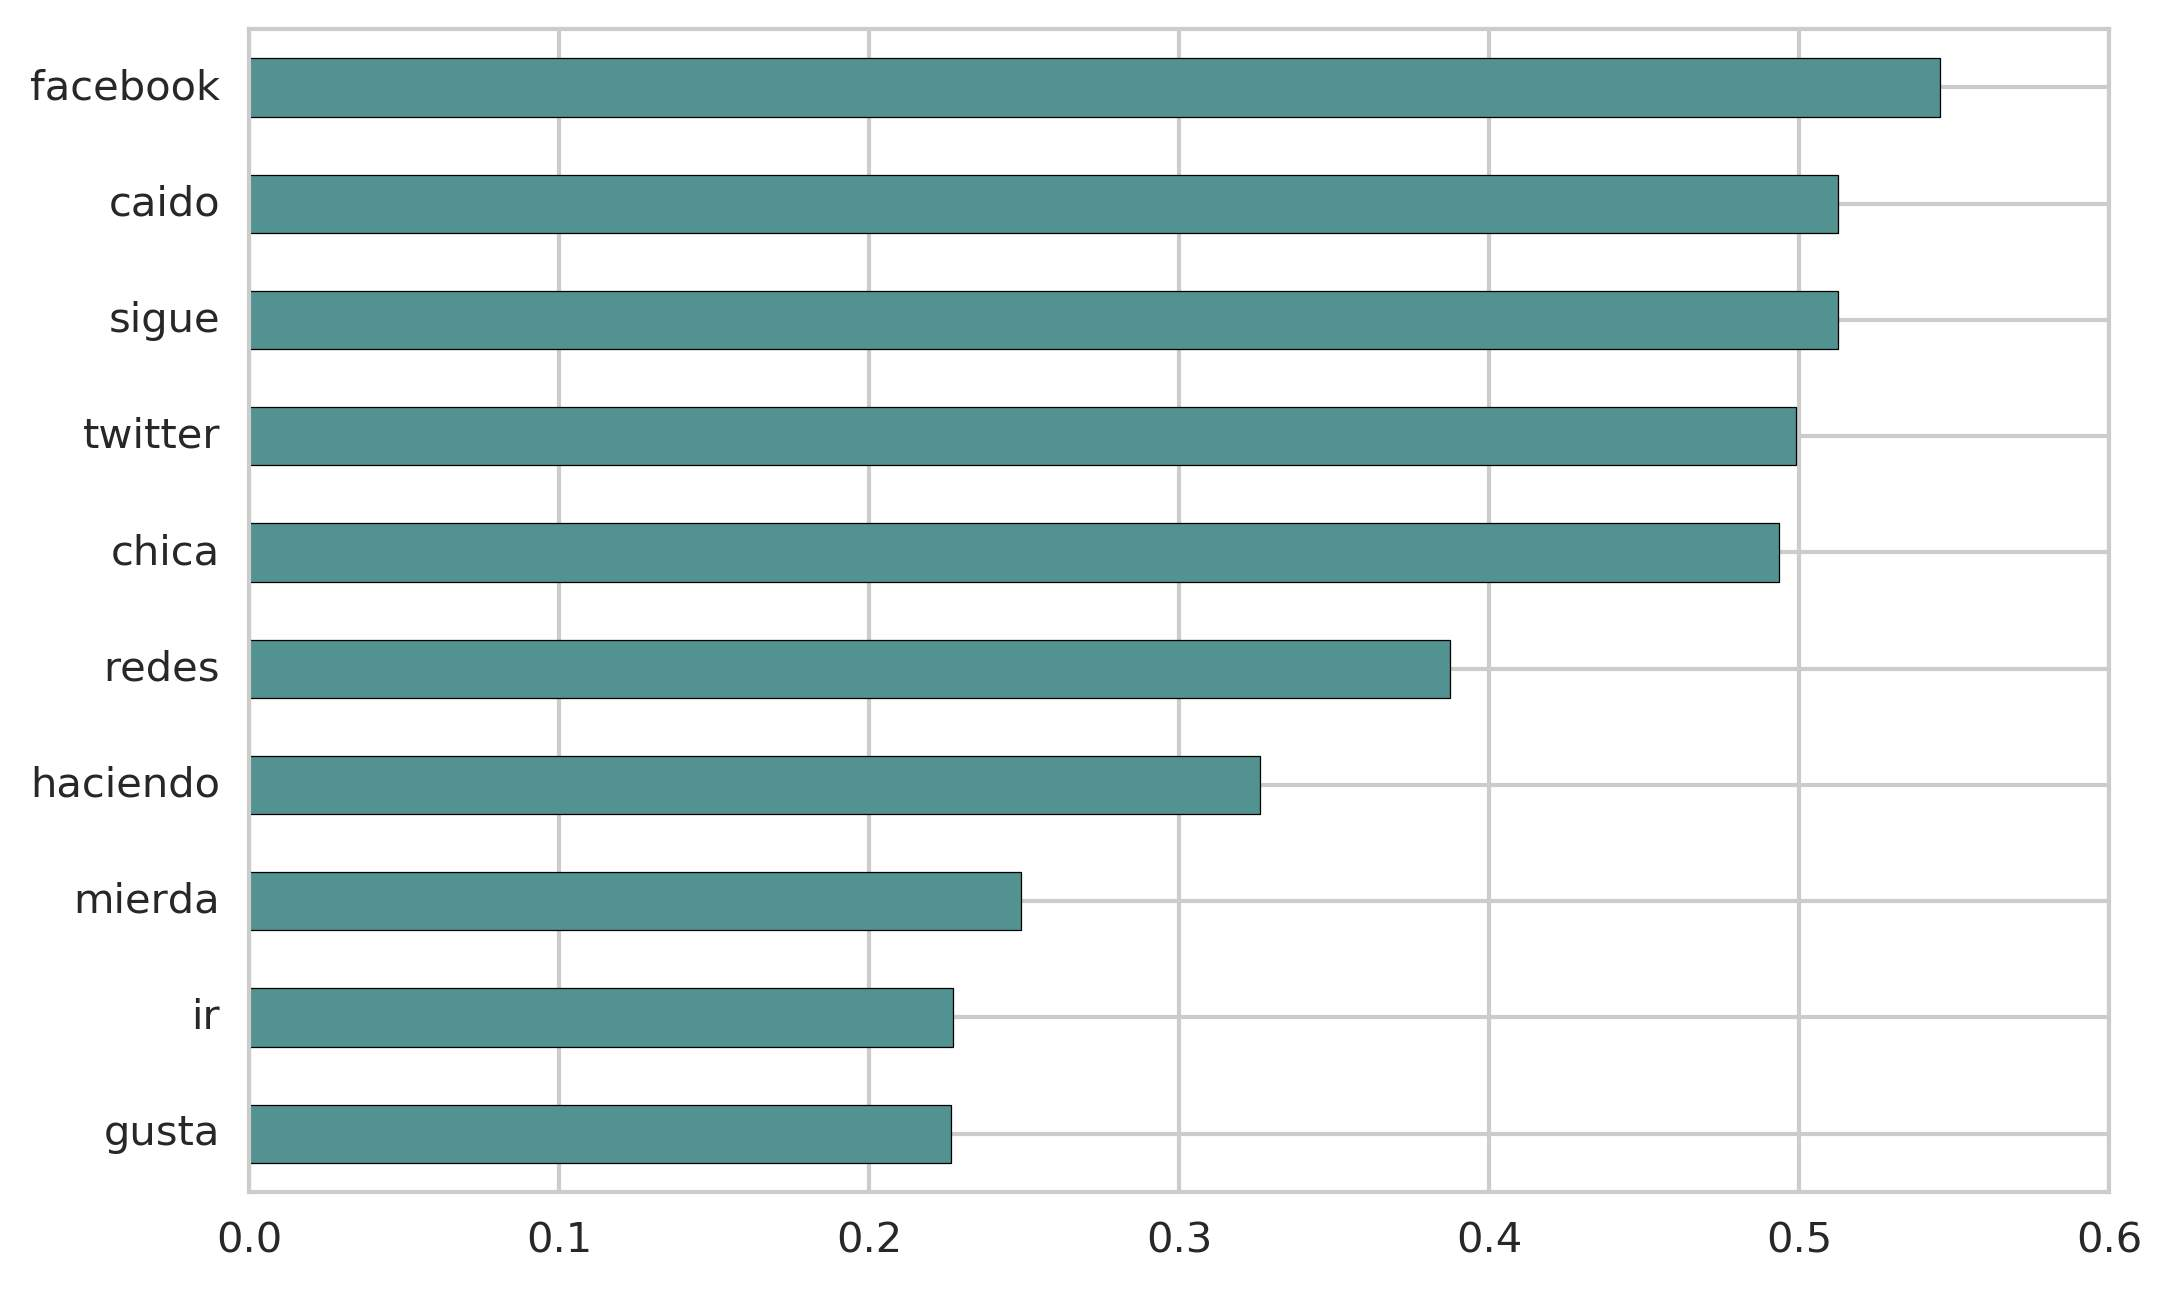
\includegraphics[width=\textwidth]{twitter_murcia/report_images/topic-02-terms.jpg}
    \end{subfigure}
\end{figure}

\begin{figure}[htbp!]
    \centering
    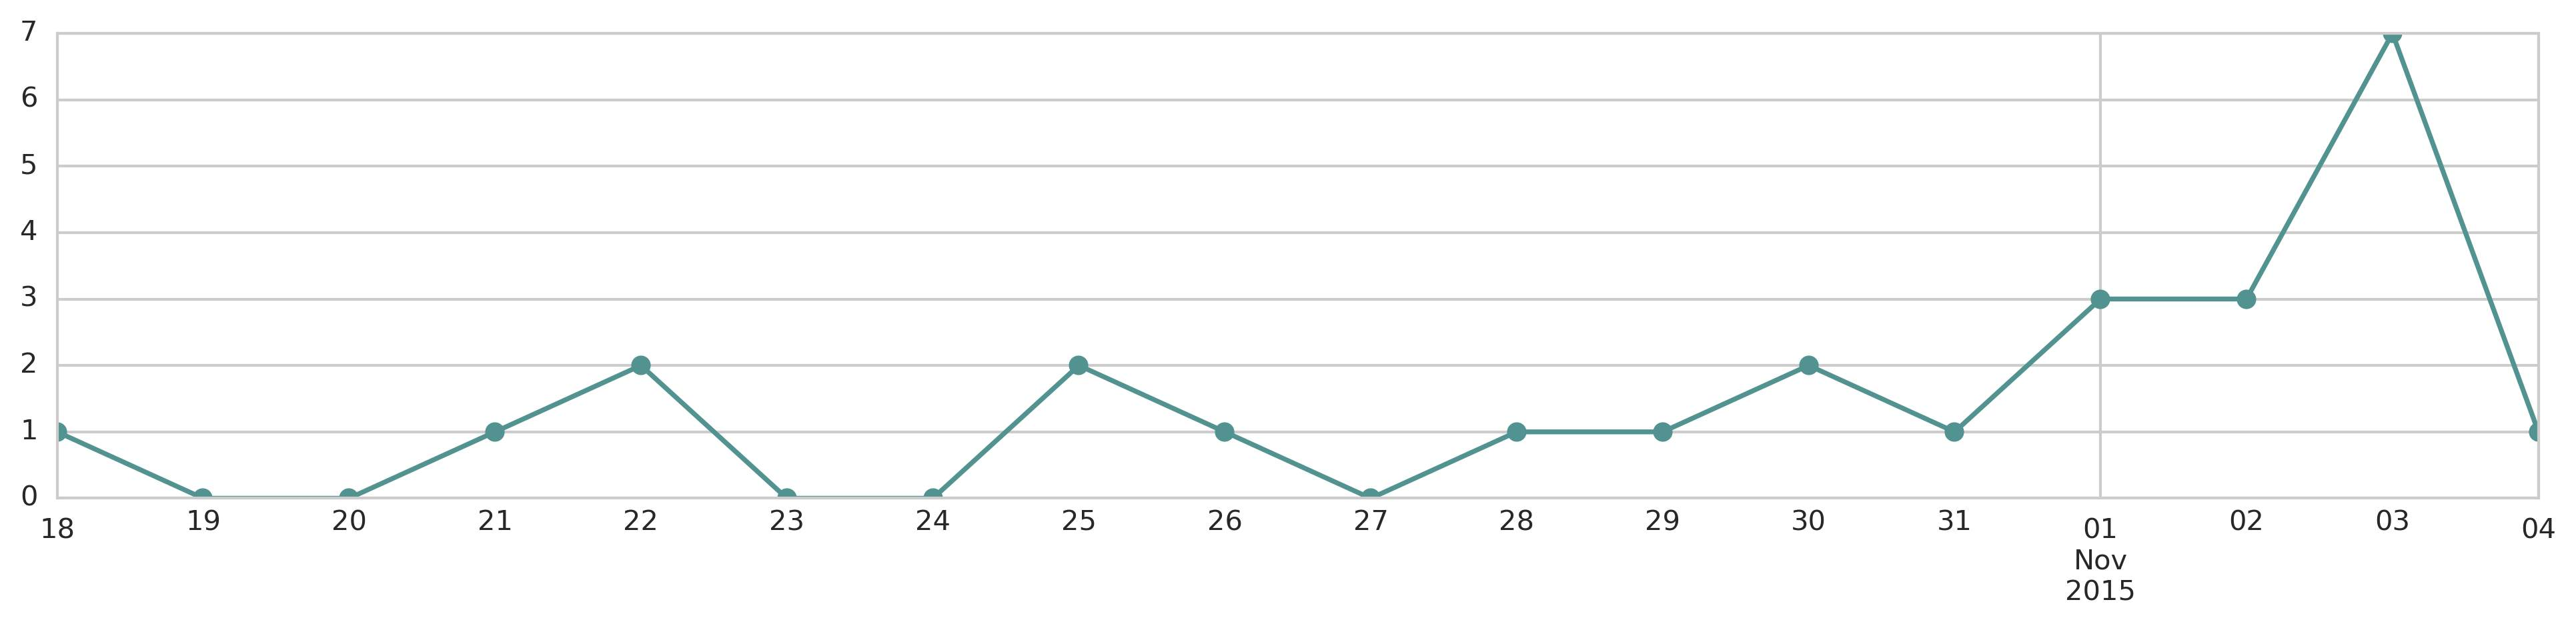
\includegraphics[width=\textwidth]{twitter_murcia/report_images/topic-02-timeseries.jpg}
\end{figure}

\rowcolors{2}{gray!25}{white}
\begin{longtable}{p{12.5cm}rr}
\toprule
Text & Count & Rel \\
\midrule
\endhead
\midrule
\multicolumn{3}{r}{{Continued on next page}} \\
\midrule
\endfoot

\bottomrule
\endlastfoot
RT @UnAIumno: Si una chica te sigue en Twitter, Facebook y Tuenti enhorabuena. HA CAÍDO EN TUS REDES. & 4 & 0.81 \\
Primero Tuenti emuló a Facebook. Y Twitter lo lleva haciendo un par de años. Mierda corazones de Me Gusta. & 1 & 0.47 \\
Twitter está haciendo lo que Tuenti, ir añadiendo cosas de Facebook hasta ser una copia. & 1 & 0.45 \\
RT @Pauvlychenko: Twitter está haciendo lo que Tuenti, ir añadiendo cosas de Facebook hasta ser una copia. & 1 & 0.45 \\
Tuenti muertisimo, twitter muriendo, vas despues facebook 😂 & 1 & 0.34 \\
RT @Juanfranmoya: Tuenti muertisimo, twitter muriendo, vas despues facebook 😂 & 2 & 0.34 \\
RT @xmoguri: @Whiskeyandfire\_ JAJAJAJAJAJ TUENTI 2008 O FACEBOOK ACTUAL & 1 & 0.26 \\
Compartir videos de mierda y frases tuenti sí. Ir a una clase de zumba a perder las mollas, no tanto. & 1 & 0.21 \\
A N T E S: Se rimpian cartas y fotob A H O R A: Te eliminan y bloquean en Twitter, Tuenti y Facebook. & 1 & 0.19 \\
RT @Oscar\_Prc: @srtagalicia Ahora que lo pienso, estuvieron a punto de echarme del instituto por acosar a una chica por Tuenti. & 1 & 0.17 \\
@khaledfth @mariiemrafii @OumaimaSH madre mía, sois muchos niños en Twitter, tuenti es vuetro sitio, esto es de mayores, ro7o far9o jarrti & 1 & 0.12 \\
RT @manal\_arba: @khaledfth @mariiemrafii @OumaimaSH madre mía, sois muchos niños en Twitter, tuenti es vuetro sitio, esto es de mayores, ro… & 1 & 0.12 \\
Twitter quedará como messenguer y tuenti. A la historia & 1 & 0.11 \\
@Diexiseks normal, Twitter es de mayores, no sé qué haces tú aquí. Lo tuyo es tuenti 😌 & 1 & 0.11 \\
He abierto tuenti después de unos años y qué maravilla :\_) & 1 & 0.10 \\
\begin{tabular}[c]{@{}l@{}}RT @CristiManson: @CristiCeldran. Y yo juuum\# \\ Tia escuchaaa, hablamos mejor por el tuenti? Esque el twitter este me va mas lento… u.u\end{tabular} & 1 & 0.09 \\
Cosas que se encuentran abriendo tuenti 😍 https://t.co/CFvsEoZz7w & 1 & 0.08 \\
@Brain\_Stew\_\_ de tuenti ni hablamos, no? & 1 & 0.01 \\
RT @Culii96: @Brain\_Stew\_\_ de tuenti ni hablamos, no? & 1 & 0.01 \\
RT @CristiCeldran: @CristiLoveDR Es que me he tenido que sesistalar el tuenti porque se me ha pillado, cuando se descarge, hablamos;) & 1 & 0.01 \\

\end{longtable}
\clearpage

\section{Topic 03}

\begin{figure}[htbp!]
    \centering
    \begin{subfigure}[b]{0.49\textwidth}
        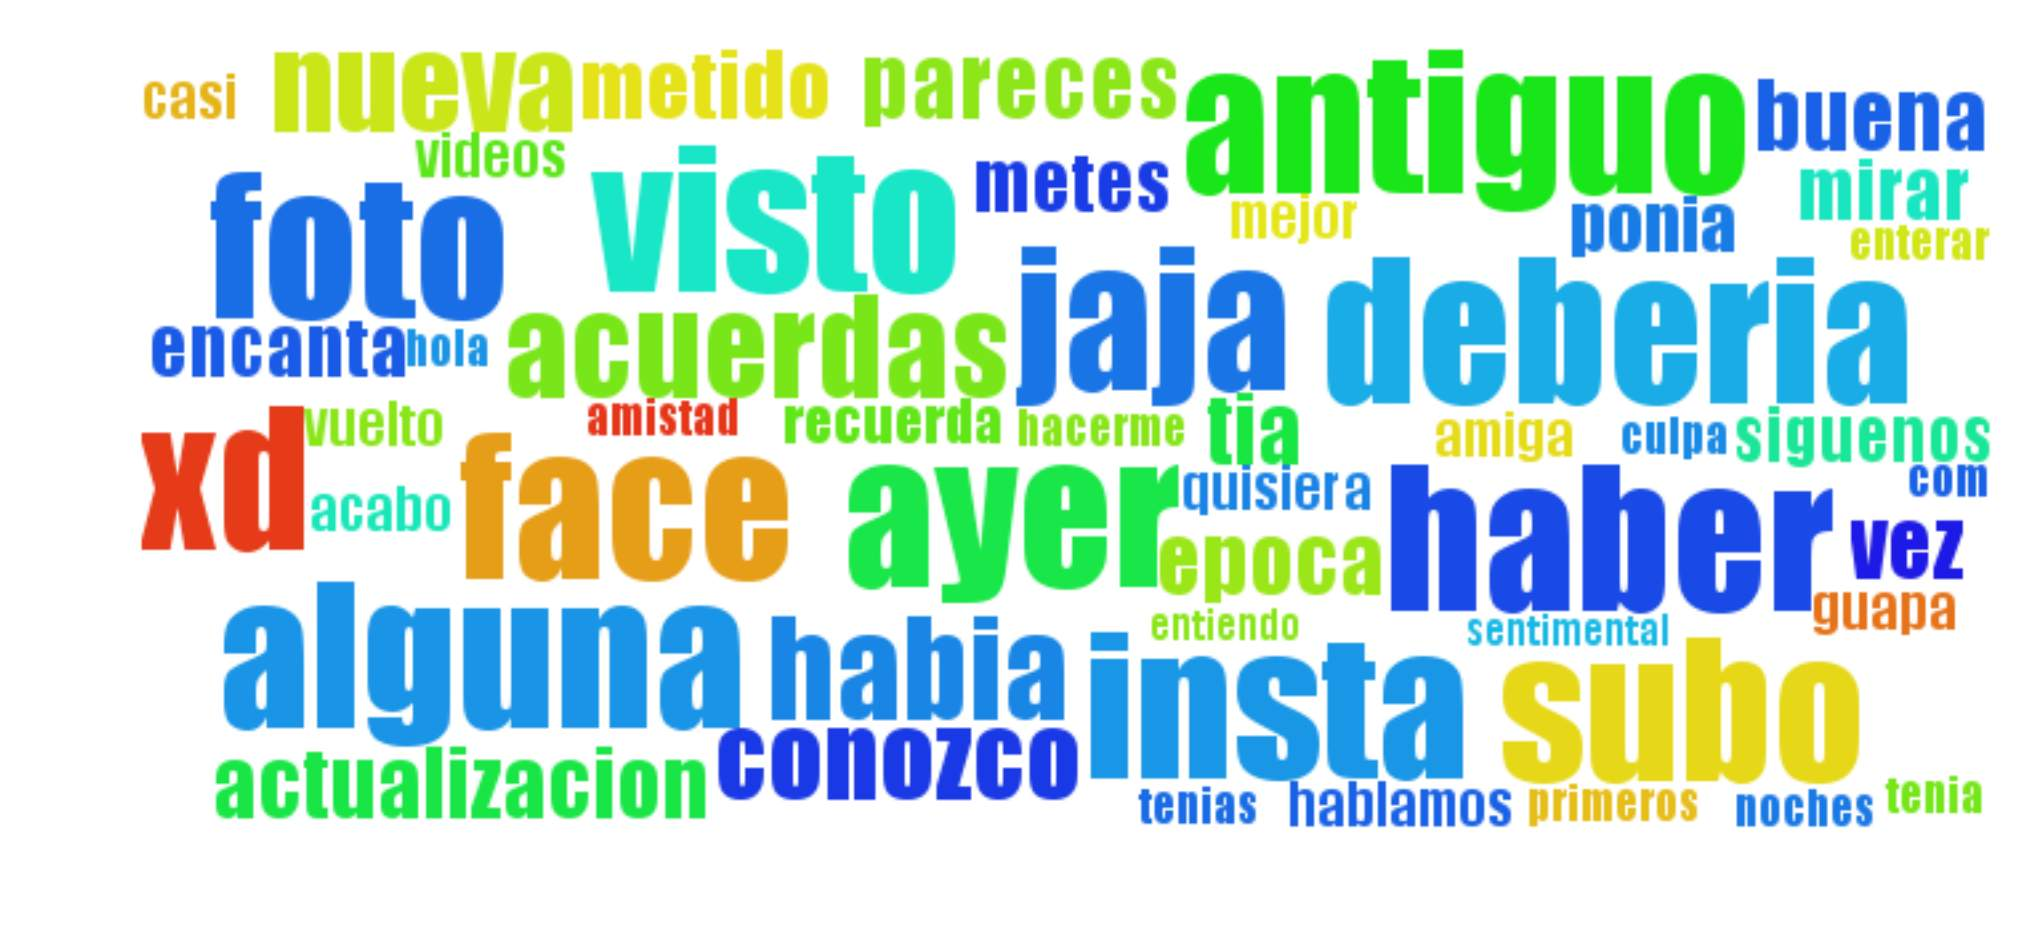
\includegraphics[width=\textwidth]{twitter_murcia/report_images/topic-03-wordcloud.jpg}
    \end{subfigure}
    \begin{subfigure}[b]{0.49\textwidth}
        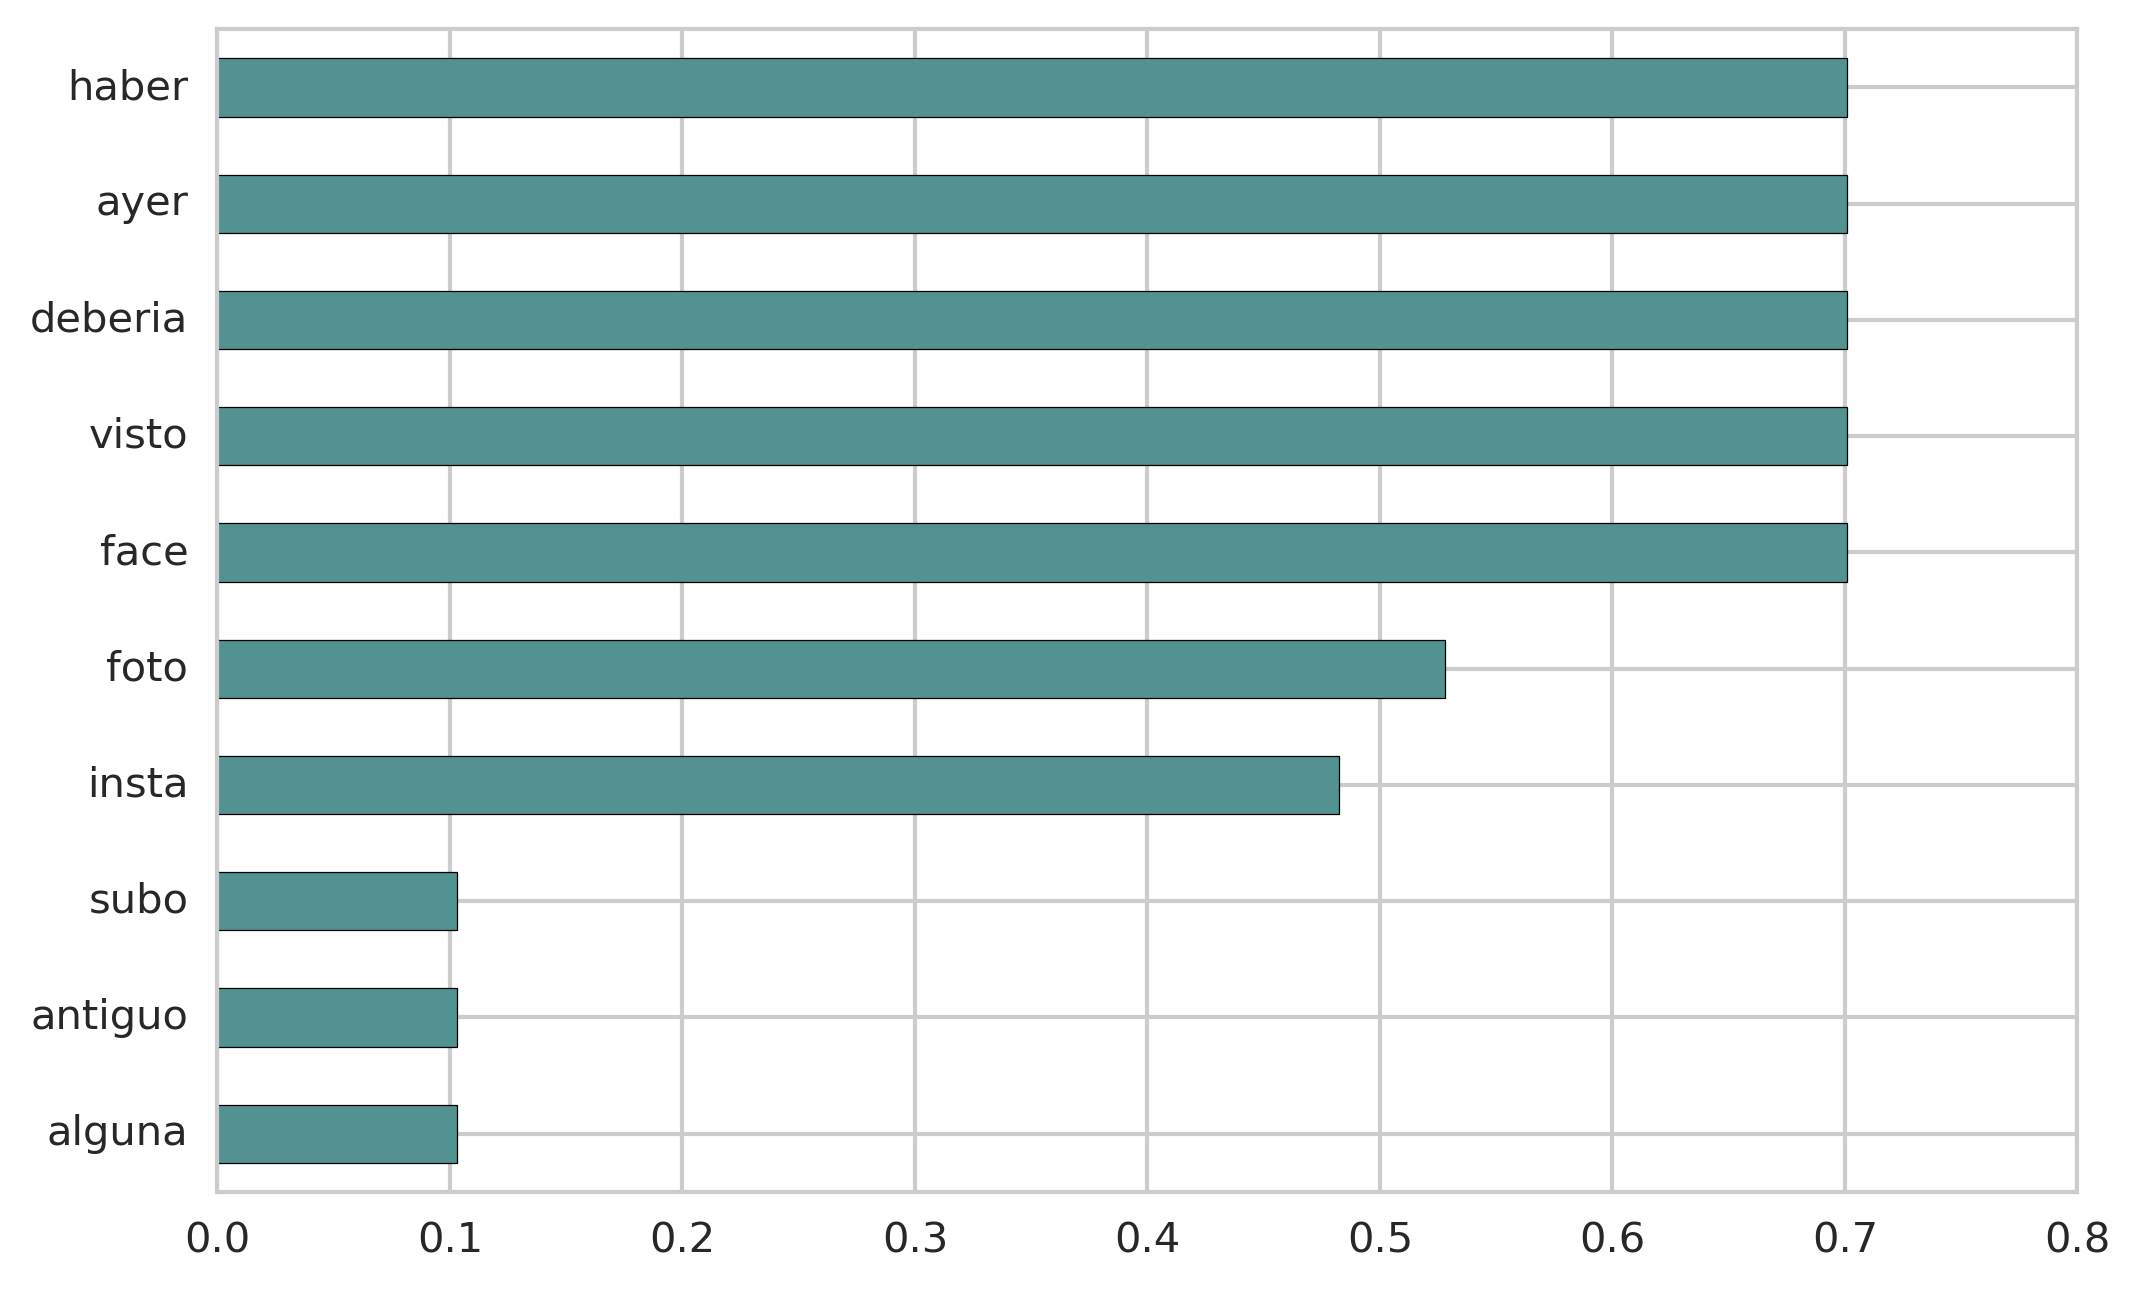
\includegraphics[width=\textwidth]{twitter_murcia/report_images/topic-03-terms.jpg}
    \end{subfigure}
\end{figure}

\begin{figure}[htbp!]
    \centering
    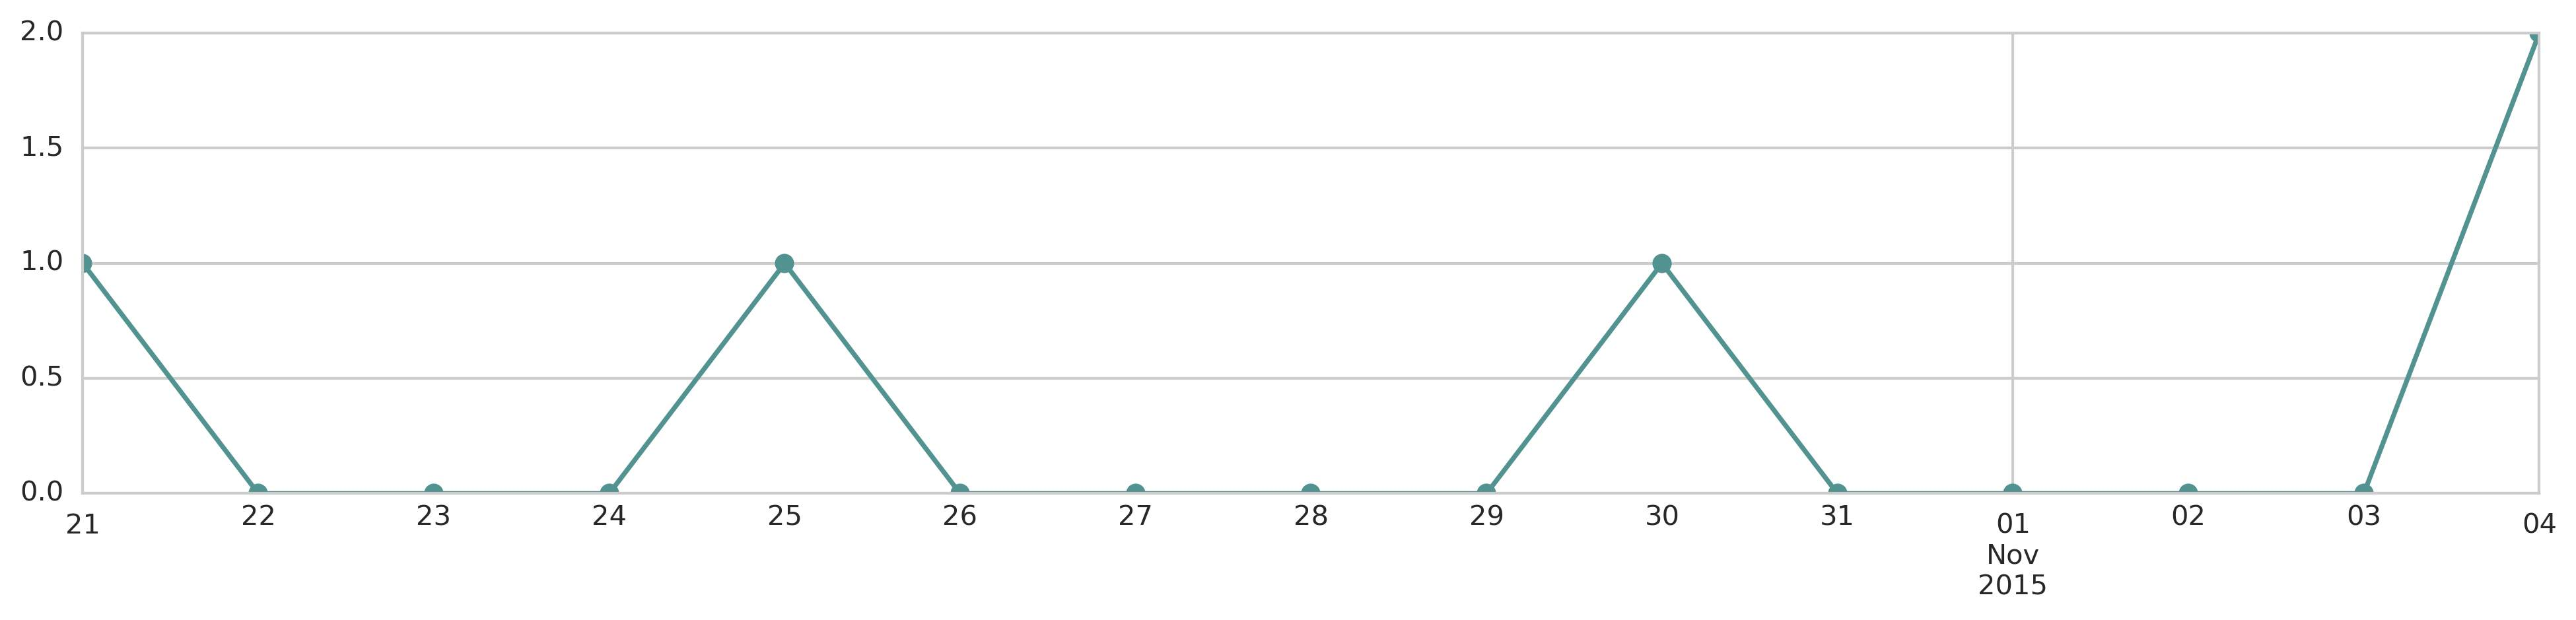
\includegraphics[width=\textwidth]{twitter_murcia/report_images/topic-03-timeseries.jpg}
\end{figure}

\rowcolors{2}{gray!25}{white}
\begin{longtable}{p{12.5cm}rr}
\toprule
Text & Count & Rel \\
\midrule
\endhead
\midrule
\multicolumn{3}{r}{{Continued on next page}} \\
\midrule
\endfoot

\bottomrule
\endlastfoot
Yo ayer deberia haber visto a andrés suarez y haberme echado una foto con el y subirla a insta face snap tuenti pero NO & 1 & 0.98 \\
¿Subo alguna foto de mi antiguo tuenti? AJAJJJJJJJJJJ & 1 & 0.17 \\
@LadyStarlight94 @MVR\_Campos Tiene por hay una foto vestido de mujer, te acuerdas Luis? la de Tuenti, sácala jajajaja & 1 & 0.15 \\
Cuando tenias peticiones de amistad en tuenti de tias 😆 & 1 & 0.00 \\
mmmmmmmmmmmme apetece hacerme autobullying, voy a tuenti. & 1 & 0.00 \\

\end{longtable}
\clearpage

\section{Topic 04}

\begin{figure}[htbp!]
    \centering
    \begin{subfigure}[b]{0.49\textwidth}
        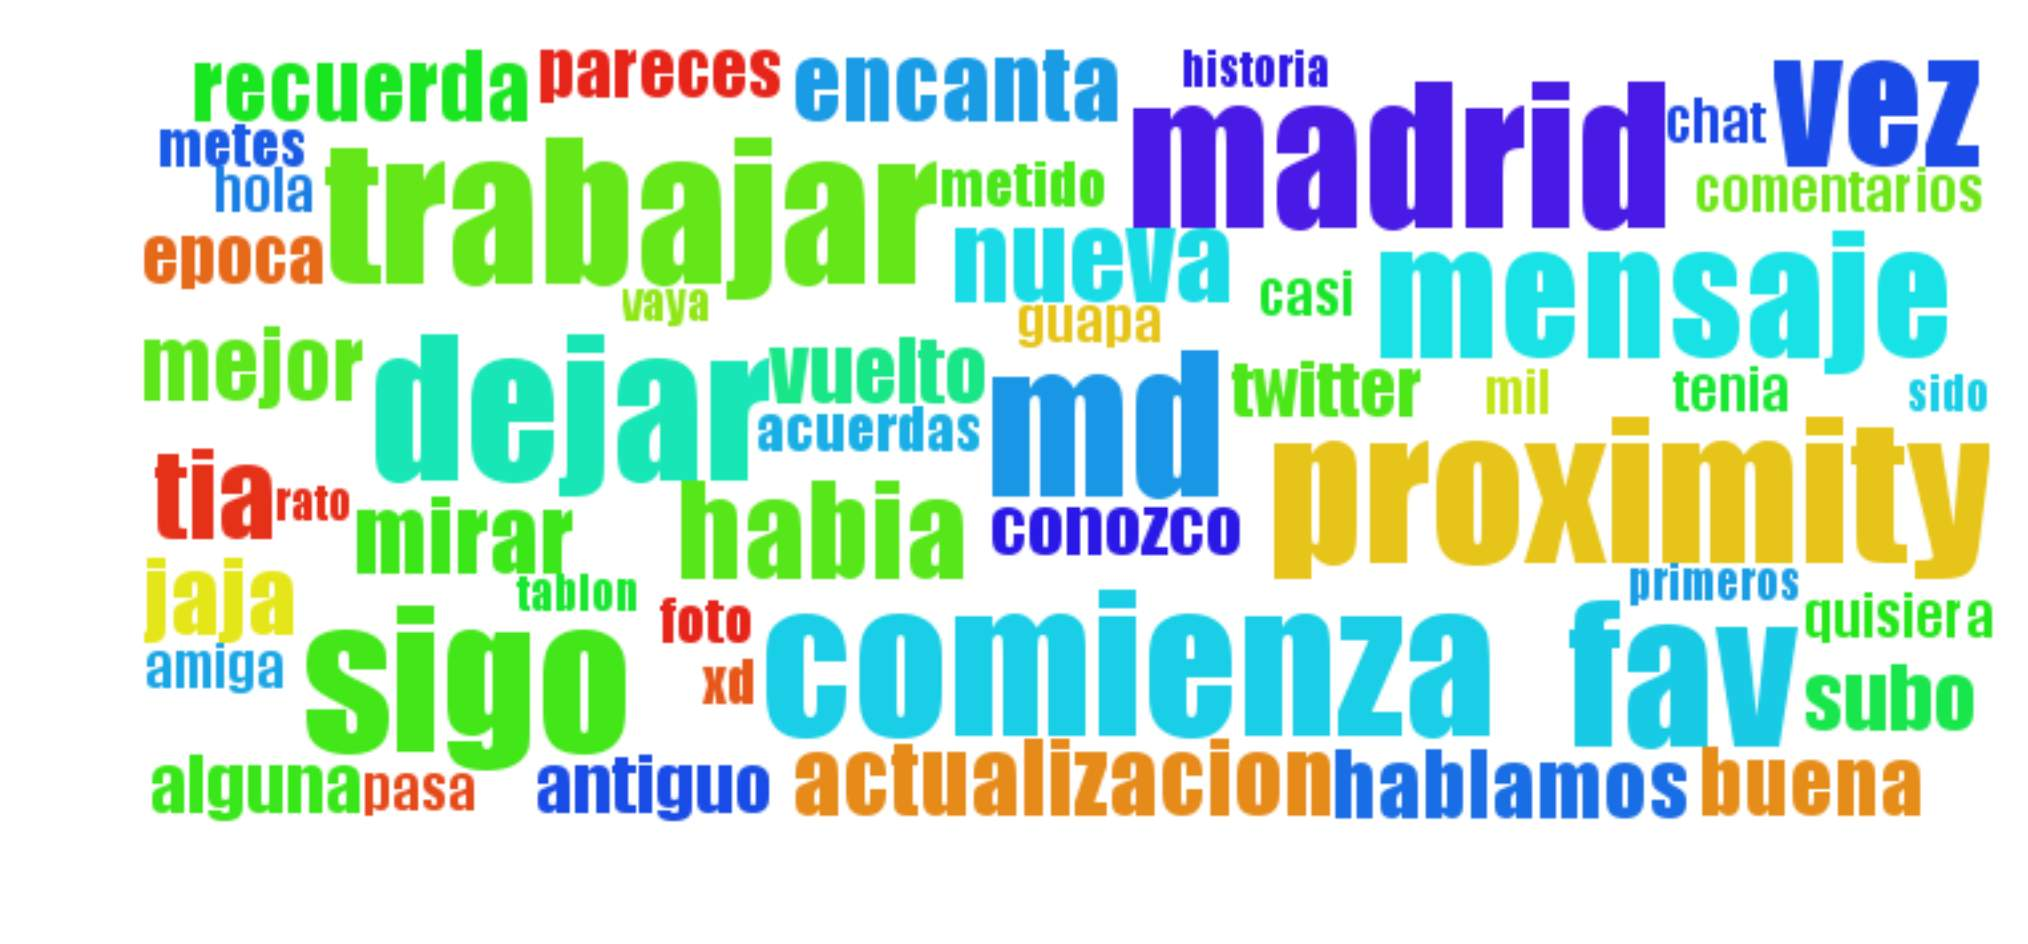
\includegraphics[width=\textwidth]{twitter_murcia/report_images/topic-04-wordcloud.jpg}
    \end{subfigure}
    \begin{subfigure}[b]{0.49\textwidth}
        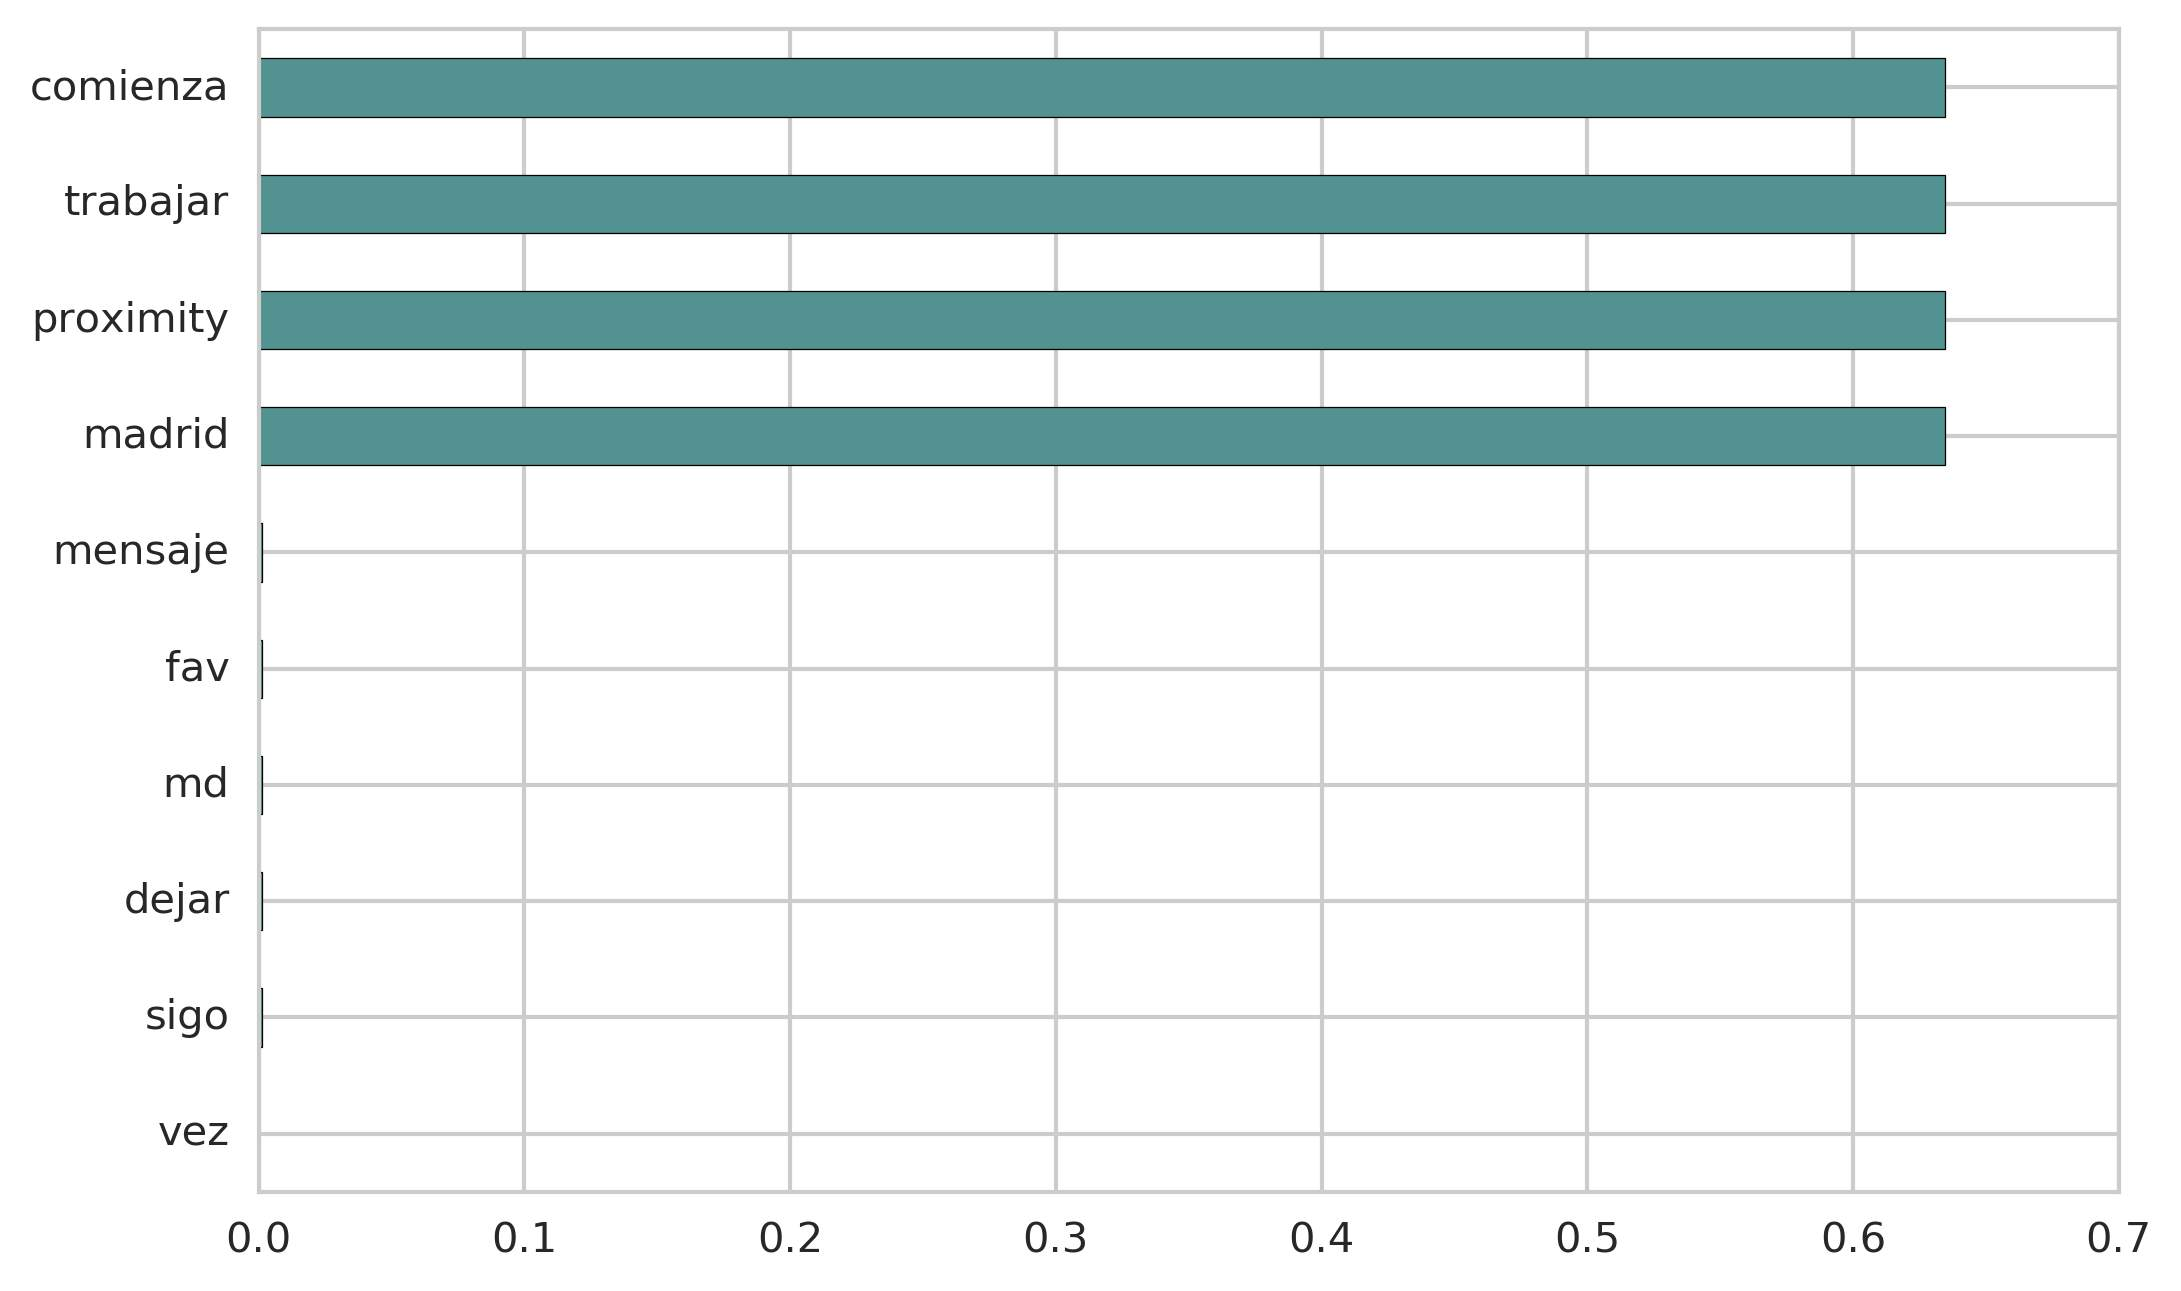
\includegraphics[width=\textwidth]{twitter_murcia/report_images/topic-04-terms.jpg}
    \end{subfigure}
\end{figure}

\begin{figure}[htbp!]
    \centering
    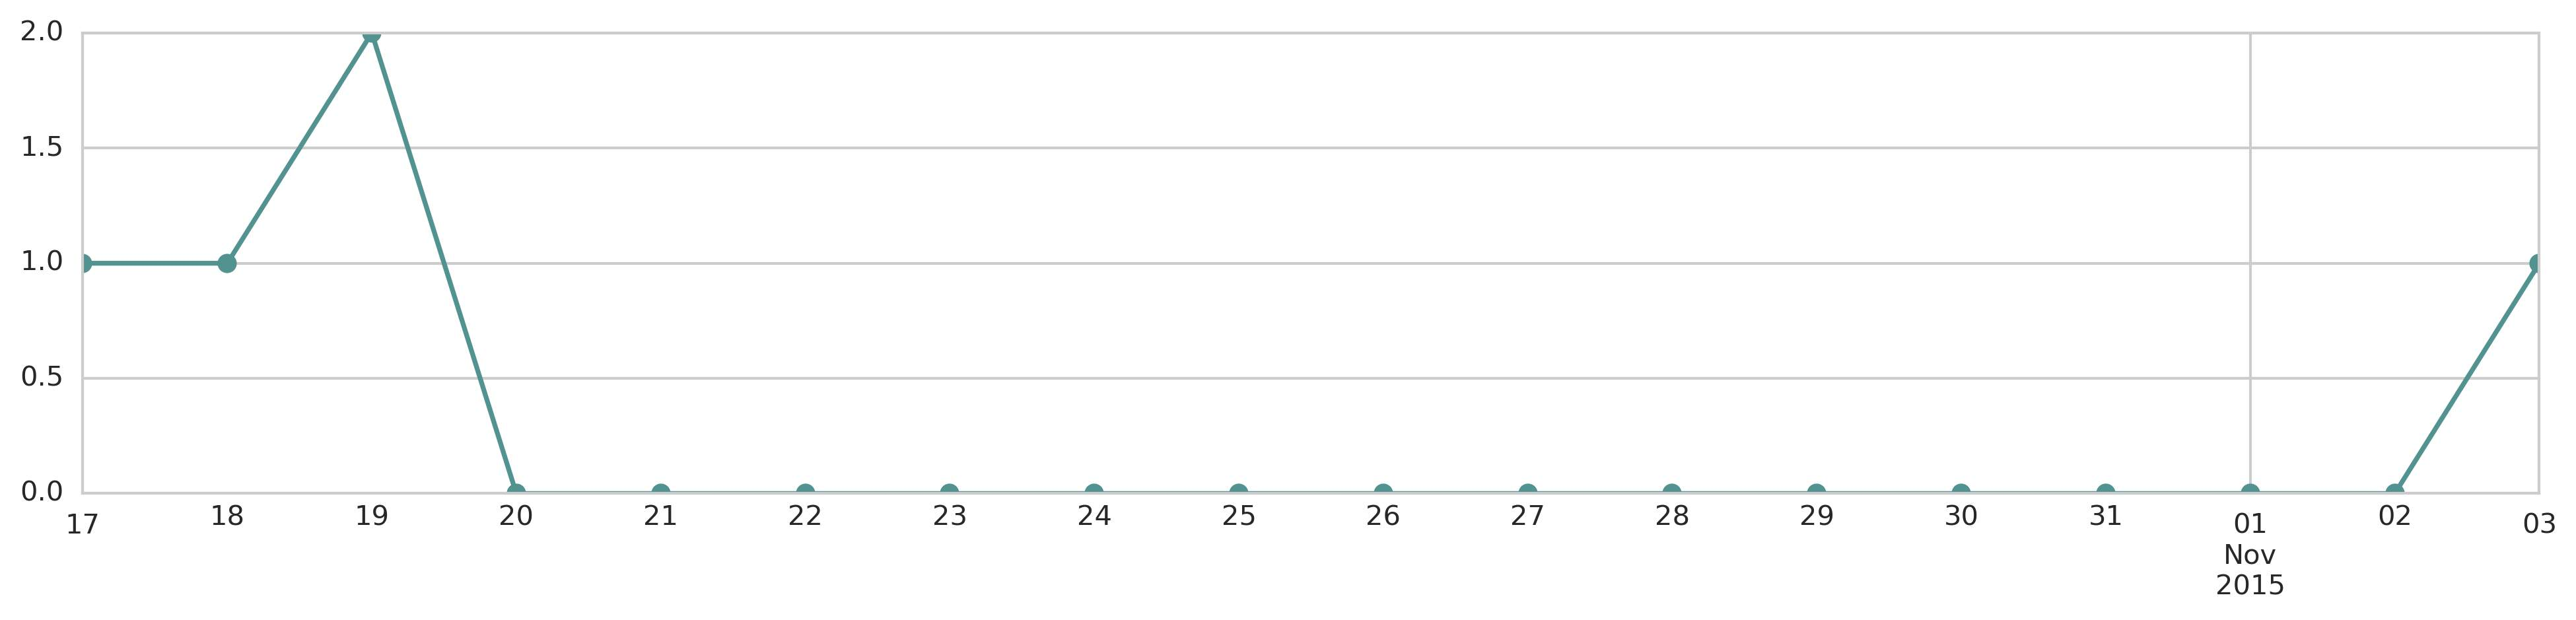
\includegraphics[width=\textwidth]{twitter_murcia/report_images/topic-04-timeseries.jpg}
\end{figure}

\rowcolors{2}{gray!25}{white}
\begin{longtable}{p{12.5cm}rr}
\toprule
Text & Count & Rel \\
\midrule
\endhead
\midrule
\multicolumn{3}{r}{{Continued on next page}} \\
\midrule
\endfoot

\bottomrule
\endlastfoot
Proximity Madrid comienza a trabajar para Tuenti:  http://t.co/INwVYyh6G5 \#comunicacion & 1 & 1.00 \\
Proximity Madrid comienza a trabajar para Tuenti:  http://t.co/3sBgMTwxoF \#publicidad & 1 & 1.00 \\
RT @Sergio\_Sala: Estás tú que voy a dejar de llamarle Fav cuando a los MD les sigo llamando Mensaje Privado, como en el Tuenti. & 1 & 0.00 \\
Tuenti troleandome a estas alturas. Vaya vaya... & 1 & 0.00 \\
¿Qué ha sido de Tuenti? & 1 & 0.00 \\

\end{longtable}
\clearpage

\section{Topic 05}

\begin{figure}[htbp!]
    \centering
    \begin{subfigure}[b]{0.49\textwidth}
        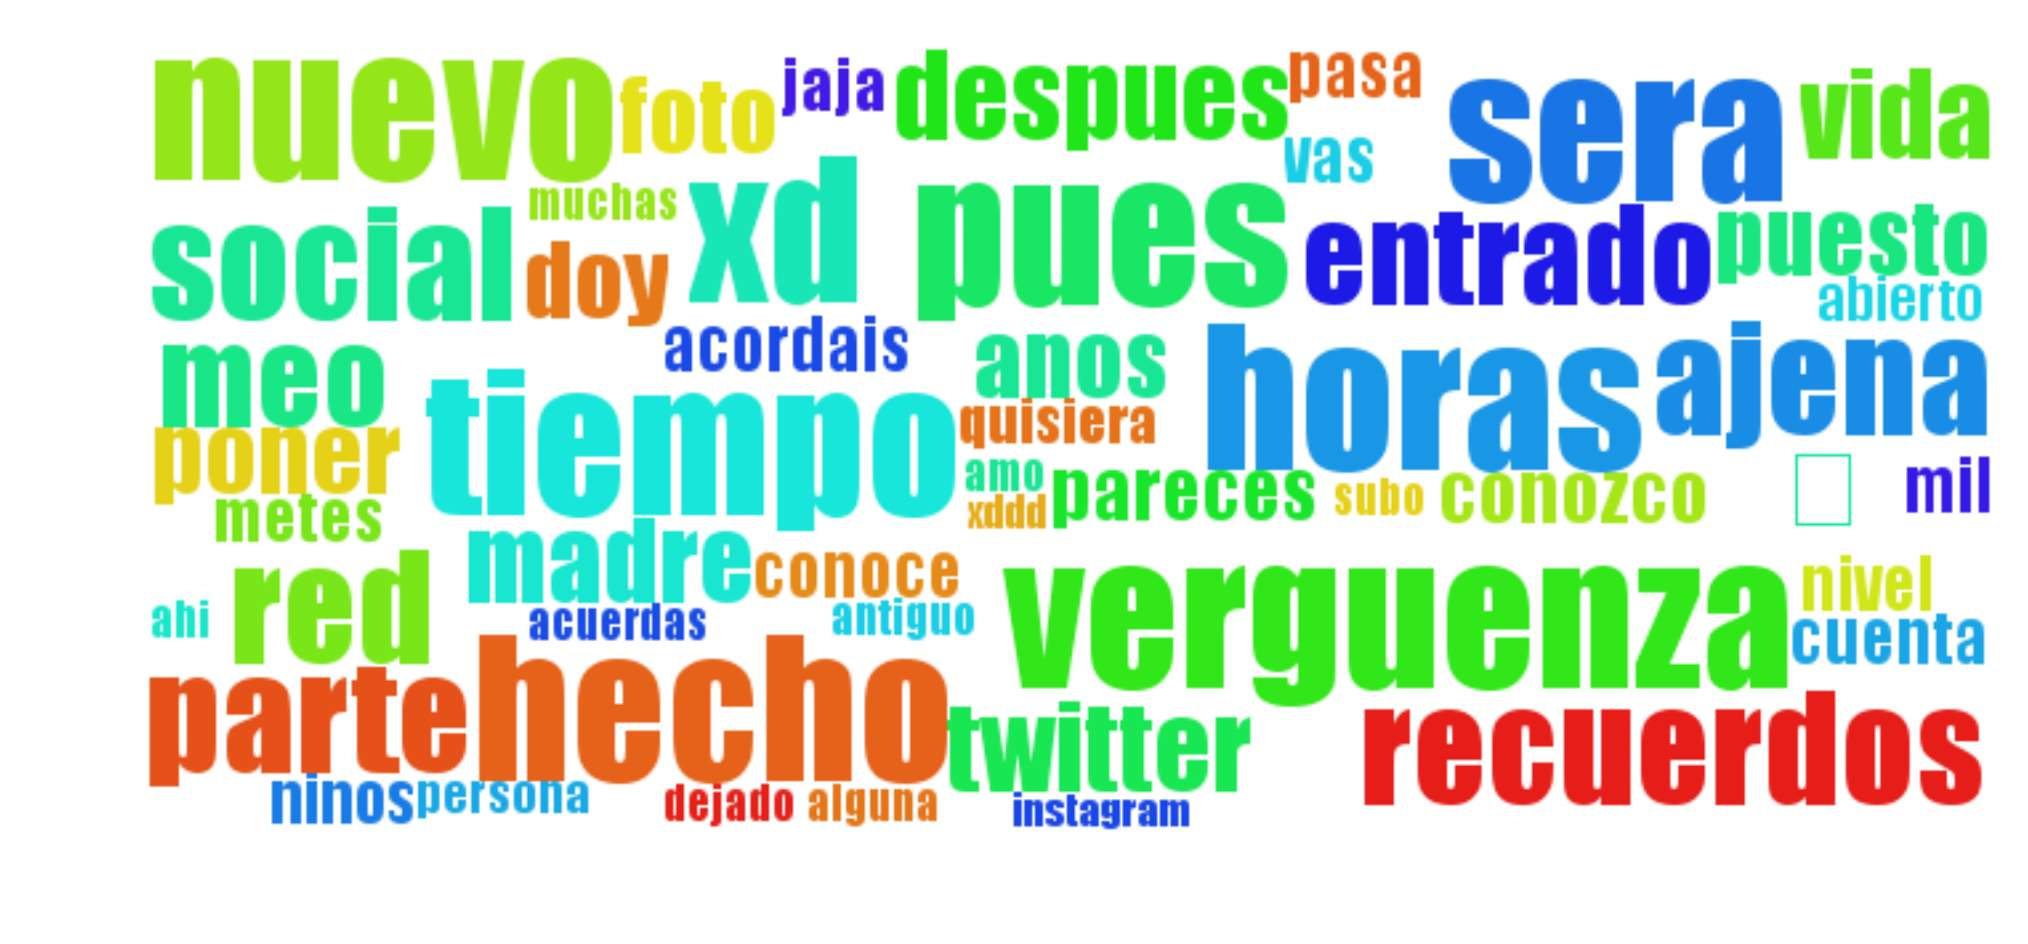
\includegraphics[width=\textwidth]{twitter_murcia/report_images/topic-05-wordcloud.jpg}
    \end{subfigure}
    \begin{subfigure}[b]{0.49\textwidth}
        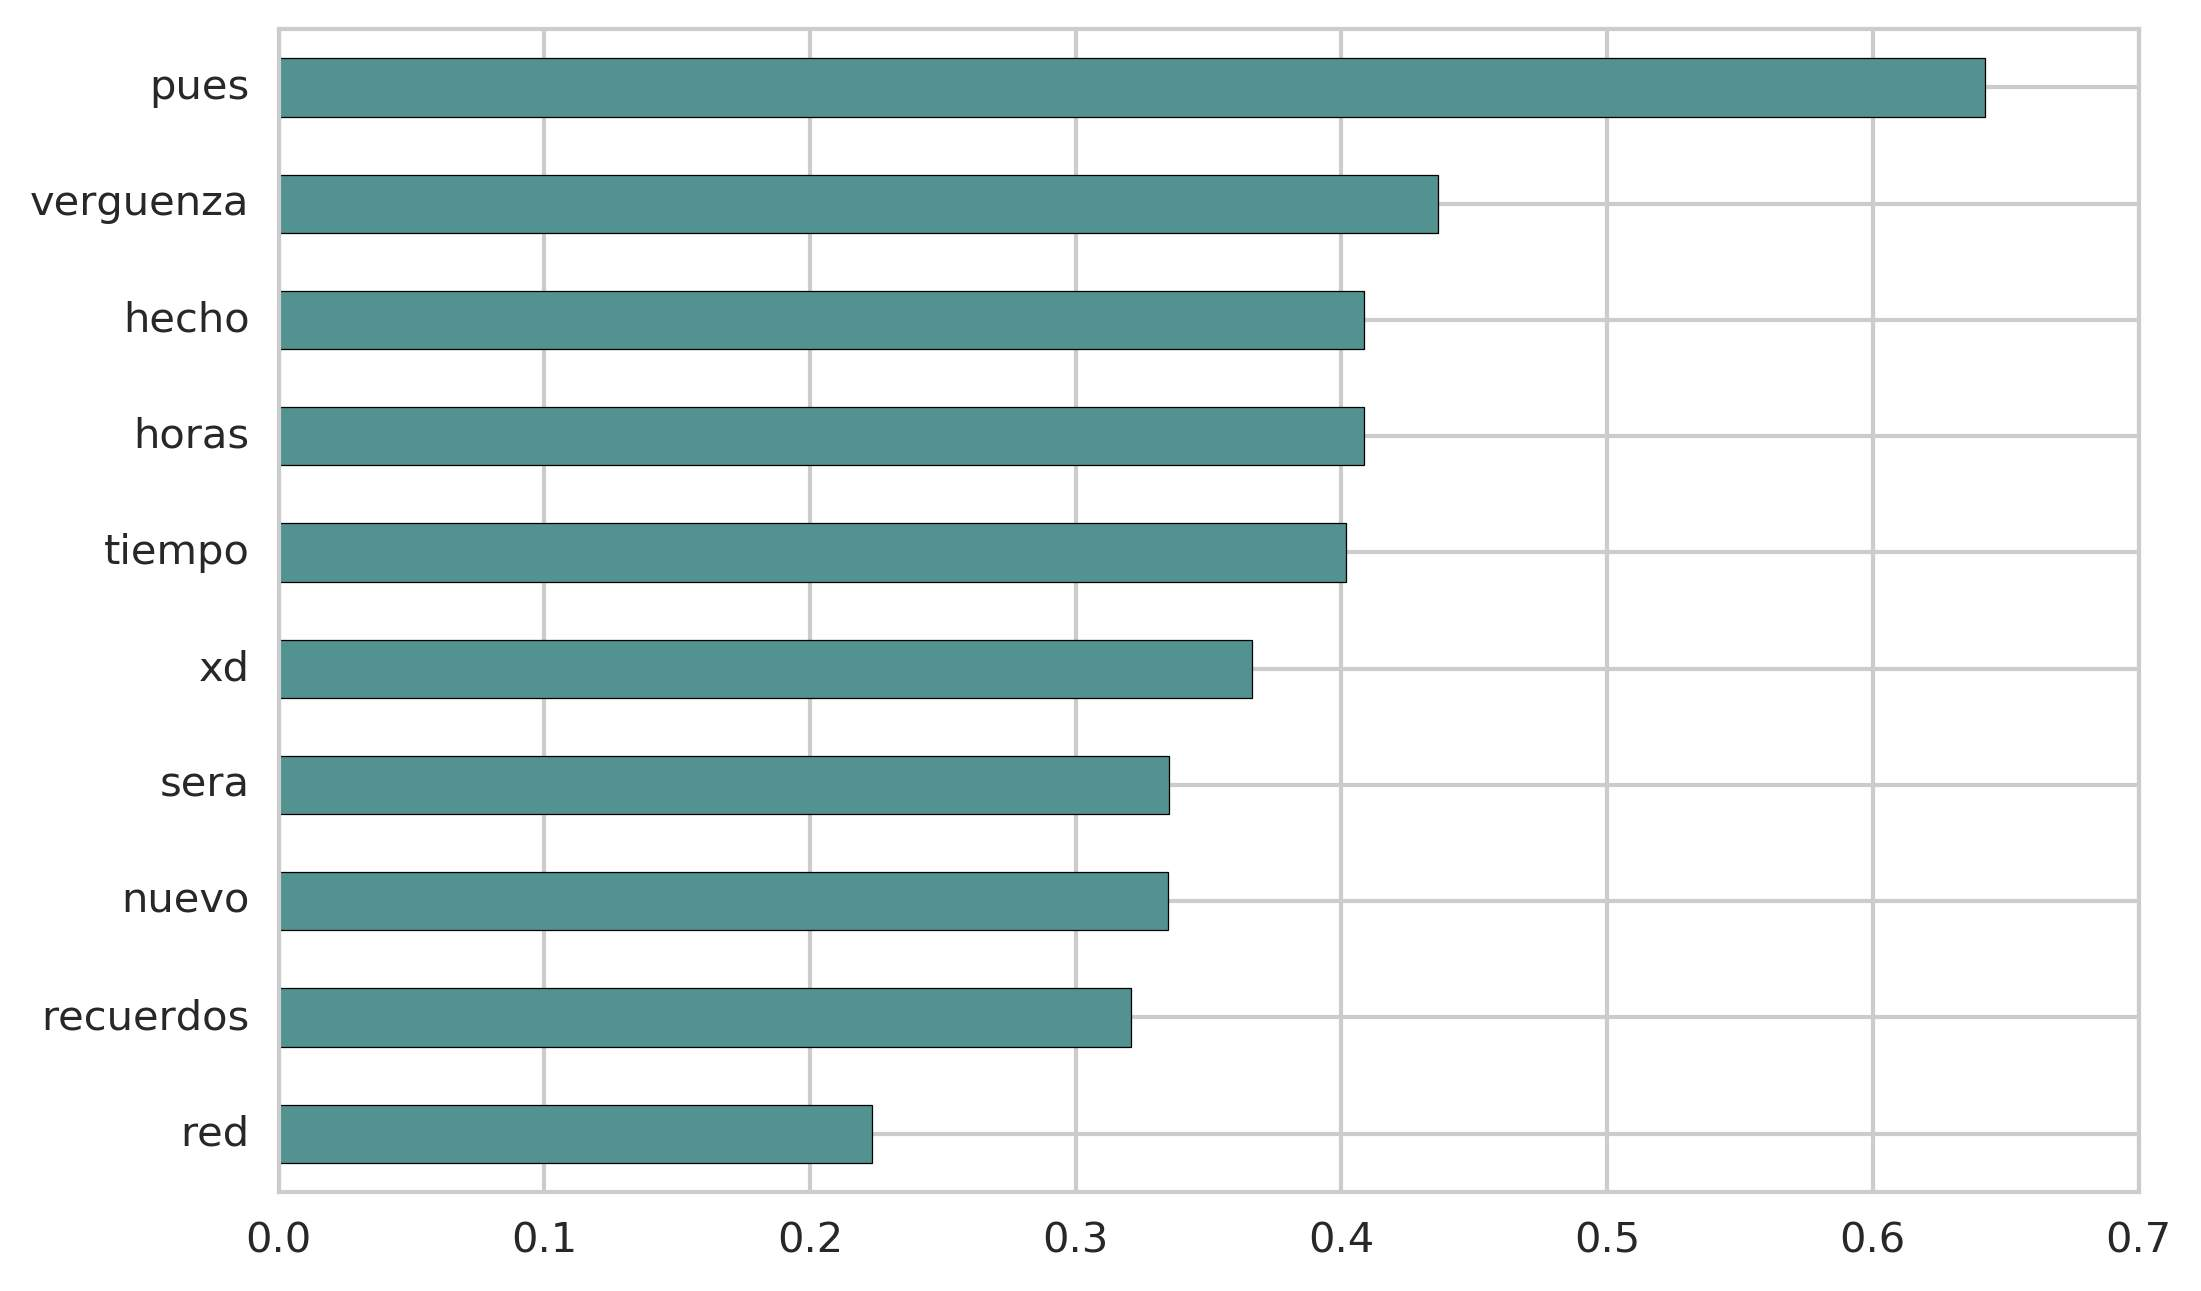
\includegraphics[width=\textwidth]{twitter_murcia/report_images/topic-05-terms.jpg}
    \end{subfigure}
\end{figure}

\begin{figure}[htbp!]
    \centering
    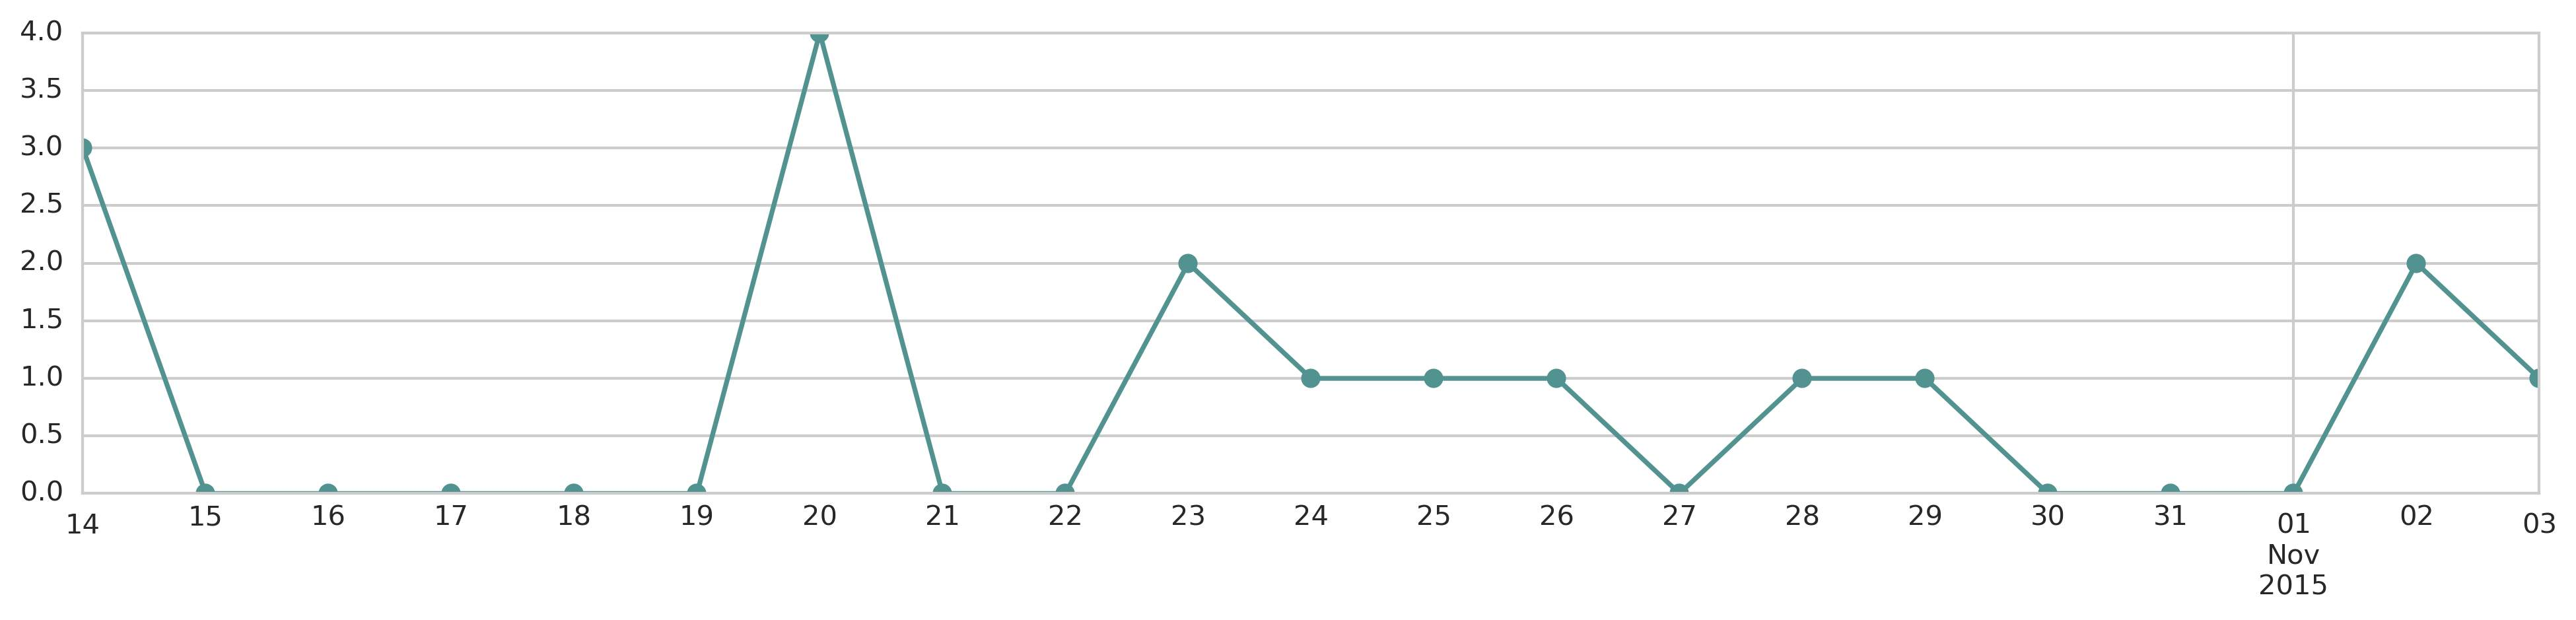
\includegraphics[width=\textwidth]{twitter_murcia/report_images/topic-05-timeseries.jpg}
\end{figure}

\rowcolors{2}{gray!25}{white}
\begin{longtable}{p{12.5cm}rr}
\toprule
Text & Count & Rel \\
\midrule
\endhead
\midrule
\multicolumn{3}{r}{{Continued on next page}} \\
\midrule
\endfoot

\bottomrule
\endlastfoot
\begin{tabular}[c]{@{}l@{}}¿Recordáis que nos da vergüenza que recuerden o miren lo que tenemos en Tuenti?  \\  \\ Pues recordad, en un tiempo, Twitter será el nuevo Tuenti.\end{tabular} & 1 & 0.65 \\
Pues no le he tirado horas al Backyard Monsters en tuenti, de hecho me conectaba sólo para eso xd & 1 & 0.63 \\
RT @\_FinchD: Pues no le he tirado horas al Backyard Monsters en tuenti, de hecho me conectaba sólo para eso xd & 1 & 0.63 \\
¿La red social de las indirectas?Antes estas se ponían en el estado de tuenti.Y eran indirectas pues...directas.Bastante MUCHO.Que recuerdos & 1 & 0.47 \\
RT @lessslove\_: a parte de verguenza ajena, tuenti me da muchos recuerdos bonitos 😂 & 1 & 0.39 \\
RT @roeln\_\_: me meo porque he entrado en tuenti después de todo este tiempo y next a mi vida & 1 & 0.31 \\
RT @ProfesorFuck: Quitar los FAVs en twitter solo es el comienzo para que la red social acabe como tuenti & 1 & 0.24 \\
De foto tuenti a selfie xd & 1 & 0.22 \\
RT @ph0enixx\_: De foto tuenti a selfie xd & 2 & 0.22 \\
RT @LoLSanlucar: Mi madre y yo nos hemos puesto a ver fotos de chicas en Tuenti para decidir como queremos poner el baño nuevo. & 1 & 0.17 \\
RT @ProudOfBiebeer: ¿os acordáis del tuenti? Que recuerdos... & 1 & 0.15 \\
@SrtoDany te conozco desde la era Tuenti xd Y me pareces muy puti. jejejejjee & 1 & 0.14 \\
Y eso es lo que pasa cuando te metes en tuenti después de mil años. & 1 & 0.10 \\
@levsad quiero su tuenti & 1 & 0.00 \\
RT @Vetacation: @levsad quiero su tuenti & 1 & 0.00 \\
RT @sebasmuriel: .. mi pasión, Tuenti, a tope !! .. https://t.co/OwBJ7riffC https://t.co/uYOx5FTMYA & 1 & 0.00 \\

\end{longtable}
\clearpage

\section{Topic 06}

\begin{figure}[htbp!]
    \centering
    \begin{subfigure}[b]{0.49\textwidth}
        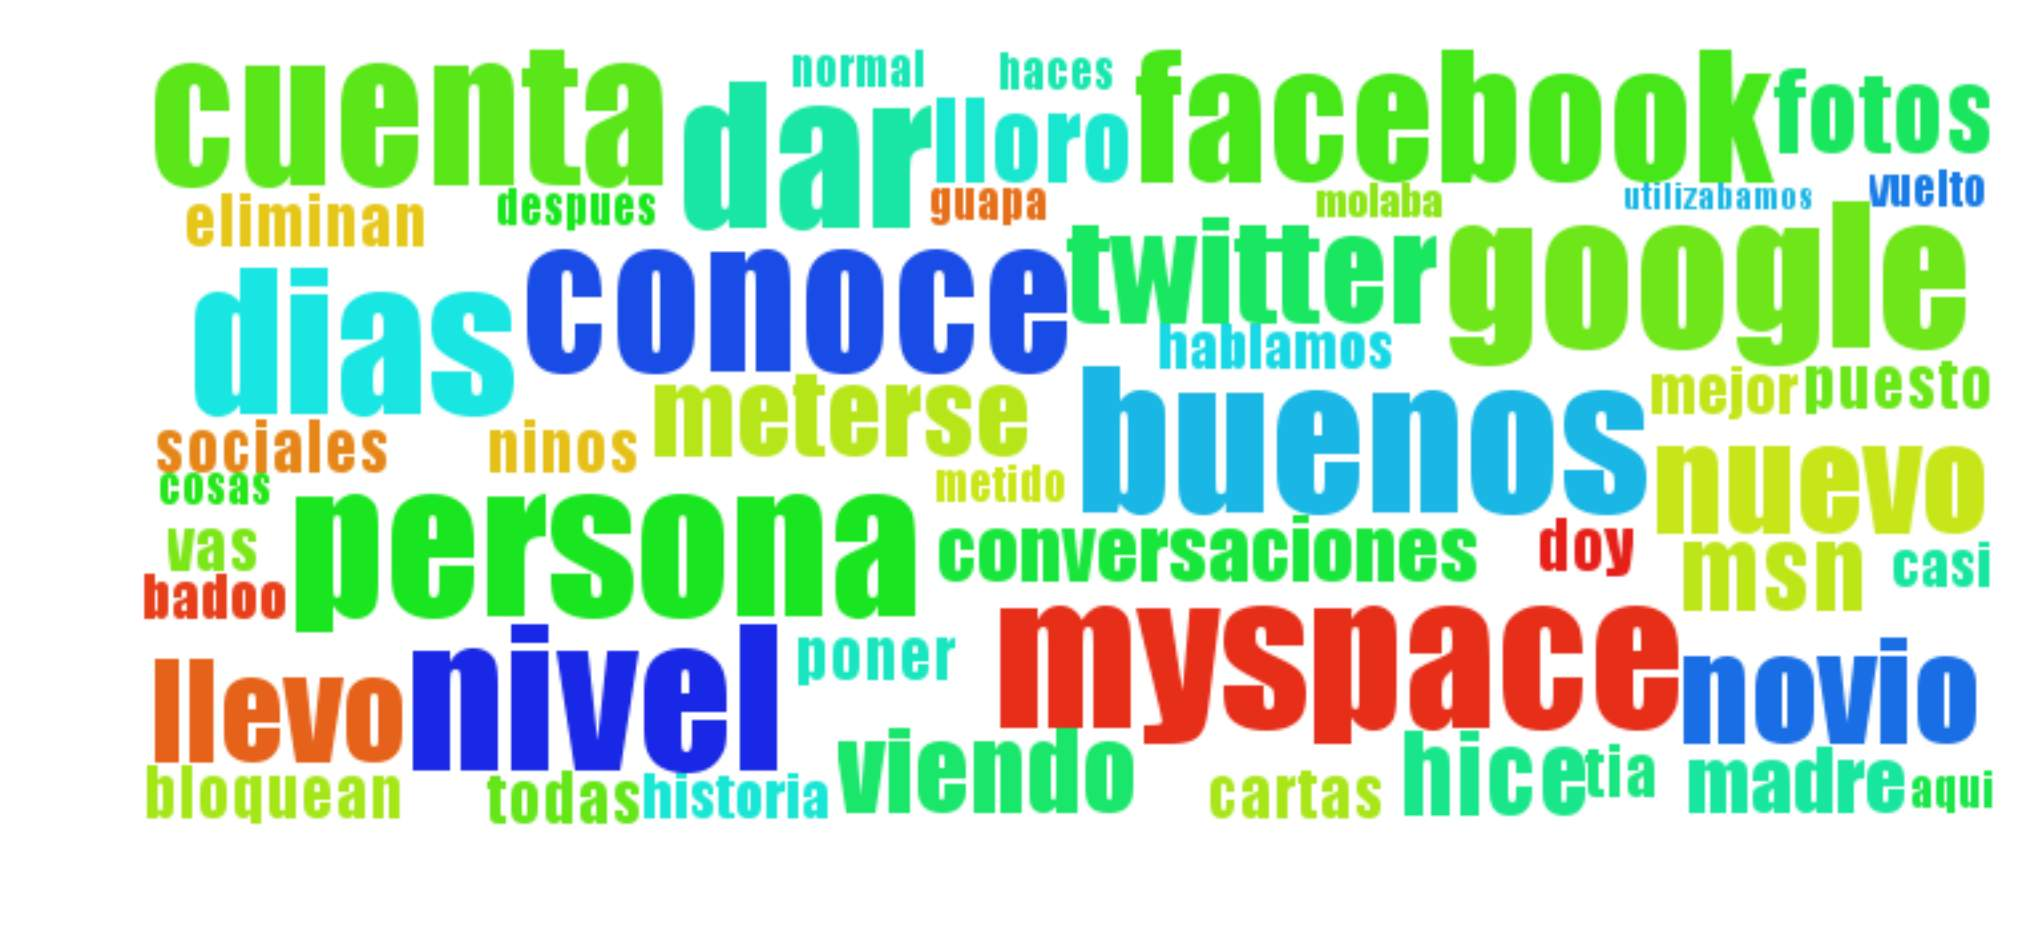
\includegraphics[width=\textwidth]{twitter_murcia/report_images/topic-06-wordcloud.jpg}
    \end{subfigure}
    \begin{subfigure}[b]{0.49\textwidth}
        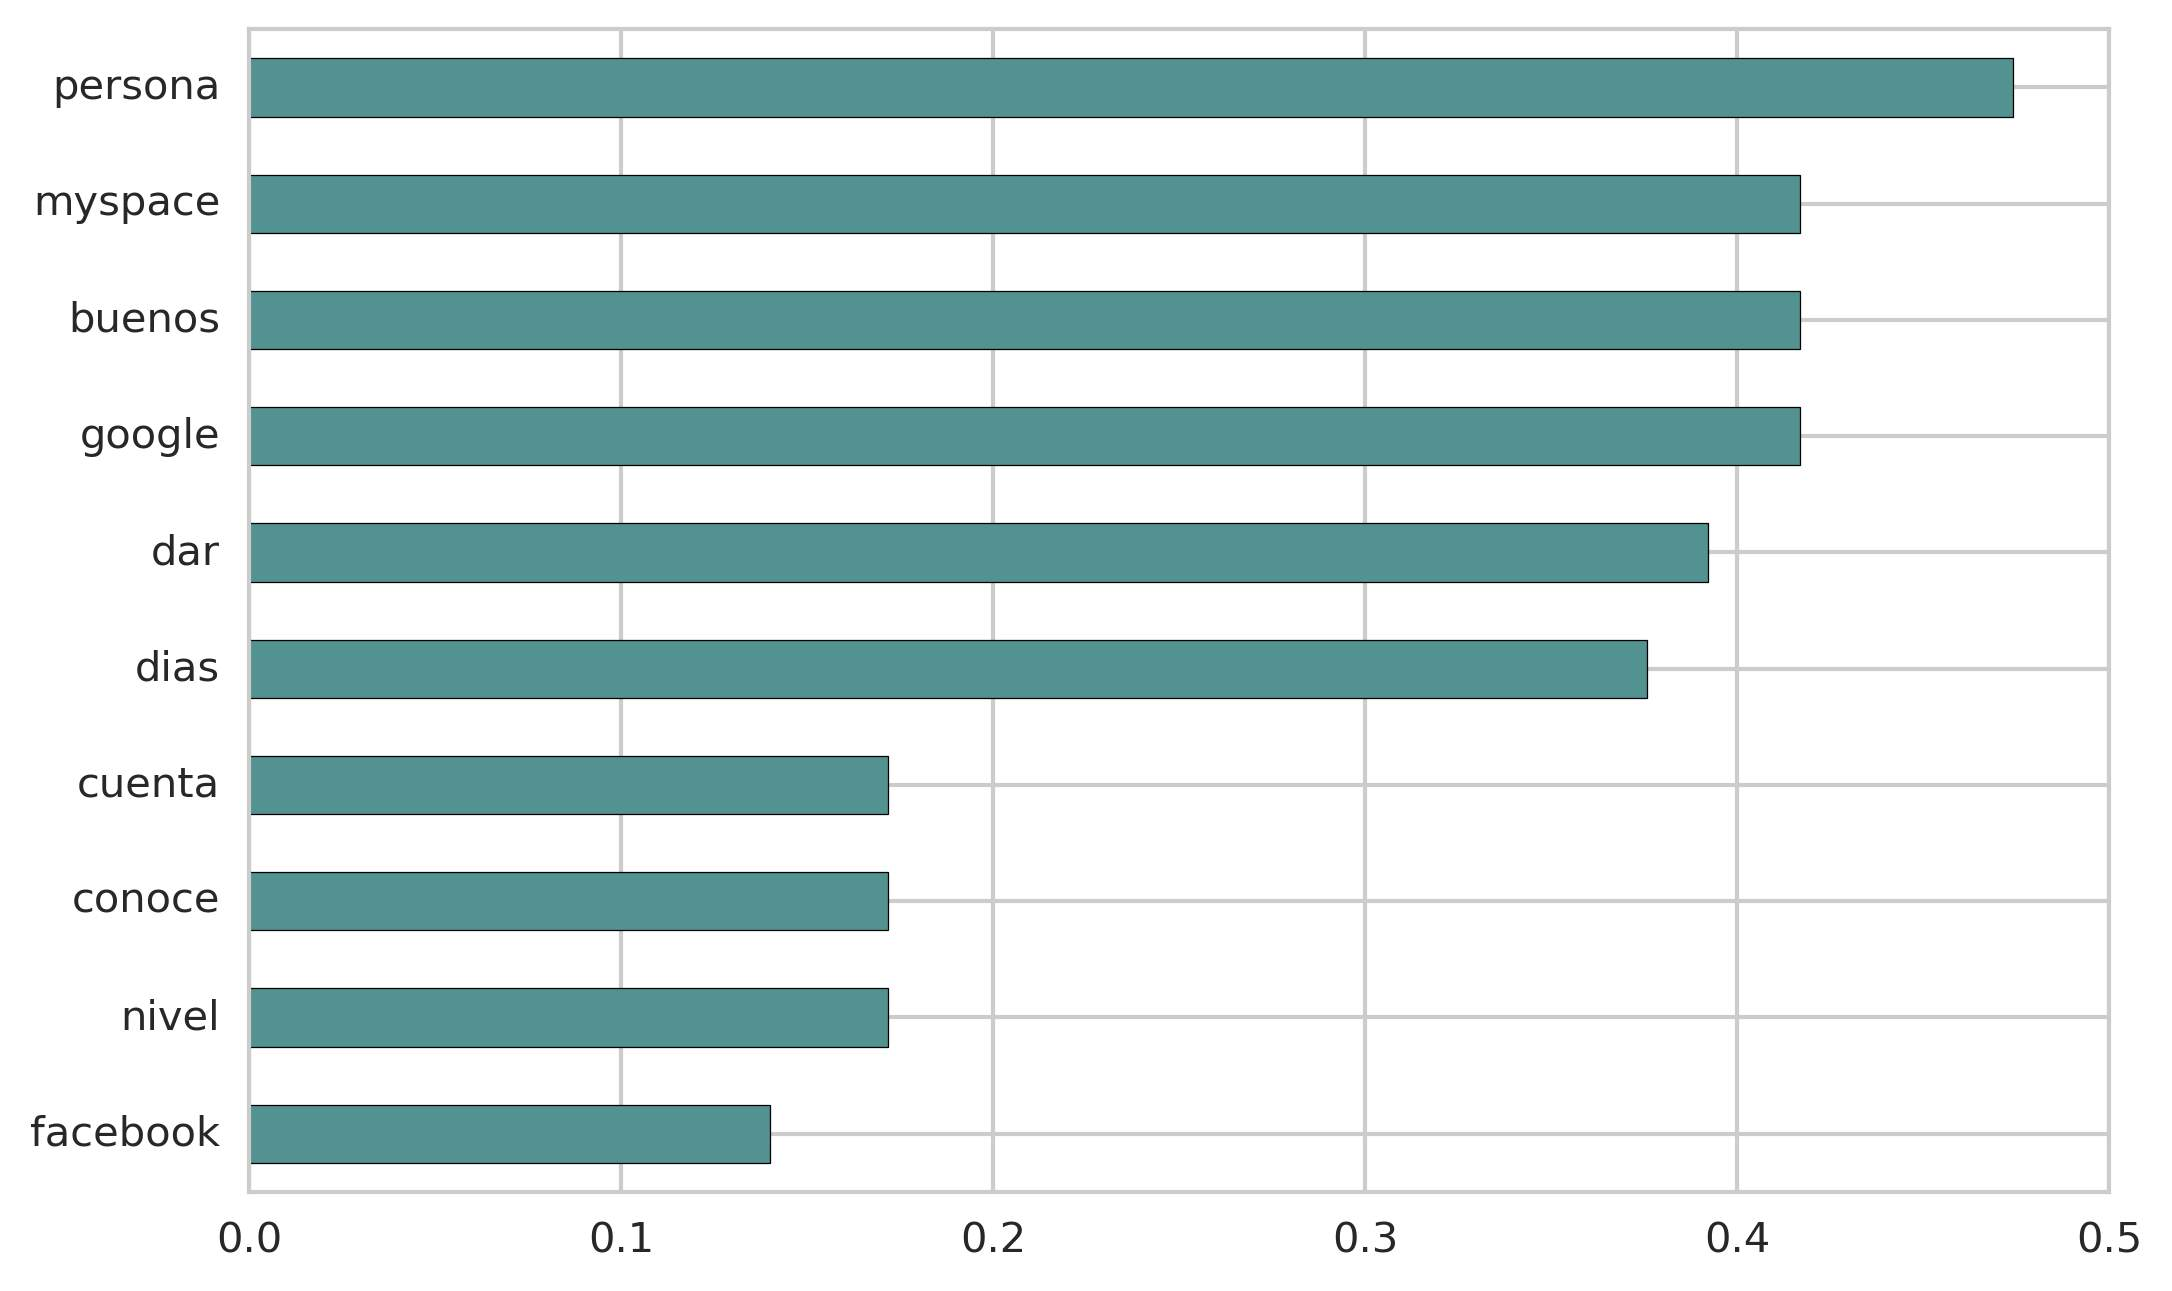
\includegraphics[width=\textwidth]{twitter_murcia/report_images/topic-06-terms.jpg}
    \end{subfigure}
\end{figure}

\begin{figure}[htbp!]
    \centering
    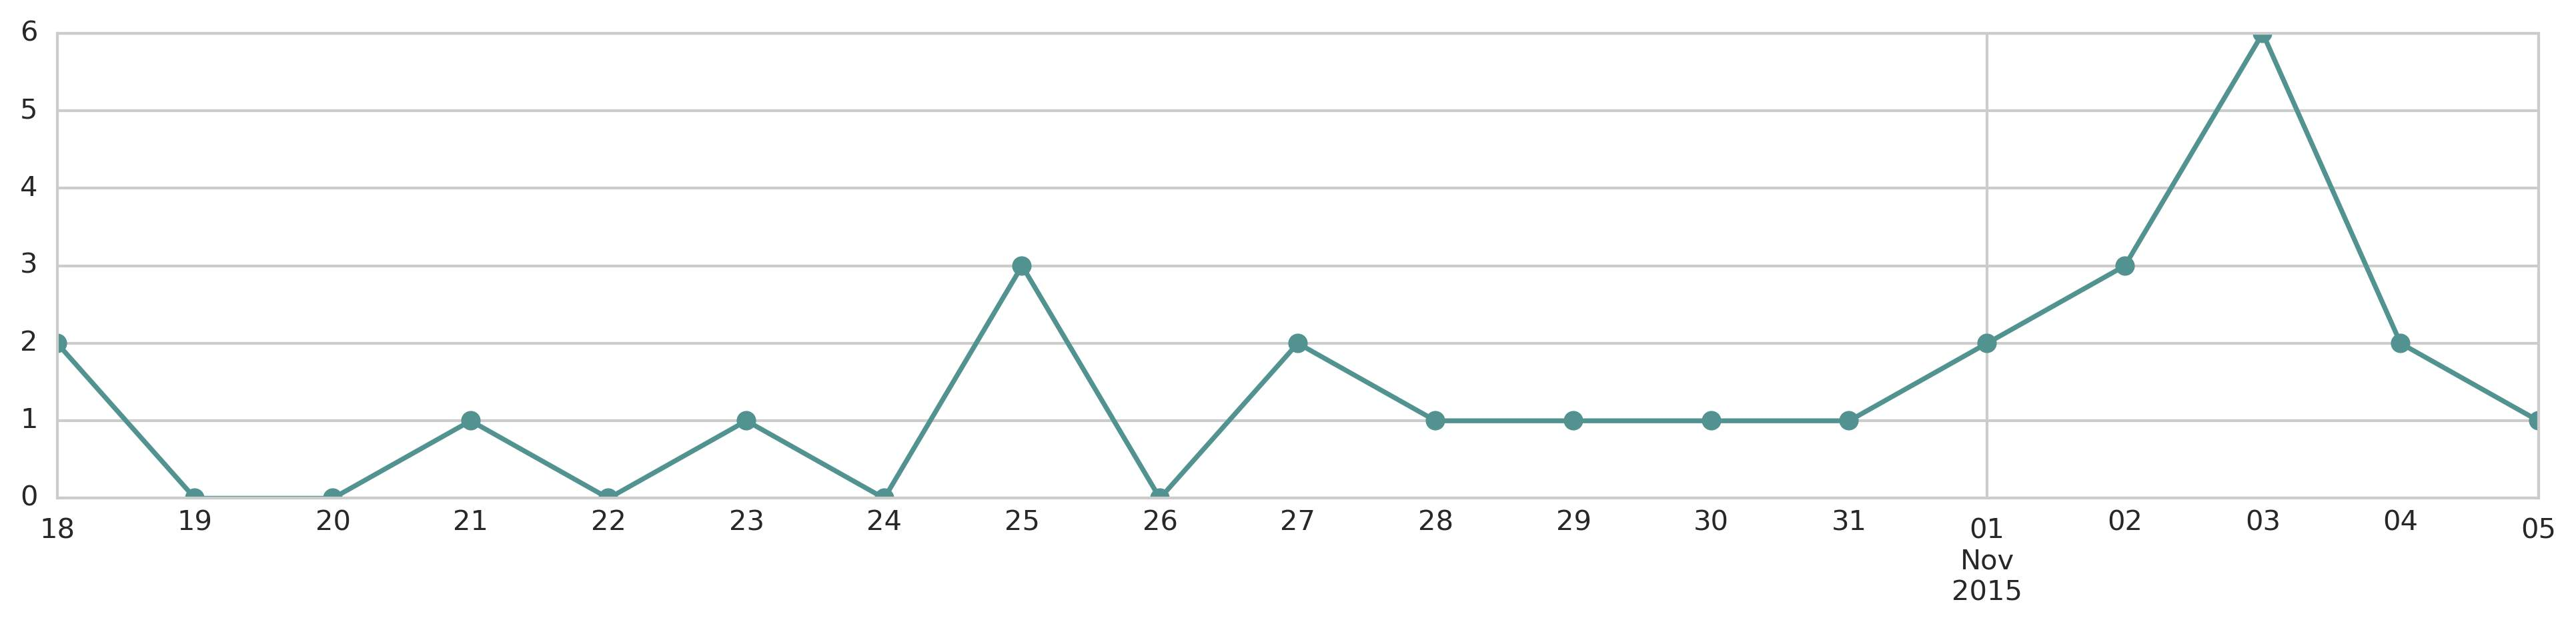
\includegraphics[width=\textwidth]{twitter_murcia/report_images/topic-06-timeseries.jpg}
\end{figure}

\rowcolors{2}{gray!25}{white}
\begin{longtable}{p{12.5cm}rr}
\toprule
Text & Count & Rel \\
\midrule
\endhead
\midrule
\multicolumn{3}{r}{{Continued on next page}} \\
\midrule
\endfoot

\bottomrule
\endlastfoot
@tuiteasotrabajs @mortajuza Bastante tiene con dar los buenos días en persona en Facebook, Twitter, Tuenti, Myspace, Google+, e-Darling... & 1 & 0.93 \\
\begin{tabular}[c]{@{}l@{}}Me estoy dando cuenta de que una persona no te conoce lo sufiente hasta que no le enseñas tu tuenti \\ Es un nuevo nivel en una relacion\end{tabular} & 1 & 0.43 \\
Todos tenemos pasados oscuros, como cuando poníamos en los estados de Tuenti los días que llevábamos con alguien. Y los tQ. Que no faltasen. & 1 & 0.34 \\
Meterse a tuenti y más formas de dar lache & 1 & 0.26 \\
RT @EvaTiritii: Llevo metiendome en tuenti 2 días y viendo fotos de mi novio. & 1 & 0.24 \\
RT @angelaruuiiz: Llevo leyenndo las mismas tonterias desde q me hice tuenti en 5° de primaria,a ver si renovamosss & 1 & 0.05 \\
RT @DaniJotaPe: Cuando utilizábamos el Tuenti y era así, molaba. http://t.co/Mp8OKGzk8t & 19 & 0.00 \\
RT @Ysucrist: como molaba Tuenti http://t.co/npzwIY8Zrk & 1 & 0.00 \\
@auronplay Agregame al tuenti ❤⭐ & 1 & 0.00 \\

\end{longtable}
\clearpage

\section{Topic 07}

\begin{figure}[htbp!]
    \centering
    \begin{subfigure}[b]{0.49\textwidth}
        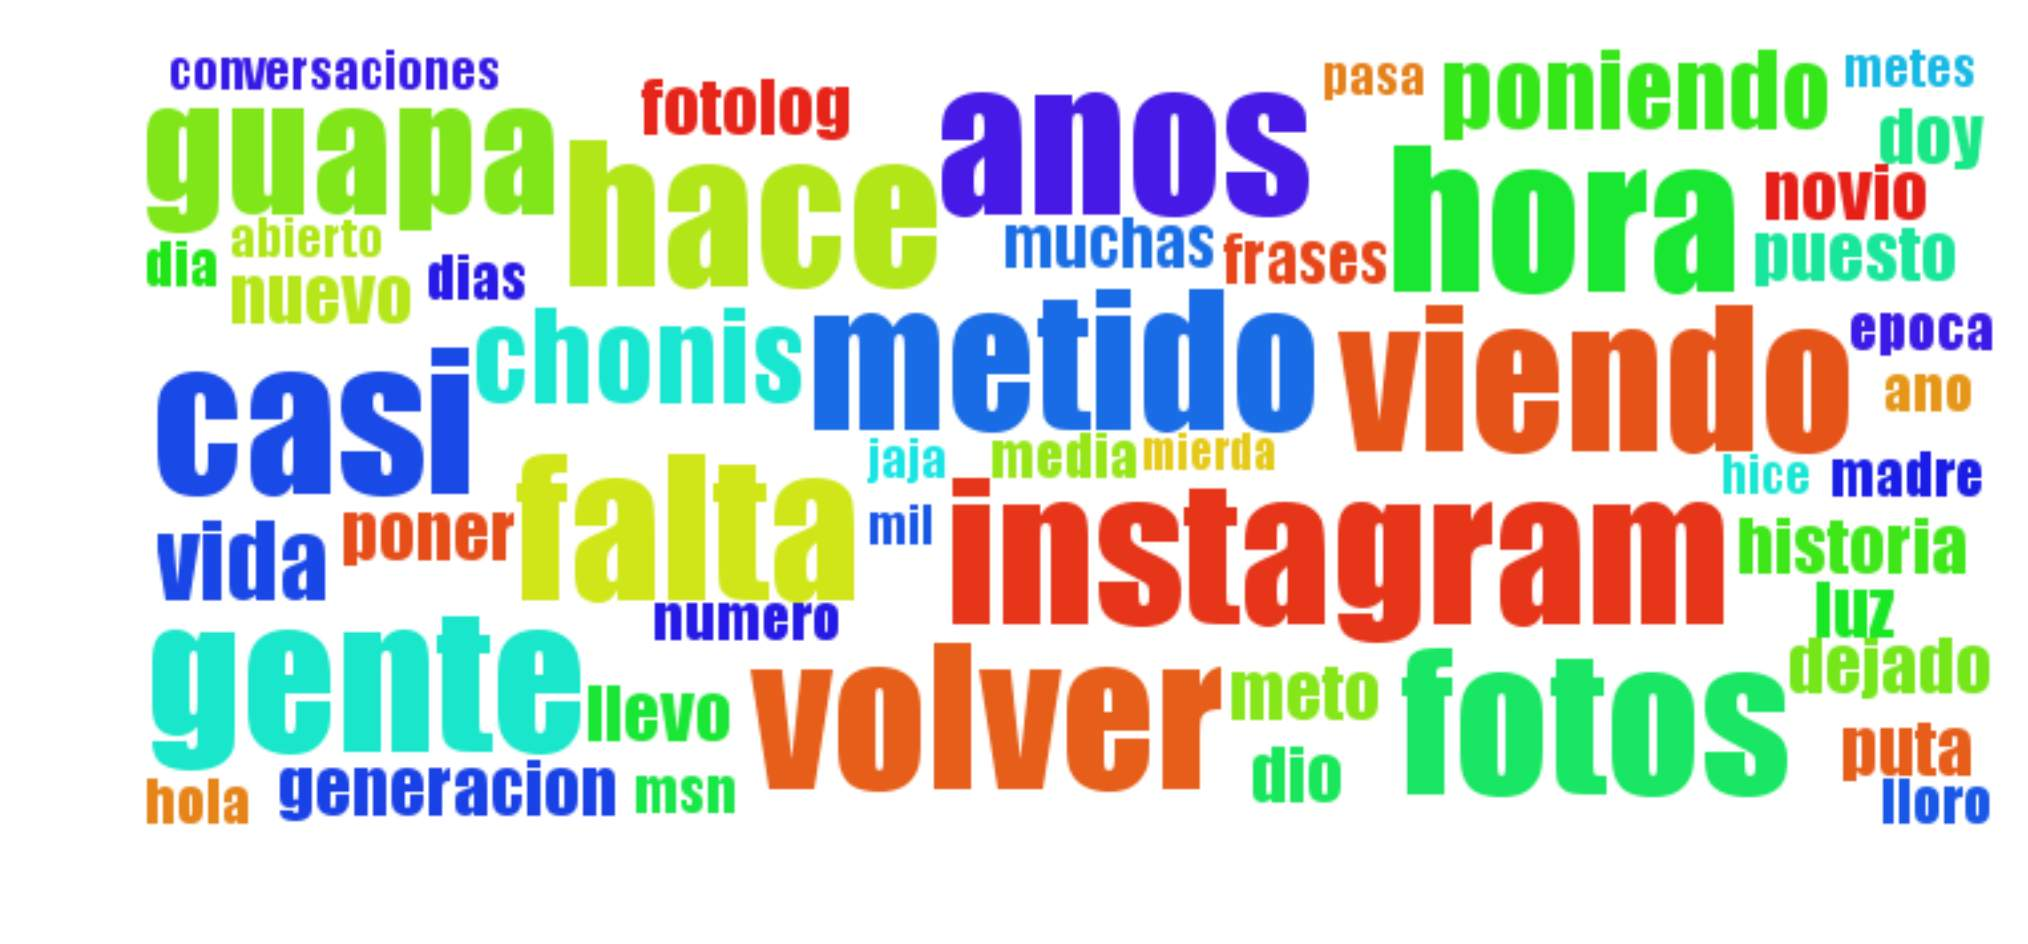
\includegraphics[width=\textwidth]{twitter_murcia/report_images/topic-07-wordcloud.jpg}
    \end{subfigure}
    \begin{subfigure}[b]{0.49\textwidth}
        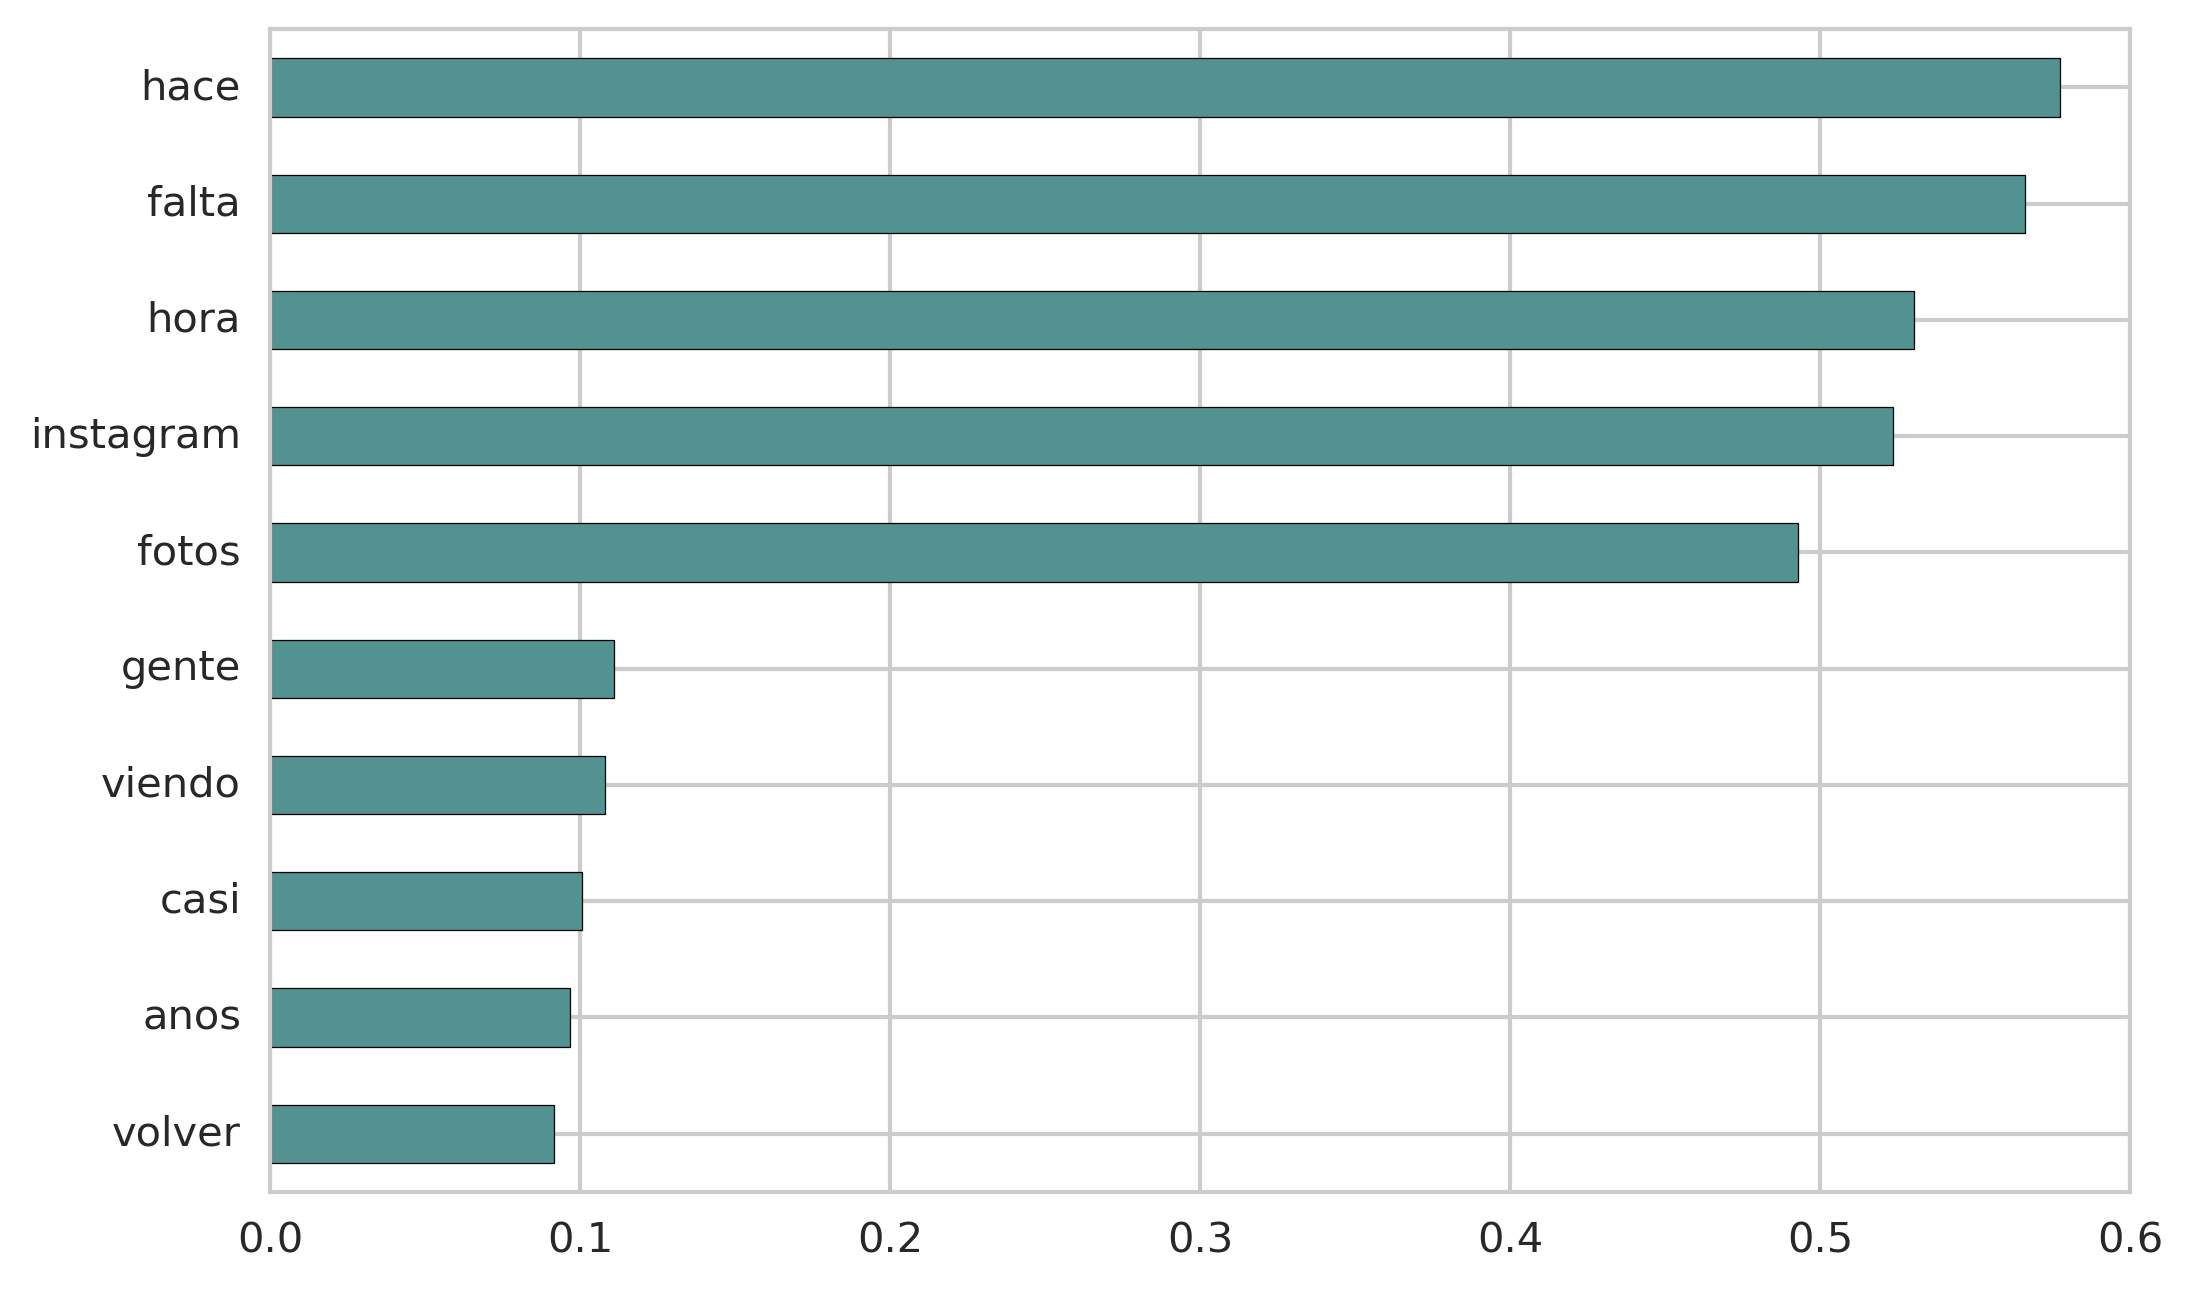
\includegraphics[width=\textwidth]{twitter_murcia/report_images/topic-07-terms.jpg}
    \end{subfigure}
\end{figure}

\begin{figure}[htbp!]
    \centering
    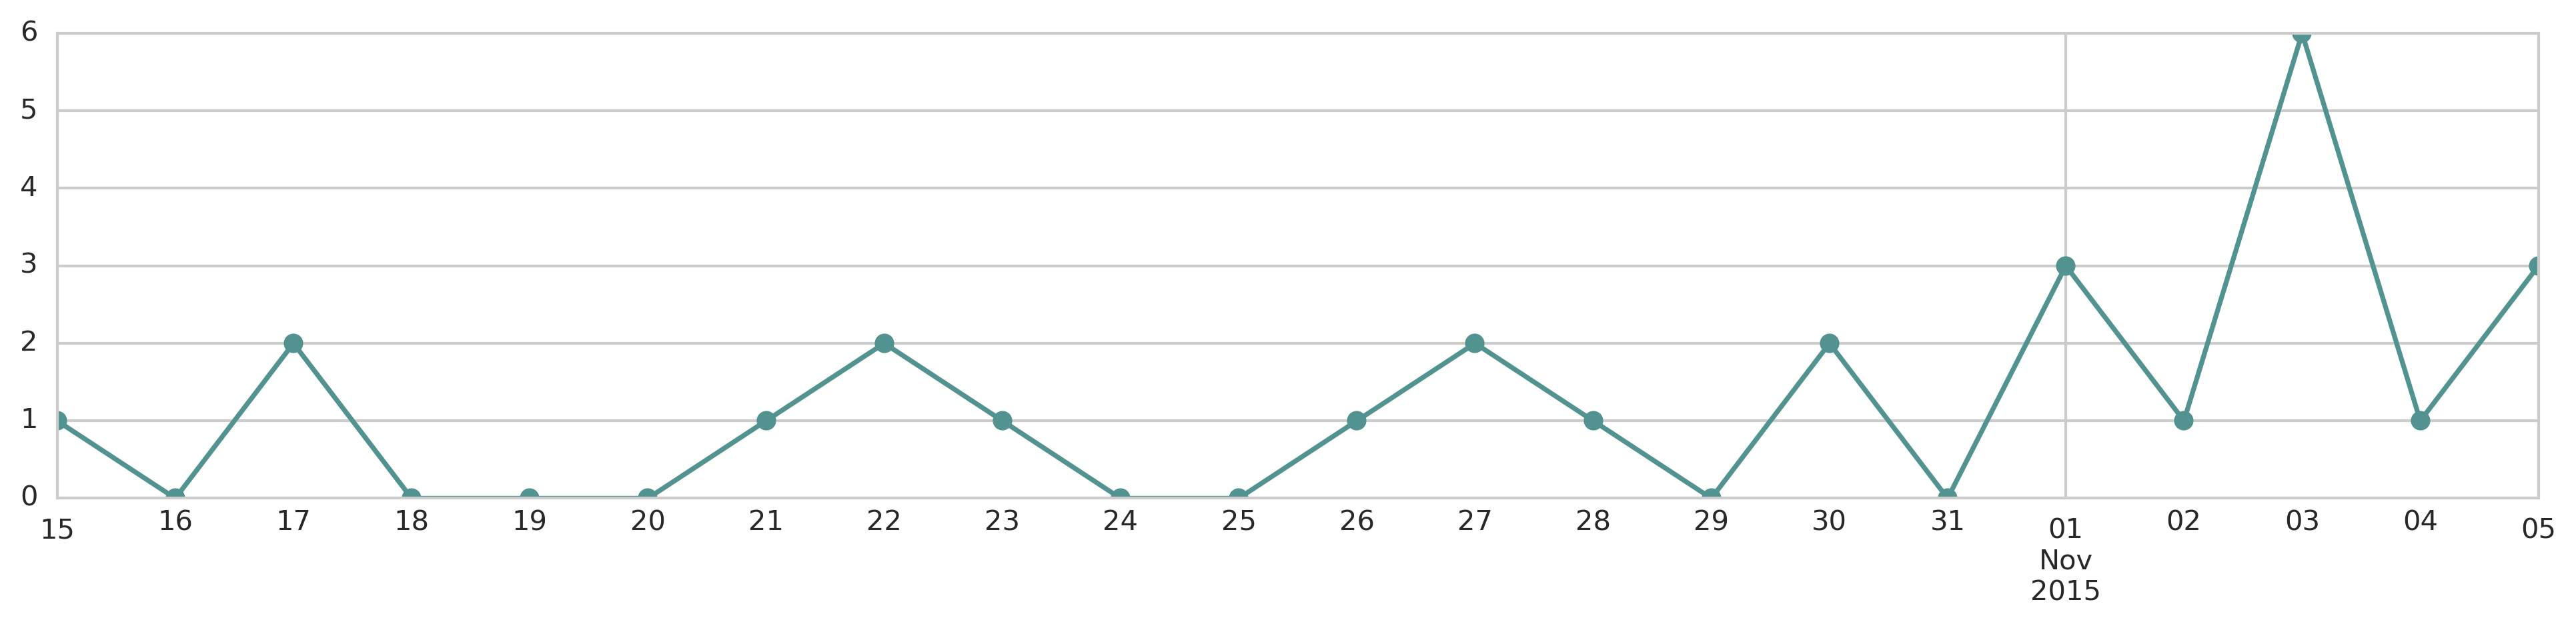
\includegraphics[width=\textwidth]{twitter_murcia/report_images/topic-07-timeseries.jpg}
\end{figure}

\rowcolors{2}{gray!25}{white}
\begin{longtable}{p{12.5cm}rr}
\toprule
Text & Count & Rel \\
\midrule
\endhead
\midrule
\multicolumn{3}{r}{{Continued on next page}} \\
\midrule
\endfoot

\bottomrule
\endlastfoot
RT @UnWhatsappEs: Algunos se creen que Instagram, es como Tuenti. A ver si os enteráis de que no hace falta que subáis 10 fotos a la hora. & 6 & 0.95 \\
@Jannyfer25 instagram no es tuenti & 1 & 0.42 \\
RT @LoLViictor: @Jannyfer25 instagram no es tuenti & 1 & 0.42 \\
RT @pablomosto: Hay gente que confunde Instagram con Tuenti y sube 20 fotos del tirón. & 2 & 0.34 \\
RT @RickyNumberFive: Hora de volver al tuenti. & 1 & 0.30 \\
RT @Daniru\_\_: Es la hora de volver a Tuenti. & 2 & 0.30 \\
Antes me he metido a tuenti y casi me da un algo viendo como escribía y lo guapa que era hace tres años.😨 & 1 & 0.27 \\
@loveinbooks\_ uii si viéramos las fotos del tuenti de más de uno/a (me incluyo) jajajajajjaa & 1 & 0.27 \\
Admitamoslo señores, el instagram es el nuevo tuenti. Le doy dos años mas de vida antes de que nos aburramos de el. & 1 & 0.18 \\
RT @TuiterHits: Chonis que suben fotos al Tuenti poniendo: "Etiketarse kien kiera". ¡PERO QUIEN SE VA A ETIQUETAR EN ESO, DESGRACIADA! & 2 & 0.16 \\
Un poco de historia: Los poetas babosos de Instagram son la 3ª generación de la poesia amorosa, todo comenzo en fotolog y siguio en tuenti. & 1 & 0.14 \\
RT @DanielG\_Lopez: Sólo me meto a Instagram cuando estoy cagando, imaginaros lo que me importan vuestras selfies con frases del Tuenti. & 1 & 0.13 \\
"En \#tuenti tenemos muchas fotos de nuestra vida que hemos dejado olvidadas", @JMMartiGuti \#TertuliaUniversitaria http://t.co/a7PlxPTq4F & 1 & 0.12 \\
Recordáis cuando nuestro éxito se media por el número de mg que tenían nuestras fotos de tuenti tomadas en el espejo  o con la webcam? & 1 & 0.11 \\
Me he metido en tuenti y JAJAJAJAJAJJA & 1 & 0.07 \\
Hola, guapa, ¿Tienes Tuenti? & 1 & 0.06 \\
RT @Desvirgaviejas: Hola, guapa, ¿Tienes Tuenti? & 1 & 0.06 \\
Ver tuenti y querer volver al año 2009 😢😢 & 1 & 0.04 \\
Es tan Tuenti 2010. https://t.co/RFBhveqER4 & 1 & 0.00 \\

\end{longtable}
\clearpage

\section{Topic 08}

\begin{figure}[htbp!]
    \centering
    \begin{subfigure}[b]{0.49\textwidth}
        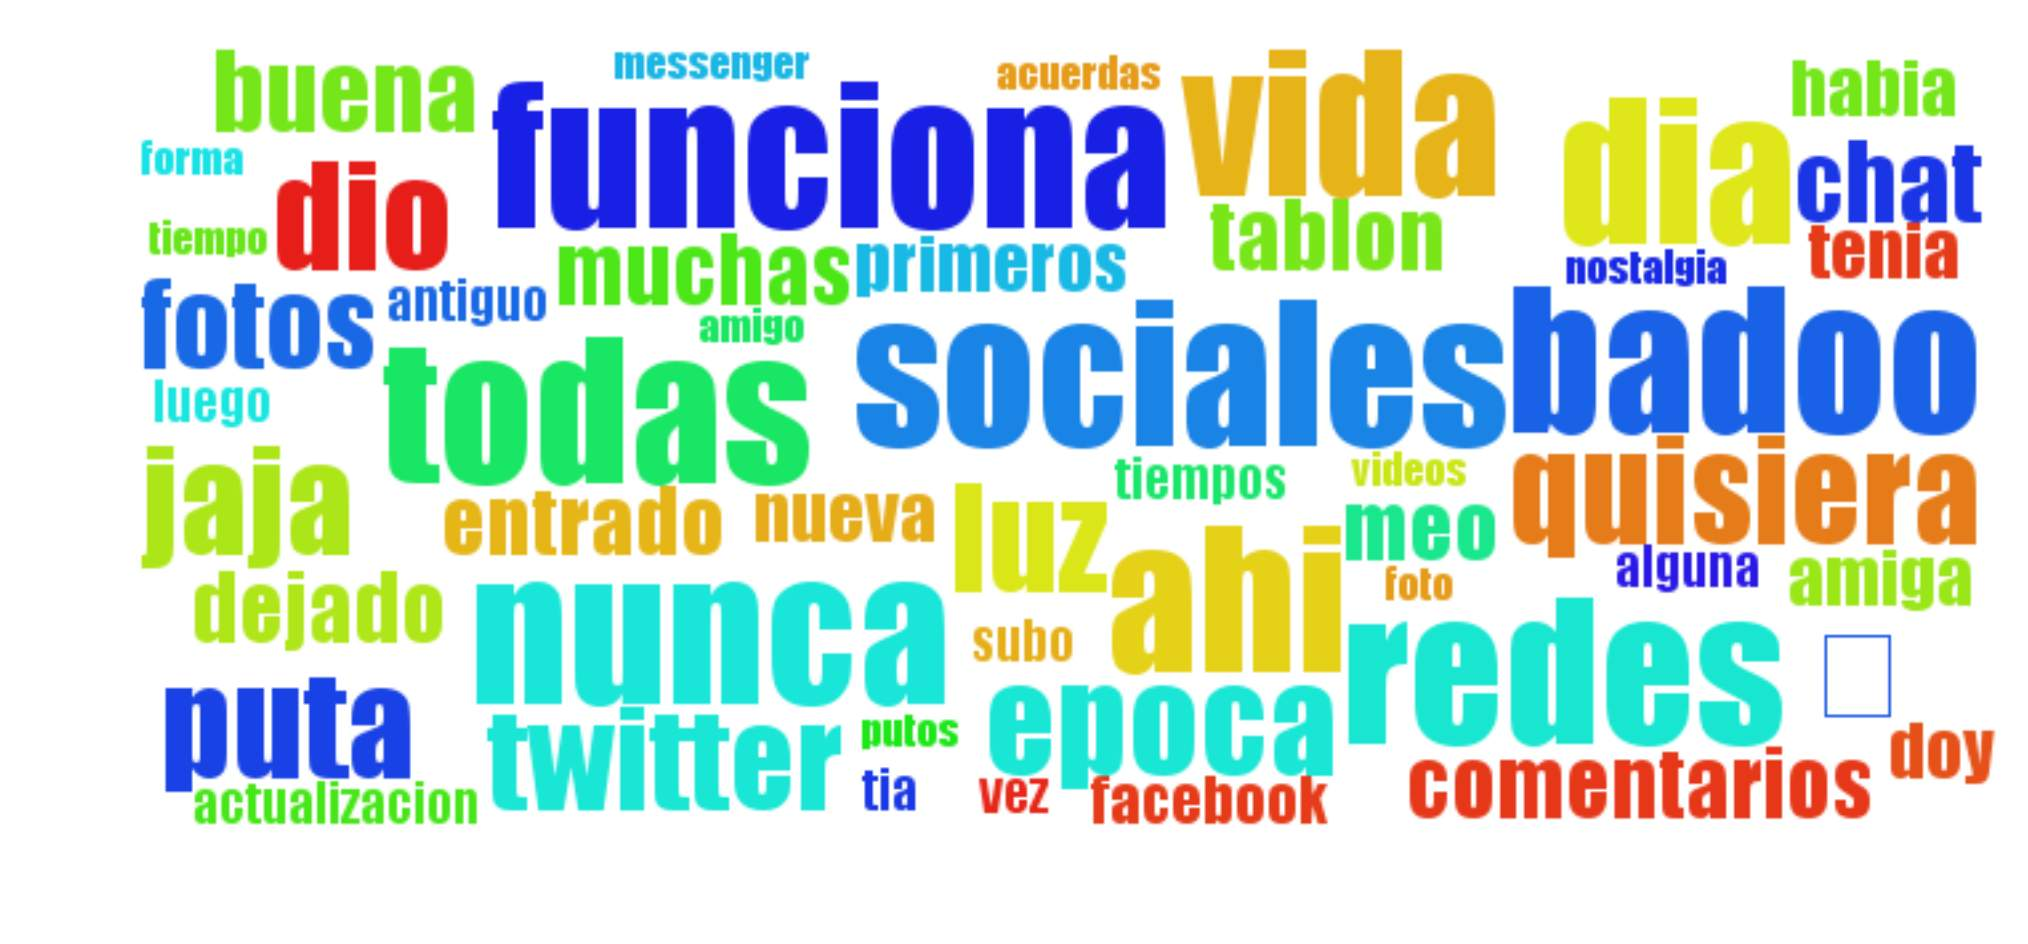
\includegraphics[width=\textwidth]{twitter_murcia/report_images/topic-08-wordcloud.jpg}
    \end{subfigure}
    \begin{subfigure}[b]{0.49\textwidth}
        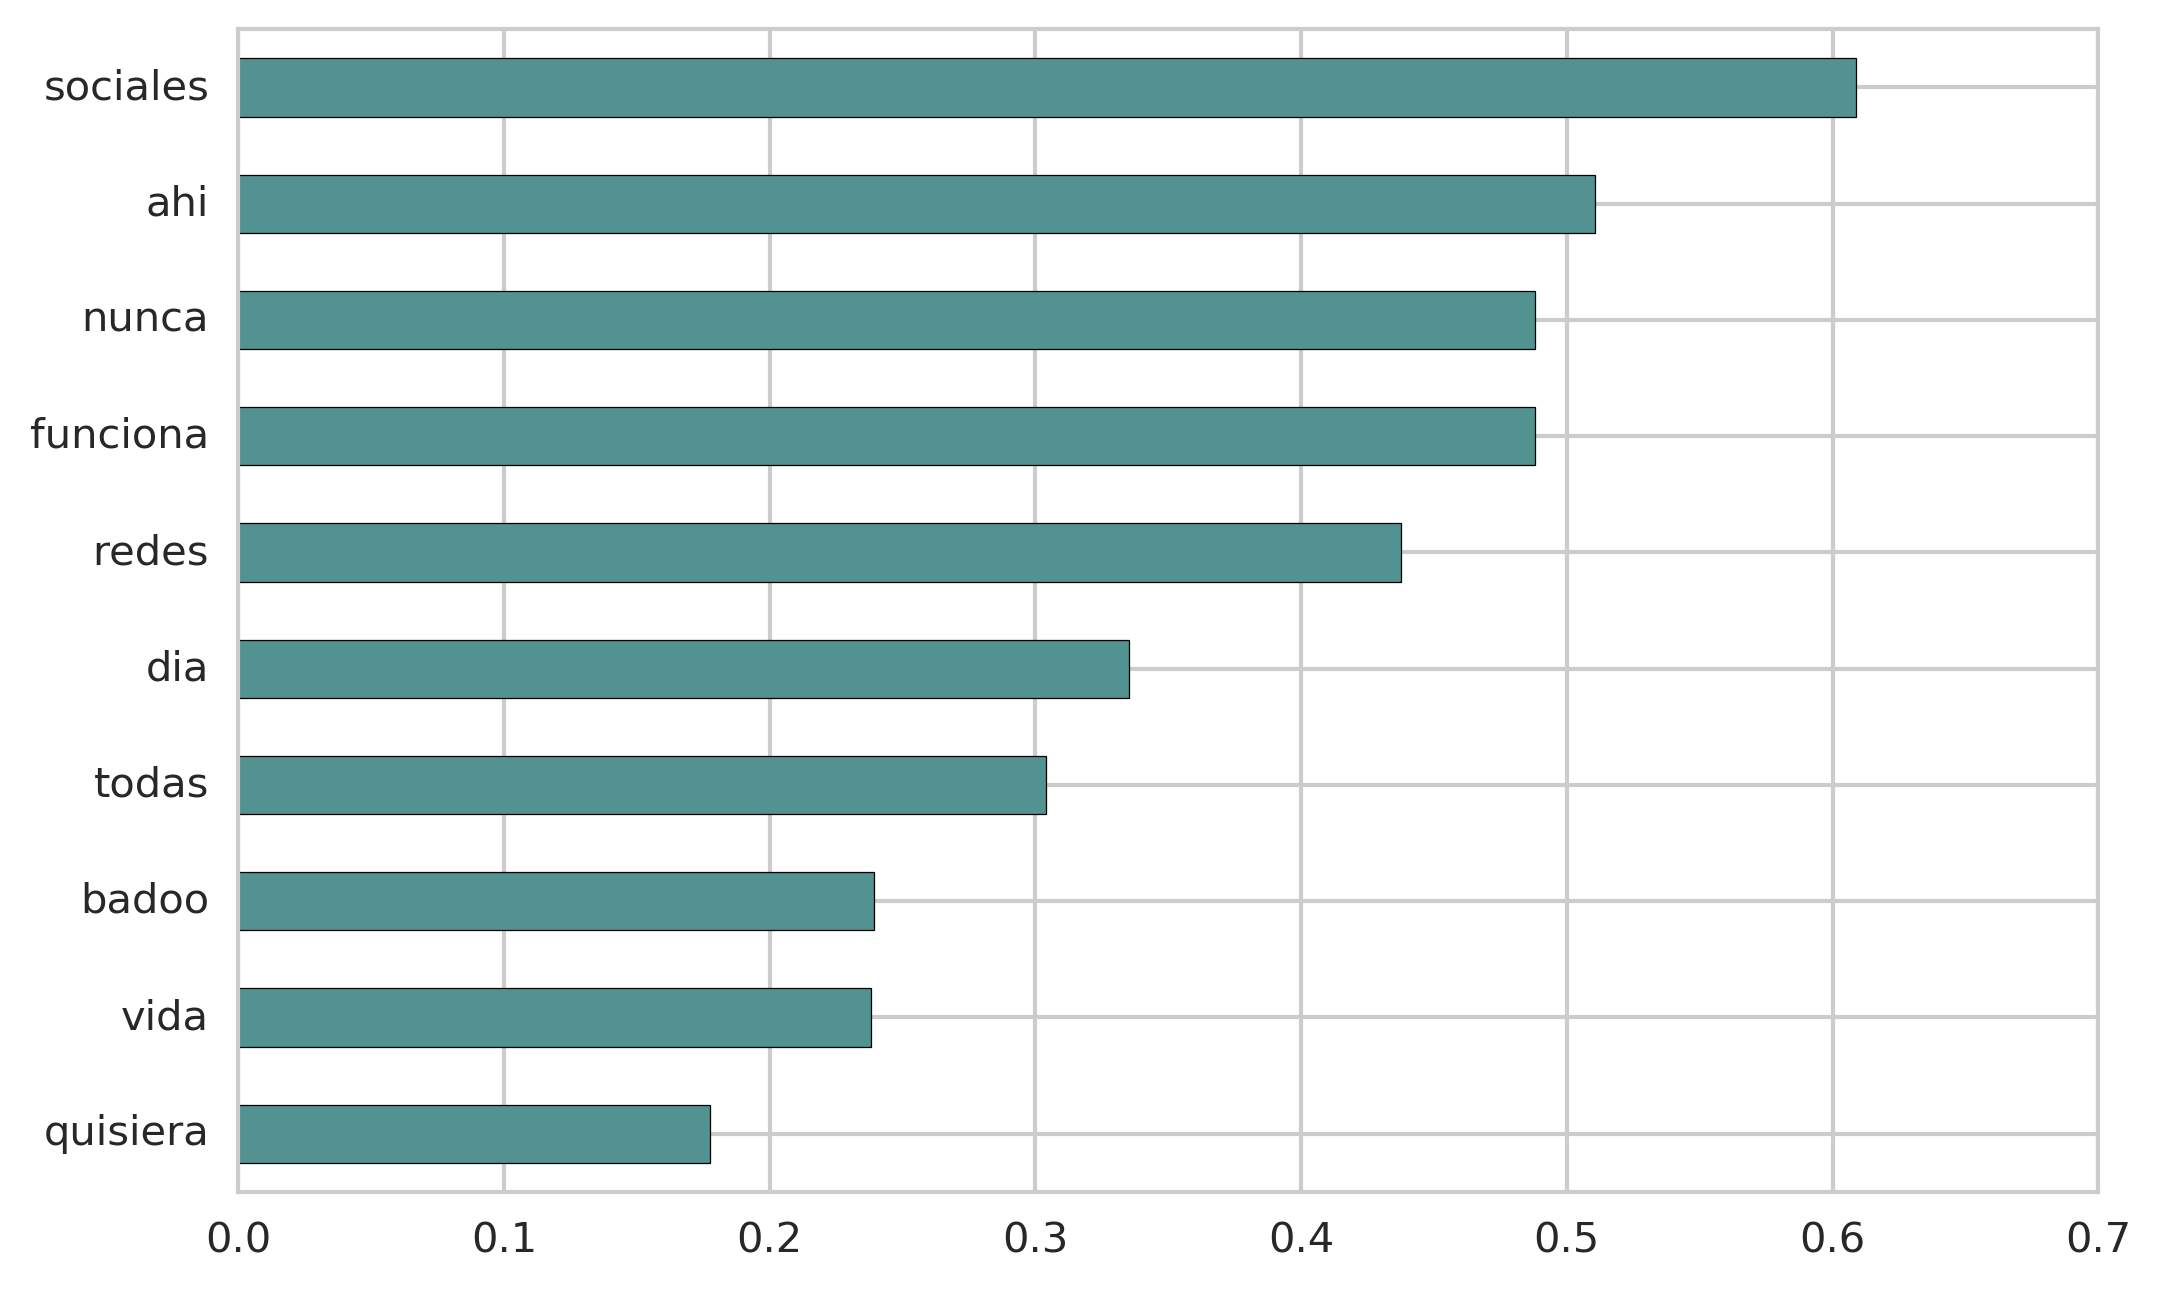
\includegraphics[width=\textwidth]{twitter_murcia/report_images/topic-08-terms.jpg}
    \end{subfigure}
\end{figure}

\begin{figure}[htbp!]
    \centering
    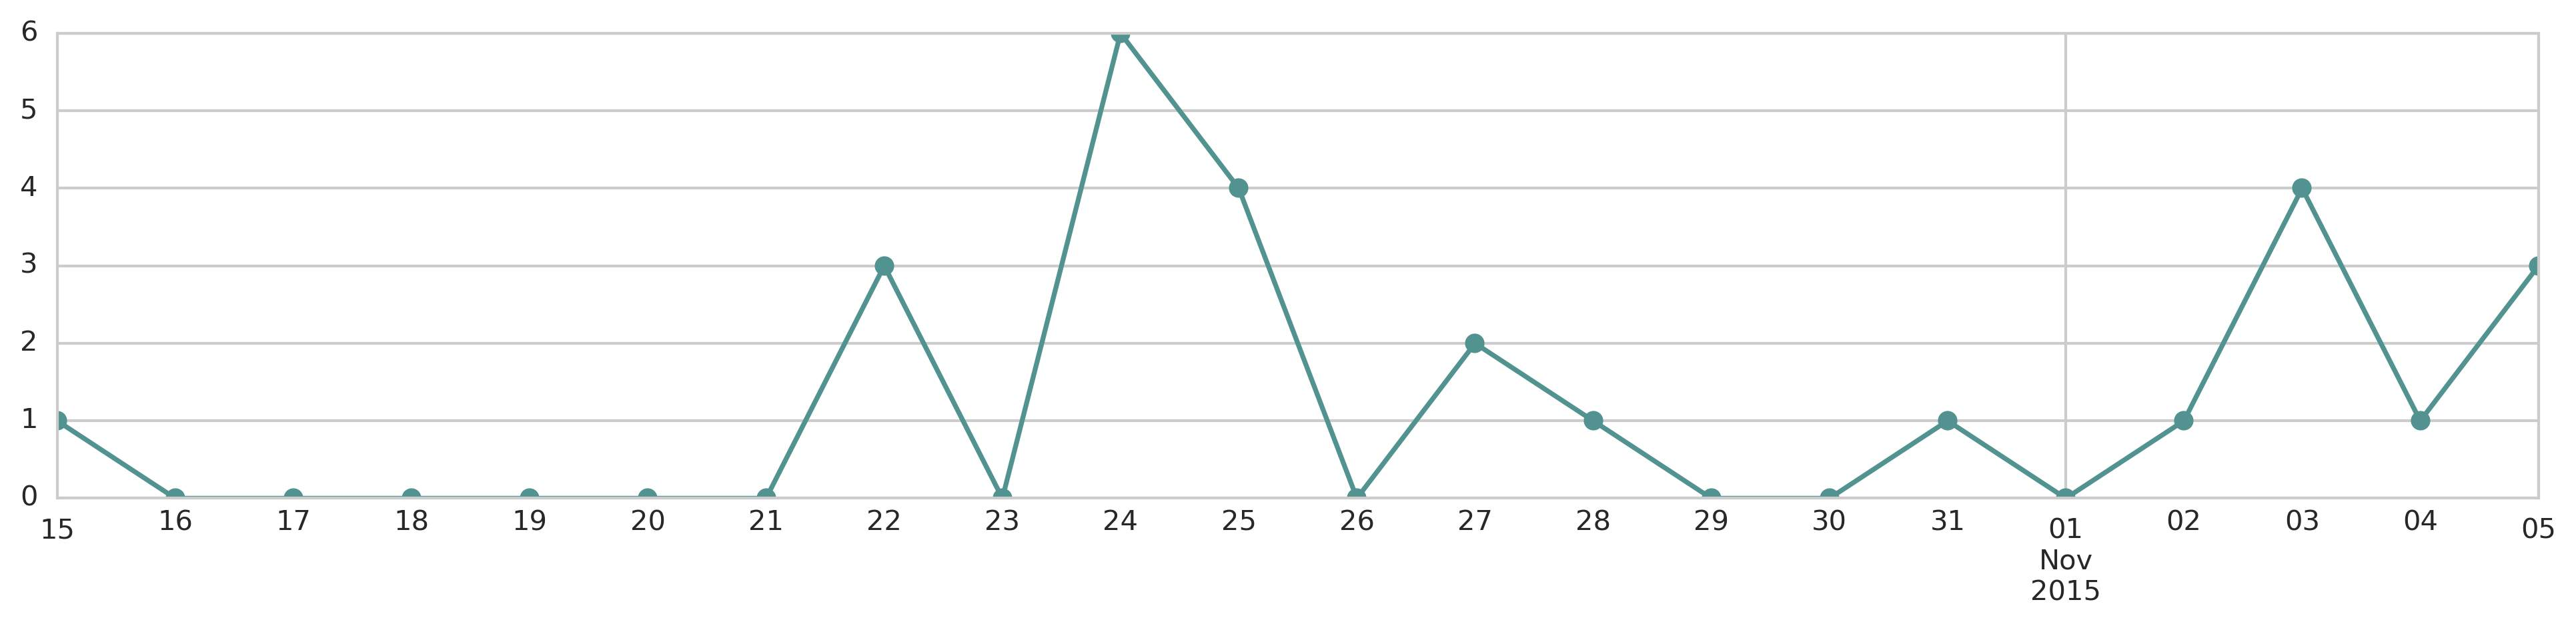
\includegraphics[width=\textwidth]{twitter_murcia/report_images/topic-08-timeseries.jpg}
\end{figure}

\rowcolors{2}{gray!25}{white}
\begin{longtable}{p{12.5cm}rr}
\toprule
Text & Count & Rel \\
\midrule
\endhead
\midrule
\multicolumn{3}{r}{{Continued on next page}} \\
\midrule
\endfoot

\bottomrule
\endlastfoot
RT @FranciscodPaula: Nunca entenderé los continuos cambios en las Redes Sociales. Si funciona, para que lo tocas! Ahí tenemos el ejemplo de… & 2 & 0.82 \\
\begin{tabular}[c]{@{}l@{}}Que Perea abandona twitter el día 31!! Y todas las Redes Sociales. El tuenti, el badoo... \\  \\ Sus asesores mandan. \\  \\  https://t.co/foPSYAqMqS\end{tabular} & 1 & 0.56 \\
¿Por qué todas las redes sociales como tuenti y ahora Twitter acaban copiando a Facebook? & 1 & 0.52 \\
@IreneMartinez98 JAJAJAJAJAJA si quisiera joderte la vida buscaría en tuenti ahí sí que hay material 😂😂 & 1 & 0.38 \\
RT @Siegg\_erreape: @IreneMartinez98 JAJAJAJAJAJA si quisiera joderte la vida buscaría en tuenti ahí sí que hay material 😂😂 & 1 & 0.38 \\
@levsad la época tuenti nos dio la puta vida, posdata tengo fotos comprometedoras tuyas, un día saldrán a la luz & 1 & 0.35 \\
RT @merybarcelo124: @jdom\_patri y yo recordando lo infumable que fue nuestra época Tuenti. & 1 & 0.11 \\
@TisioMolina eso es de la época tuenti JAJAJAJAJAJAJAJAJAJ que buena & 1 & 0.10 \\
RT @levsad: @TisioMolina eso es de la época tuenti JAJAJAJAJAJAJAJAJAJ que buena & 1 & 0.10 \\
Esa época en la que se usaban los comentarios de Tuenti como chat. & 1 & 0.07 \\
RT @Canovastelee: Esa época en la que se usaban los comentarios de Tuenti como chat. & 1 & 0.07 \\
\begin{tabular}[c]{@{}l@{}}Yo tenía una amiga de Galicia en la época tuenti.  \\  \\ Más que las gallinas era\end{tabular} & 1 & 0.05 \\
\begin{tabular}[c]{@{}l@{}}De mis primeros vídeos que colgué en el tablón de Tuenti, allá por 2000 y algo, en mi época gayer más colorida. \\  \\ https://t.co/wwZtbivoVd\end{tabular} & 1 & 0.05 \\
\begin{tabular}[c]{@{}l@{}}RT @Sickfilis: En mis tiempos se ligaba de otra forma. \\ Por messenger. Y luego le dejabas indirectas en el tablón de tuenti. \\ Eso si era liga…\end{tabular} & 1 & 0.02 \\
Que nostalgia ver los comentarios del Tuenti :( & 1 & 0.01 \\
Hay personajes y luego esta @lucia95qp en sus tiempos de tuenti a topeeeeee!! & 1 & 0.01 \\
Yo también tenia un amigo que me comentaba en todos los putos estados de Tuenti que publicaba. Me los jodía todos. & 1 & 0.01 \\
Ola wapa das tuenti? 😜 @IreneMartinez98 & 1 & 0.00 \\
\begin{tabular}[c]{@{}l@{}}RT @myfabdirection: 😼 uno u otro 😼  \\ \#EMABieggestFans1D  \\ Vota y rt si quieres🤐 \\  \\ ¿tuviste tuenti?\end{tabular} & 6 & 0.00 \\
RT @android\_esp: ¿Eres cliente de .Tuenti? Ya tienes un descuento del 15\% en terminales bq https://t.co/6wrHa80qjq \#BQAquarisM5 \#Andro4all & 1 & 0.00 \\

\end{longtable}
\clearpage

\section{Topic 09}

\begin{figure}[htbp!]
    \centering
    \begin{subfigure}[b]{0.49\textwidth}
        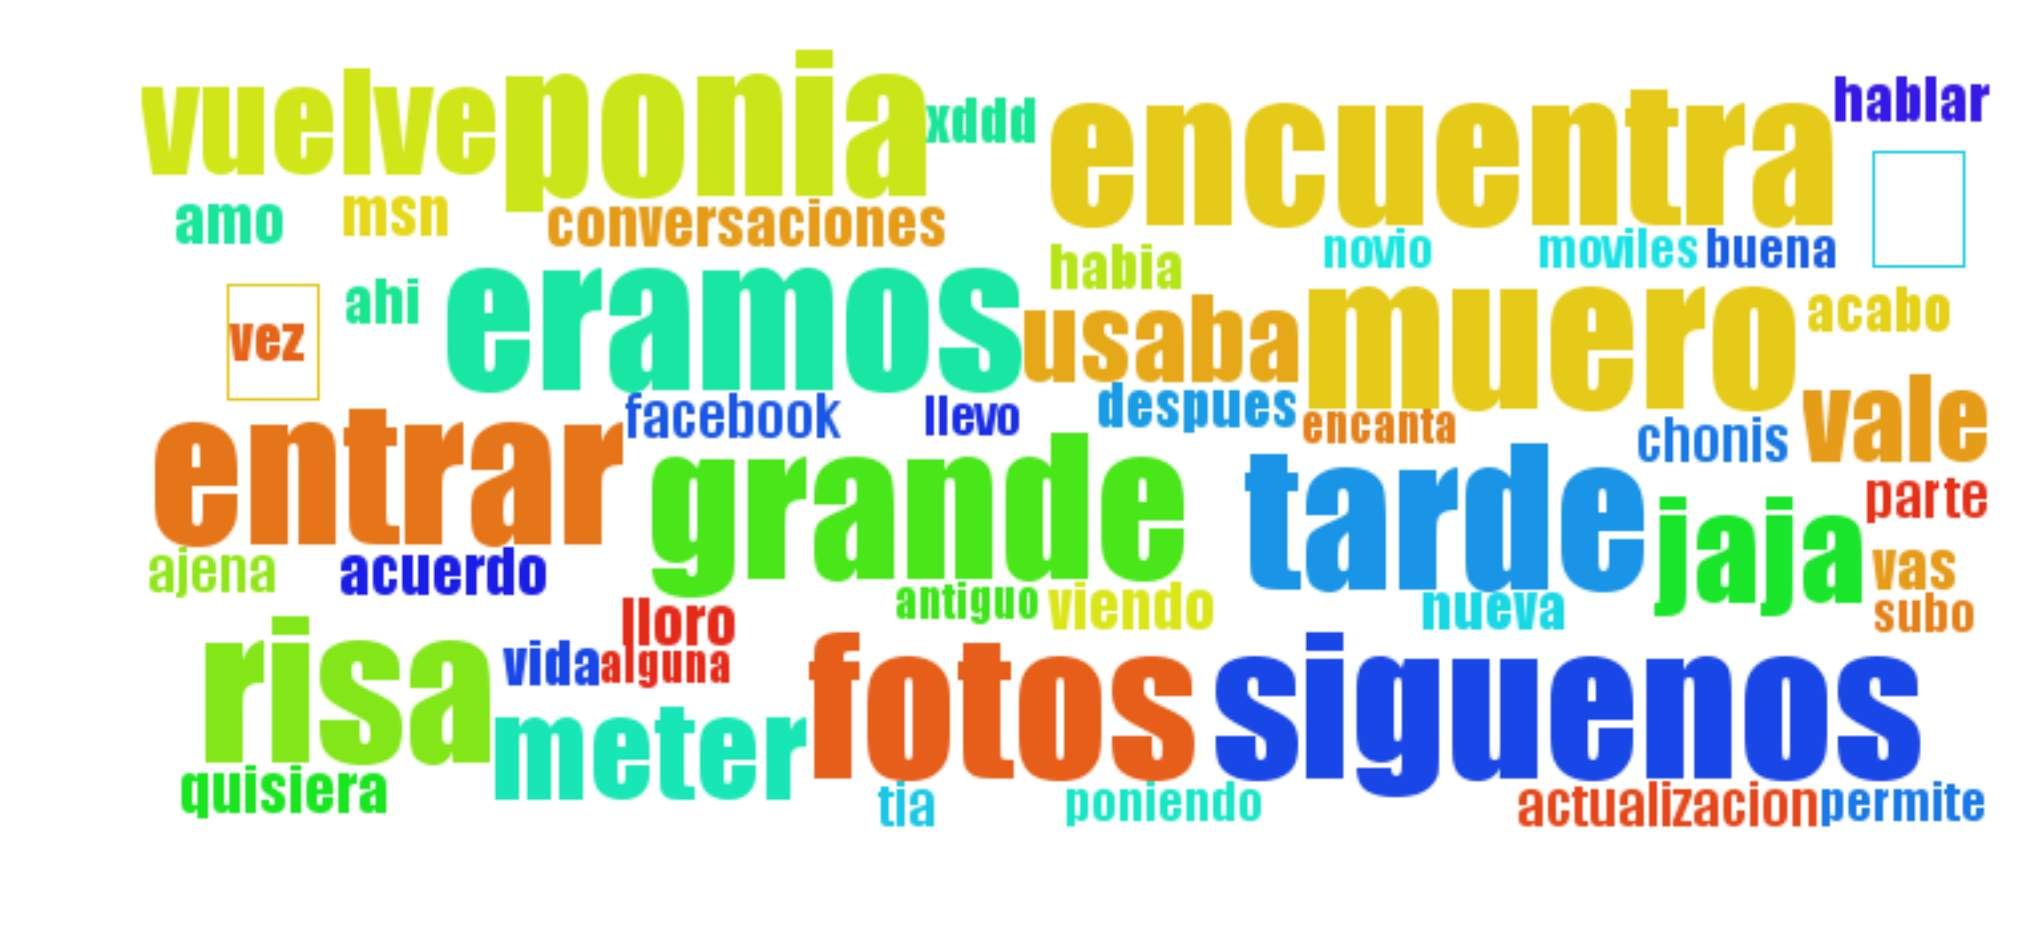
\includegraphics[width=\textwidth]{twitter_murcia/report_images/topic-09-wordcloud.jpg}
    \end{subfigure}
    \begin{subfigure}[b]{0.49\textwidth}
        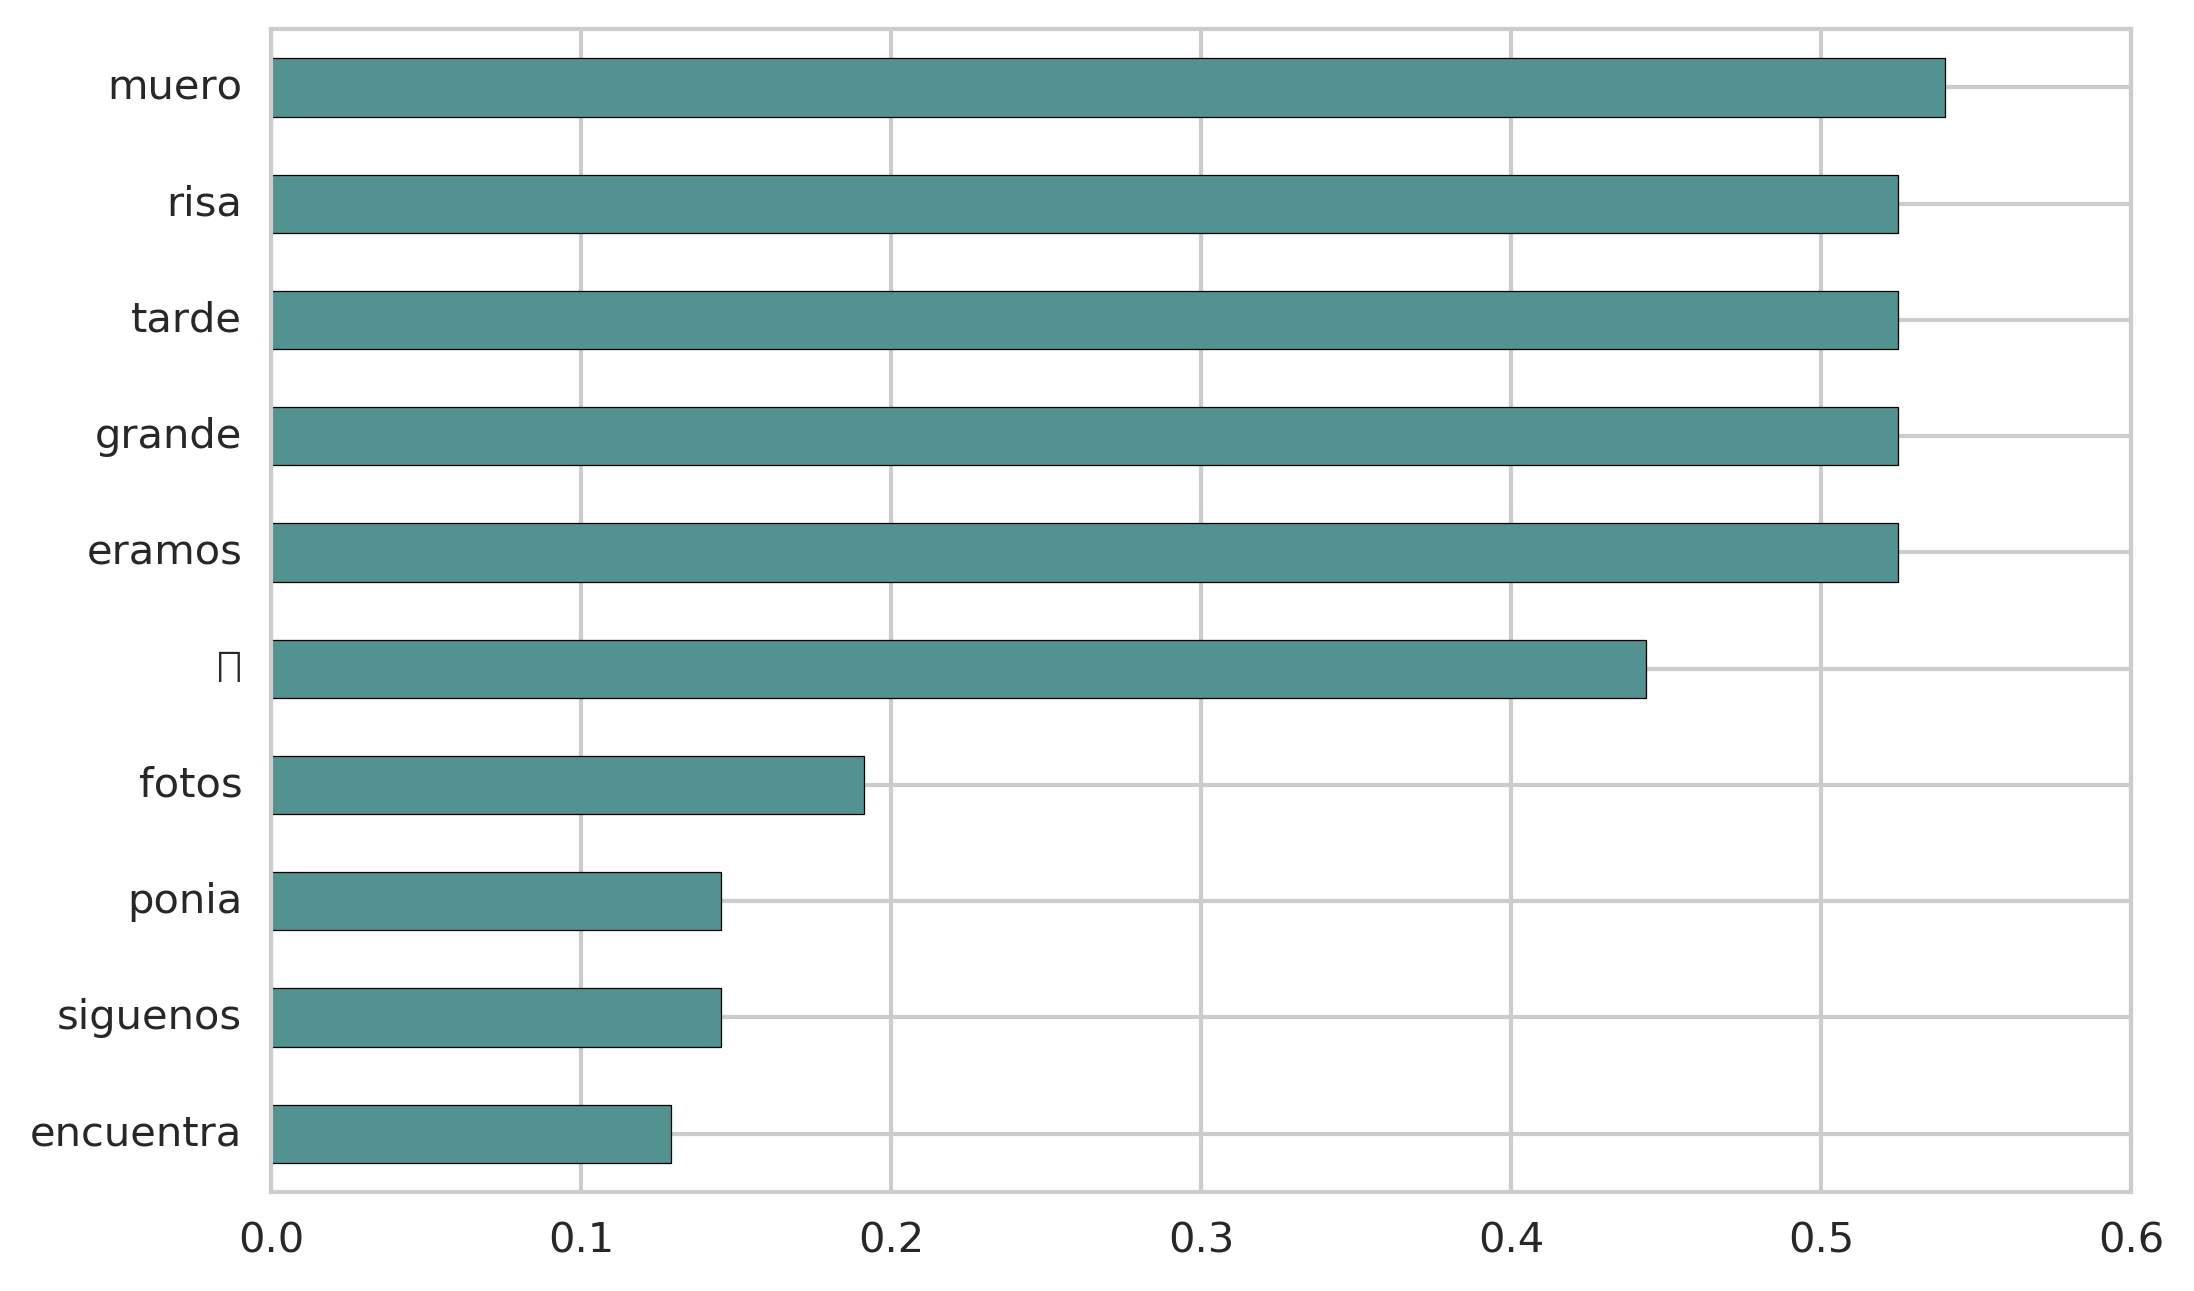
\includegraphics[width=\textwidth]{twitter_murcia/report_images/topic-09-terms.jpg}
    \end{subfigure}
\end{figure}

\begin{figure}[htbp!]
    \centering
    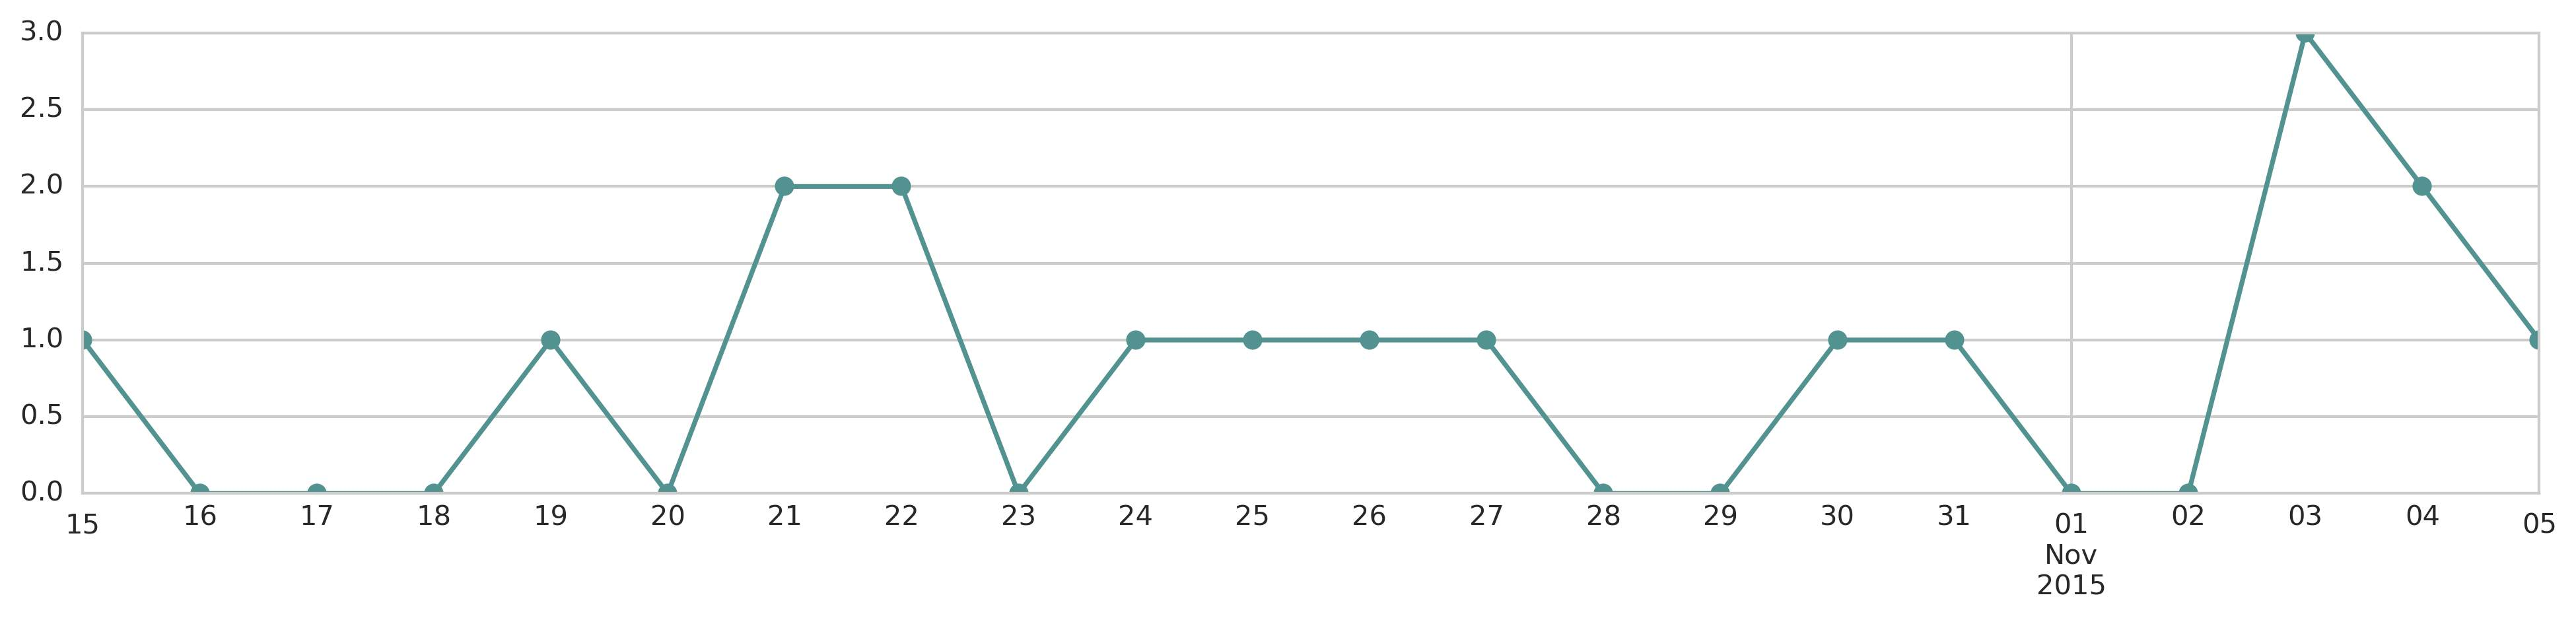
\includegraphics[width=\textwidth]{twitter_murcia/report_images/topic-09-timeseries.jpg}
\end{figure}

\rowcolors{2}{gray!25}{white}
\begin{longtable}{p{12.5cm}rr}
\toprule
Text & Count & Rel \\
\midrule
\endhead
\midrule
\multicolumn{3}{r}{{Continued on next page}} \\
\midrule
\endfoot

\bottomrule
\endlastfoot
Me muero de risa esta tarde con las fotos del tuenti 😂😂😂 Que grande eramos cohoneeee! 😂😂😂 & 1 & 0.90 \\
\begin{tabular}[c]{@{}l@{}}Acabo de ver una tienda y en el escaparate ponía: "siguenos en tuenti."  \\ Me muero JAJAJAJA\end{tabular} & 1 & 0.33 \\
Lo que se encuentra una cuando vuelve a entrar a Tuenti😭😂😂 & 1 & 0.23 \\
Lloro viendo tuenti 😂 lo que daría por ver conversaciones de "msn" & 1 & 0.17 \\
@AnaGon96 para mi son razones para vivir 😂😂😂😂 amo tuenti y te amo ti 💞 & 1 & 0.16 \\
RT @CarmenGomez14: @AnaGon96 para mi son razones para vivir 😂😂😂😂 amo tuenti y te amo ti 💞 & 1 & 0.16 \\
@DiOriginalNico hay que hablar con propiedad xDDD 😂😂 que esto ya no es tuenti & 1 & 0.11 \\
@CristinaPrez2 tuenti jajaja & 1 & 0.09 \\
RT @mariiazpt: @alitorralba\_ tia q en la nueva actualización en vez de estrellas hay corazones como en tuenti habia JAJAJAA & 1 & 0.06 \\
BQ y Tuenti lanzan juntos una promoción para dispositivos móviles: El acuerdo permite a  los clien... https://t.co/wnPFzXdybC \#publicidad & 1 & 0.05 \\
RT @javiitrejoo: AHORA TE METES A. TUENTI Y HAY 180 CONECTAOS JAJAJAJAJA PERSONAJES & 1 & 0.04 \\
Me encanta mirar el Tuenti de vez en cuando & 1 & 0.02 \\
RT @\_LuisCb97: Me encanta mirar el Tuenti de vez en cuando & 1 & 0.02 \\
Esto me recuerda a la actualizacion de tuenti que fue el declive absoluto de su existencia & 1 & 0.02 \\
@Salvajeman15 , mirar las de tuenti. & 1 & 0.01 \\
voy a meterme a mi tuenti a ver que me encuentro & 1 & 0.00 \\
Tuenti existe todavía? & 1 & 0.00 \\
RT @Nuuriaps: Lo q unió el tuenti q no lo separe nadie.👫 https://t.co/JjaqMTtKMD & 1 & 0.00 \\

\end{longtable}

